% This is the Reed College LaTeX thesis template. Most of the work
% for the document class was done by Sam Noble (SN), as well as this
% template. Later comments etc. by Ben Salzberg (BTS). Additional
% restructuring and APA support by Jess Youngberg (JY).
% Your comments and suggestions are more than welcome; please email
% them to cus@reed.edu
%
% See http://web.reed.edu/cis/help/latex.html for help. There are a
% great bunch of help pages there, with notes on
% getting started, bibtex, etc. Go there and read it if you're not
% already familiar with LaTeX.
%
% Any line that starts with a percent symbol is a comment.
% They won't show up in the document, and are useful for notes
% to yourself and explaining commands.
% Commenting also removes a line from the document;
% very handy for troubleshooting problems. -BTS

% As far as I know, this follows the requirements laid out in
% the 2002-2003 Senior Handbook. Ask a librarian to check the
% document before binding. -SN

%%
%% Preamble
%%
% \documentclass{<something>} must begin each LaTeX document
\documentclass[12pt,twoside]{reedthesis}
% Packages are extensions to the basic LaTeX functions. Whatever you
% want to typeset, there is probably a package out there for it.
% Chemistry (chemtex), screenplays, you name it.
% Check out CTAN to see: http://www.ctan.org/
%%

\usepackage[normalem]{ulem}
\usepackage[spanish,es-tabla]{babel}
\usepackage{setspace}\doublespacing
\usepackage{float}

\usepackage{graphicx,latexsym}
\usepackage{amsmath}
\usepackage{amssymb,amsthm}
\usepackage{longtable,booktabs,setspace}
\usepackage{chemarr} %% Useful for one reaction arrow, useless if you're not a chem major
\usepackage[hyphens]{url}
% Added by CII
\usepackage{hyperref}
\usepackage{lmodern}
\usepackage{float}
\floatplacement{figure}{H}
% End of CII addition
\usepackage{rotating}

% Next line commented out by CII
%%% \usepackage{natbib}
% Comment out the natbib line above and uncomment the following two lines to use the new
% biblatex-chicago style, for Chicago A. Also make some changes at the end where the
% bibliography is included.
%\usepackage{biblatex-chicago}
%\bibliography{thesis}


% Added by CII (Thanks, Hadley!)
% Use ref for internal links
\renewcommand{\hyperref}[2][???]{\autoref{#1}}
\def\chapterautorefname{Capítulo}
\def\sectionautorefname{Sección}
\def\subsectionautorefname{Subsección}
% End of CII addition

% Added by CII
\usepackage{caption}
\captionsetup{width=5in}
% End of CII addition

% \usepackage{times} % other fonts are available like times, bookman, charter, palatino

% Syntax highlighting #22
  \usepackage{color}
  \usepackage{fancyvrb}
  \newcommand{\VerbBar}{|}
  \newcommand{\VERB}{\Verb[commandchars=\\\{\}]}
  \DefineVerbatimEnvironment{Highlighting}{Verbatim}{commandchars=\\\{\}}
  % Add ',fontsize=\small' for more characters per line
  \usepackage{framed}
  \definecolor{shadecolor}{RGB}{248,248,248}
  \newenvironment{Shaded}{\begin{snugshade}}{\end{snugshade}}
  \newcommand{\AlertTok}[1]{\textcolor[rgb]{0.94,0.16,0.16}{#1}}
  \newcommand{\AnnotationTok}[1]{\textcolor[rgb]{0.56,0.35,0.01}{\textbf{\textit{#1}}}}
  \newcommand{\AttributeTok}[1]{\textcolor[rgb]{0.77,0.63,0.00}{#1}}
  \newcommand{\BaseNTok}[1]{\textcolor[rgb]{0.00,0.00,0.81}{#1}}
  \newcommand{\BuiltInTok}[1]{#1}
  \newcommand{\CharTok}[1]{\textcolor[rgb]{0.31,0.60,0.02}{#1}}
  \newcommand{\CommentTok}[1]{\textcolor[rgb]{0.56,0.35,0.01}{\textit{#1}}}
  \newcommand{\CommentVarTok}[1]{\textcolor[rgb]{0.56,0.35,0.01}{\textbf{\textit{#1}}}}
  \newcommand{\ConstantTok}[1]{\textcolor[rgb]{0.00,0.00,0.00}{#1}}
  \newcommand{\ControlFlowTok}[1]{\textcolor[rgb]{0.13,0.29,0.53}{\textbf{#1}}}
  \newcommand{\DataTypeTok}[1]{\textcolor[rgb]{0.13,0.29,0.53}{#1}}
  \newcommand{\DecValTok}[1]{\textcolor[rgb]{0.00,0.00,0.81}{#1}}
  \newcommand{\DocumentationTok}[1]{\textcolor[rgb]{0.56,0.35,0.01}{\textbf{\textit{#1}}}}
  \newcommand{\ErrorTok}[1]{\textcolor[rgb]{0.64,0.00,0.00}{\textbf{#1}}}
  \newcommand{\ExtensionTok}[1]{#1}
  \newcommand{\FloatTok}[1]{\textcolor[rgb]{0.00,0.00,0.81}{#1}}
  \newcommand{\FunctionTok}[1]{\textcolor[rgb]{0.00,0.00,0.00}{#1}}
  \newcommand{\ImportTok}[1]{#1}
  \newcommand{\InformationTok}[1]{\textcolor[rgb]{0.56,0.35,0.01}{\textbf{\textit{#1}}}}
  \newcommand{\KeywordTok}[1]{\textcolor[rgb]{0.13,0.29,0.53}{\textbf{#1}}}
  \newcommand{\NormalTok}[1]{#1}
  \newcommand{\OperatorTok}[1]{\textcolor[rgb]{0.81,0.36,0.00}{\textbf{#1}}}
  \newcommand{\OtherTok}[1]{\textcolor[rgb]{0.56,0.35,0.01}{#1}}
  \newcommand{\PreprocessorTok}[1]{\textcolor[rgb]{0.56,0.35,0.01}{\textit{#1}}}
  \newcommand{\RegionMarkerTok}[1]{#1}
  \newcommand{\SpecialCharTok}[1]{\textcolor[rgb]{0.00,0.00,0.00}{#1}}
  \newcommand{\SpecialStringTok}[1]{\textcolor[rgb]{0.31,0.60,0.02}{#1}}
  \newcommand{\StringTok}[1]{\textcolor[rgb]{0.31,0.60,0.02}{#1}}
  \newcommand{\VariableTok}[1]{\textcolor[rgb]{0.00,0.00,0.00}{#1}}
  \newcommand{\VerbatimStringTok}[1]{\textcolor[rgb]{0.31,0.60,0.02}{#1}}
  \newcommand{\WarningTok}[1]{\textcolor[rgb]{0.56,0.35,0.01}{\textbf{\textit{#1}}}}

% To pass between YAML and LaTeX the dollar signs are added by CII
\title{Análisis e integración de información de datos biológicos mediante análisis funcional}
\author{Juan Cruz Rodriguez}
% The month and year that you submit your FINAL draft TO THE LIBRARY (May or December)
\date{Septiembre 2019}
\division{Facultad de Matemática, Astronomía, Física y Computación}
\advisor{Elmer Andrés Fernández}
\institution{UNIVERSIDAD NACIONAL DE CÓRDOBA}
\degree{Doctor en Ciencias de la Computación}
%If you have two advisors for some reason, you can use the following
% Uncommented out by CII
% End of CII addition

%%% Remember to use the correct department!
\department{Ciencias de la Computación}
% if you're writing a thesis in an interdisciplinary major,
% uncomment the line below and change the text as appropriate.
% check the Senior Handbook if unsure.
%\thedivisionof{The Established Interdisciplinary Committee for}
% if you want the approval page to say "Approved for the Committee",
% uncomment the next line
%\approvedforthe{Committee}

% Added by CII
%%% Copied from knitr
%% maxwidth is the original width if it's less than linewidth
%% otherwise use linewidth (to make sure the graphics do not exceed the margin)
\makeatletter
\def\maxwidth{ %
  \ifdim\Gin@nat@width>\linewidth
    \linewidth
  \else
    \Gin@nat@width
  \fi
}
\makeatother

\renewcommand{\contentsname}{Índice general}
% End of CII addition

\setlength{\parskip}{0pt}

% Added by CII

\providecommand{\tightlist}{%
  \setlength{\itemsep}{0pt}\setlength{\parskip}{0pt}}

\Acknowledgements{
\par

Llega el tan ansiado día de defender mi tesis doctoral, luego de más de 5 años de investigación sin duda hay miles de agradecimientos que mencionar. Antes que nada, me siento bendecido y afortunado de haber nacido en la República Argentina. Le agradezco a mi país no solo por haberme brindado educación gratuita de excelencia, si no que además la beca con la cual pude preocuparme exclusivamente en mi investigación durante estos años de estudios doctorales.

\par

En segundo lugar, creo que el mayor agradecimiento se lo debo al Dr.~Elmer A. Fernández, mi director, quien me inició, guió y formó en el universo de la investigación científica. Con todas las concordancias y discusiones que haya pasado con él, todo aprendizaje resulta positivo para la vida. Asimismo agradezco a mis compañeros de trabajo de la UCC, sus comentarios y sugerencias fueron un pilar fundamental para la calidad de este trabajo de tesis -sin contar el gran aporte de amistad y cerveceadas-.

\par

Obviamente, este trabajo no hubiera sido posible sin momentos de esparcimiento de quien escribe. Aquí es donde debo principalmente agradecer a toda mi familia: má, pá, sin saber mucho de ciencia o investigación, siempre me apoyaron en lo que me hiciera feliz. A mi abuelito, que cada vez que me preguntaba sobre la facu, me daba ánimos a seguir más y más. Por otra parte mis grupos de amigos, los del barrio, los de la facu, los de la cancha, grupos bien distintos, pero que siempre brindaron toneladas de cariño \sout{y asados y escabio}. Y si a esparcimiento me refiero, no puedo no incluir al Instituto Atlético Central Córdoba, fuente de gran parte de mis alegrías.

\par

Finalmente, imposible cerrar esta sección sin agradecer al Whisky, no, no soy alcohólico, me refiero a mi amigo de cuatro patas. El ser más cariñoso que conozco, el que mayor parte de tiempo estuvo presente durante mi doctorado -ahora mismo está acá mirándome con cara de ir a pasear-. Esas pausas de 15 minutos que me exigía, fueron fundamentales para despejar el cerebro y remontar con mejores ideas.

\par

Gracias, gracias a todos, les dedico este trabajo, y esta parte de mi vida.
}

\Dedication{
\emph{Va Castro, va Castro, va Castro, sacó el centro pasado, Riggio, \ldots{}}

\emph{Aquella felicidad vuelve a atravesar mi cuerpo al defender esta tesis.}
}

\Preface{

}

\Abstract{
\par

El análisis funcional refiere a un conjunto de técnicas que tienen como fin detectar aquellas funciones o procesos que se encuentran desregulados en un experimento biológico. Con el continuo avance en las tecnologías de obtención de expresión de muestras biológicas, la cantidad de bases de datos de libre disponibilidad aumenta constantemente. Las técnicas de análisis funcional se basan en el estudio de un único experimento, en la era del \emph{Big Data} resulta natural notar la necesidad de explotar esta gran cantidad de bases de datos para su integración, y así, generar nuevas fuentes de información.

\par

Esta tesis propone, como objetivo principal, brindar una metodología que permita integrar grandes cantidades de bases de datos de expresión biológica. Integrando información de diversas poblaciones, fenotipos, enfermedades, entre otros, se podrá detectar patrones que caractericen cada grupo. Como primer instancia de tesis, se realizó una comparación exhaustiva de diversas alternativas para llevar a cabo el análisis funcional. Con tantas alternativas existentes, que siguen diversos supuestos e ideas, esta evaluación nos llevó a la creación del pipeline de \emph{Análisis Funcional Integrador}: \texttt{IFA} (del inglés \emph{Integrative Functional Analysis}). El \texttt{IFA} realiza su análisis tomando alternativas que otorgaron los mejores resultados desde un punto de vista biológico y estadístico.

\par

Para cumplir con el objetivo principal de esta tesis, presentamos la herramienta \texttt{MIGSA} (del inglés \emph{Massive and Integrative Gene Set Analysis}). Gracias a esta herramienta, es ahora posible llevar a cabo un análisis funcional masivo e integrador de grandes cantidades de bases de datos biológicas que provienen tanto de distintas poblaciones como de distintas fuentes biológicas (genes, proteínas, etc.). Además, \texttt{MIGSA} proveé diversas herramientas que permiten explorar y visualizar fácilmente los resultados, y de esta manera, validar y generar nuevas hipótesis de estudio. La utilidad de nuestra herramienta fue comprobada ya que permitió, para sub-grupos de cáncer de mama -con pronósticos bien distintivos-, detectar genes y procesos biológicos que los caracterizan. \texttt{MIGSA} representa una herramienta que permite detectar efectivamente aspectos biológicos que podrían ser blancos de drogas, y así contrarrestar la condición bajo estudio.

\textbf{Clasificación (ACM CCS 2012):}
\begin{itemize}
\tightlist
\item
  \emph{Applied computing \textasciitilde{}\textgreater{} Life and medical sciences \textasciitilde{}\textgreater{} Computational biology}
\item
  \emph{Applied computing \textasciitilde{}\textgreater{} Life and medical sciences \textasciitilde{}\textgreater{} Bioinformatics}
\end{itemize}
\textbf{Palabras claves:} \emph{Minería de datos - Ciencia de datos - Integración de información - Bioinformática}
}

% End of CII addition
%%
%% End Preamble
%%
%
\begin{document}

% Everything below added by CII
  \maketitle

\frontmatter % this stuff will be roman-numbered
\pagestyle{empty} % this removes page numbers from the frontmatter
  \begin{dedication}
    \emph{Va Castro, va Castro, va Castro, sacó el centro pasado, Riggio, \ldots{}}
    
    \emph{Aquella felicidad vuelve a atravesar mi cuerpo al defender esta tesis.}
  \end{dedication}
  \begin{acknowledgements}
    \par
    
    Llega el tan ansiado día de defender mi tesis doctoral, luego de más de 5 años de investigación sin duda hay miles de agradecimientos que mencionar. Antes que nada, me siento bendecido y afortunado de haber nacido en la República Argentina. Le agradezco a mi país no solo por haberme brindado educación gratuita de excelencia, si no que además la beca con la cual pude preocuparme exclusivamente en mi investigación durante estos años de estudios doctorales.
    
    \par
    
    En segundo lugar, creo que el mayor agradecimiento se lo debo al Dr.~Elmer A. Fernández, mi director, quien me inició, guió y formó en el universo de la investigación científica. Con todas las concordancias y discusiones que haya pasado con él, todo aprendizaje resulta positivo para la vida. Asimismo agradezco a mis compañeros de trabajo de la UCC, sus comentarios y sugerencias fueron un pilar fundamental para la calidad de este trabajo de tesis -sin contar el gran aporte de amistad y cerveceadas-.
    
    \par
    
    Obviamente, este trabajo no hubiera sido posible sin momentos de esparcimiento de quien escribe. Aquí es donde debo principalmente agradecer a toda mi familia: má, pá, sin saber mucho de ciencia o investigación, siempre me apoyaron en lo que me hiciera feliz. A mi abuelito, que cada vez que me preguntaba sobre la facu, me daba ánimos a seguir más y más. Por otra parte mis grupos de amigos, los del barrio, los de la facu, los de la cancha, grupos bien distintos, pero que siempre brindaron toneladas de cariño \sout{y asados y escabio}. Y si a esparcimiento me refiero, no puedo no incluir al Instituto Atlético Central Córdoba, fuente de gran parte de mis alegrías.
    
    \par
    
    Finalmente, imposible cerrar esta sección sin agradecer al Whisky, no, no soy alcohólico, me refiero a mi amigo de cuatro patas. El ser más cariñoso que conozco, el que mayor parte de tiempo estuvo presente durante mi doctorado -ahora mismo está acá mirándome con cara de ir a pasear-. Esas pausas de 15 minutos que me exigía, fueron fundamentales para despejar el cerebro y remontar con mejores ideas.
    
    \par
    
    Gracias, gracias a todos, les dedico este trabajo, y esta parte de mi vida.
  \end{acknowledgements}
  \begin{abstract}
    \par
    
    El análisis funcional refiere a un conjunto de técnicas que tienen como fin detectar aquellas funciones o procesos que se encuentran desregulados en un experimento biológico. Con el continuo avance en las tecnologías de obtención de expresión de muestras biológicas, la cantidad de bases de datos de libre disponibilidad aumenta constantemente. Las técnicas de análisis funcional se basan en el estudio de un único experimento, en la era del \emph{Big Data} resulta natural notar la necesidad de explotar esta gran cantidad de bases de datos para su integración, y así, generar nuevas fuentes de información.
    
    \par
    
    Esta tesis propone, como objetivo principal, brindar una metodología que permita integrar grandes cantidades de bases de datos de expresión biológica. Integrando información de diversas poblaciones, fenotipos, enfermedades, entre otros, se podrá detectar patrones que caractericen cada grupo. Como primer instancia de tesis, se realizó una comparación exhaustiva de diversas alternativas para llevar a cabo el análisis funcional. Con tantas alternativas existentes, que siguen diversos supuestos e ideas, esta evaluación nos llevó a la creación del pipeline de \emph{Análisis Funcional Integrador}: \texttt{IFA} (del inglés \emph{Integrative Functional Analysis}). El \texttt{IFA} realiza su análisis tomando alternativas que otorgaron los mejores resultados desde un punto de vista biológico y estadístico.
    
    \par
    
    Para cumplir con el objetivo principal de esta tesis, presentamos la herramienta \texttt{MIGSA} (del inglés \emph{Massive and Integrative Gene Set Analysis}). Gracias a esta herramienta, es ahora posible llevar a cabo un análisis funcional masivo e integrador de grandes cantidades de bases de datos biológicas que provienen tanto de distintas poblaciones como de distintas fuentes biológicas (genes, proteínas, etc.). Además, \texttt{MIGSA} proveé diversas herramientas que permiten explorar y visualizar fácilmente los resultados, y de esta manera, validar y generar nuevas hipótesis de estudio. La utilidad de nuestra herramienta fue comprobada ya que permitió, para sub-grupos de cáncer de mama -con pronósticos bien distintivos-, detectar genes y procesos biológicos que los caracterizan. \texttt{MIGSA} representa una herramienta que permite detectar efectivamente aspectos biológicos que podrían ser blancos de drogas, y así contrarrestar la condición bajo estudio.
    
    \textbf{Clasificación (ACM CCS 2012):}
    \begin{itemize}
    \tightlist
    \item
      \emph{Applied computing \textasciitilde{}\textgreater{} Life and medical sciences \textasciitilde{}\textgreater{} Computational biology}
    \item
      \emph{Applied computing \textasciitilde{}\textgreater{} Life and medical sciences \textasciitilde{}\textgreater{} Bioinformatics}
    \end{itemize}
    \textbf{Palabras claves:} \emph{Minería de datos - Ciencia de datos - Integración de información - Bioinformática}
  \end{abstract}

  \hypersetup{linkcolor=black}
  \setcounter{tocdepth}{2}
  \tableofcontents



\mainmatter % here the regular arabic numbering starts
\pagestyle{fancyplain} % turns page numbering back on

\hypertarget{prefacio}{%
\chapter*{Prefacio}\label{prefacio}}
\addcontentsline{toc}{chapter}{Prefacio}

\par

Actualmente enfermedades como el cáncer, han sido abordadas mediante el análisis de genes individuales. Si bien a través de los años se han desarrollado terapias específicas contra oncogenes determinados, que han disminuido su mortalidad a corto plazo, la enfermedad encuentra caminos alternativos para volver a manifestarse con diferente intensidad y a diferentes tiempos. Por otro lado, hay evidencias que diversas firmas moleculares con muy pocos genes en común son capaces de estratificar, de manera similar, la misma población en términos del desarrollo de la enfermedad. Si bien los genes detectados o presentes en las diversas firmas moleculares no coinciden, sí lo hacen las vías de acción implicadas en el desarrollo de la enfermedad. Por esta razón, los estudios genómicos ya no se enfocan en la identificación de listas minimalistas de genes, sino más bien en la aplicación de complejas metodologías bioinformáticas que relacionan información existente, tanto experimental como de bases de datos, para identificar cuáles son las funciones biológicas, moleculares y lugares donde éstos están actuando. Este conjunto de metodologías que permite identificar esas funcionalidades se conoce como Análisis Funcional (AF). La identificación de estas funciones biológicas, moleculares y metabólicas que están activas o deprimidas en un determinado contexto patológico o experimental, no solo permite un abordaje sistémico de la misma, sino que es fundamental para el descubrimiento de información y verificación de hipótesis.

\par

El AF permite identificar, estadísticamente, los mecanismos biológicos desregulados en un experimento. Los métodos de AF se basan en la evaluación, no de genes individuales, sino de grupos de genes, bajo el supuesto de que su acción coordinada impacta un mismo término biológico. Esta tarea se lleva a cabo consultando grandes bases de datos donde grupos de genes están asociados a cada mecanismo biológico. Las estrategias más comunmente utilizadas para el AF son el Análisis de Sobre-Representación y Puntuación Funcional de Clase (ASR y PFC, respectivamente). La principal diferencia entre ambos enfoques es que el primero utiliza una lista de genes de interés como entrada, que suele ser la lista de genes diferencialmente expresados, mientras que los métodos de PFC utilizan todos los genes disponibles en el experimento así como sus valores de expresión.

\par

Tanto para el ASR como PFC se han desarrollado varios algoritmos con sus propios supuestos y parámetros de entrada, para los que cada autor pretende demostrar o enfatizar la superioridad de su algoritmo sobre los demás. Sin embargo, todas las comparaciones disponibles se basan en la evaluación en términos de adecuación de los supuestos de la distribución, estimación del p-valor, eficiencia computacional, entre otros, en lugar de evaluarlos desde un punto de vista de la información biológica obtenida. Por lo tanto, seleccionar el algoritmo apropiado y el ajuste de sus parámetros no es una decisión trivial para los investigadores. Más aún, no queda claro si un método es completamente superior al resto o si los resultados de cada algoritmo son independientes, complementarios, o igualmente útiles.

\par

Por otra parte, el surgimiento y rápido avance de las tecnologías de obtención de niveles de expresión biológica, han llevado a la disponibilidad de miles de experimentos en repositorios públicos, no solo con información a nivel de genes si no que también a otros niveles moleculares como proteínas o transcriptos. La disponibilidad de estas grandes fuentes de información crearon oportunidades sin precedentes para estudiar enfermedades humanas. Integrando información funcional de diversos repositorios como de distintas fuentes moleculares es posible llegar a una caracterización de grupos de sujetos de interés. Atacando aspectos funcionales activos por uno u otro grupo de sujetos bajo estudio se logra el desarrollo de terapias personalizadas. Es por ello que resulta fundamental poder realizar una comparación y caracterización de multiples fuentes de datos a nivel funcional.

\par

La presente tesis proporciona una metodología integradora que permite, desde el punto de vista funcional, comparar correctamente grandes cantidades de bases de datos de experimentos provenientes tanto de diversas fuentes ómicas como de distintos grupos de estudio. El primer desafío consistió en evaluar las ventajas y desventajas de los algoritmos existentes de AF. El segundo desafío fue adaptar los datos provenientes de diversas fuentes ómicas al \emph{pipeline} convencional de AF. Finalmente se desarrolló una herramienta, \texttt{MIGSA}, que permite una evaluación integradora de grandes colecciones de bases de datos biológicas.

La organización del documento de tesis es como sigue:
\begin{itemize}
\item
  \textbf{\protect\hyperlink{cap:af}{Capítulo 1}:} introduce al lector en el concepto del \textbf{análisis funcional} y las distintas metodologías para llevarlo a cabo. Se presenta el concepto de \textbf{ontologías} biológicas, y la información presente en ellas.
\item
  \textbf{\protect\hyperlink{cap:ngs}{Capítulo 2}:} expone las diversas \textbf{fuentes de datos} biológicas que resultan de interés para el presente trabajo de tesis. Como así también los diversos repositorios de bases de datos públicas utilizadas.
\item
  \textbf{\protect\hyperlink{cap:ifa}{Capítulo 3}:} muestra los aportes realizados en este trabajo de tesis en el contexto del \textbf{análisis funcional} integrador. Los aportes están dirigidos a la comparación, desde el punto de vista biológico, de diversos algoritmos junto a sus diferentes parámetros.
\item
  \textbf{\protect\hyperlink{cap:migsa}{Capítulo 4}:} presenta la \textbf{herramienta desarrollada} que permite llevar a cabo un \textbf{análisis funcional masivo} e integrador de múltiples bases de datos. Nuestra herramienta proporciona métodos de exploración y visualización que permiten responder preguntas, como así también desarrollar nuevas hipótesis.
\item
  \textbf{\protect\hyperlink{cap:desafios}{Capítulo 5}:} exhibe \textbf{desafíos que surgieron} durante el desarrollo del presente trabajo, y \textbf{como fueron afrontados}. Estos desafíos no estaban directamente relacionados con los objetivos bajo estudio, pero aportaron gratamente al resultado final de la tesis.
\item
  \textbf{\protect\hyperlink{cap:conclusiones}{Capítulo 6}:} muestra las \textbf{conclusiones y trabajos futuros} producto de la presente tesis. Se destacan los diferentes aportes realizados al estado del arte, así como también las posibles líneas que se pueden continuar a partir de lo realizado a lo largo del doctorado.
\end{itemize}
\hypertarget{cap:af}{%
\chapter{Análisis funcional}\label{cap:af}}

El desarrollo de las tecnologías de obtención de niveles de expresión biológica, dio lugar a grandes avances en la biología, permitiendo así pasar del análisis individual de genes o proteínas a obtener información de todo el genoma y el proteoma. Con esta información, principalmente se lleva a cabo lo que se conoce como análisis de expresión diferencial, el cual permite obtener listas de genes ó proteínas que se encuentran expresadas diferencialmente en distintas condiciones de estudio, por ejemplo, tejido tumoral vs.~tejido normal.

\par

Sin embargo, resulta de un gran interés biológico evaluar la interacción de todo el conjunto de genes sobre diversos mecanismos o funciones biológicas. Esta tarea se lleva a cabo consultando grandes bases de datos, conocidas como ontologías, las cuales almacenan información biológica funcional a nivel de genes. Cada ontología codifica dicha información en conjuntos de genes, cada uno, asociado a una función, localización, enfermedad particular. Cada conjunto de genes tiene un nombre o descripción del evento, y los genes específicos que se sabe interactúan para llevar a cabo ese evento.

\par

Una vez determinada la información ontológica a utilizar, se aplican técnicas estadísticas para evaluar si la relación que se observa en el experimento es un evento azaroso o no, al compararlo con un comportamiento de referencia (Rivals, Personnaz, Taing, \& Potier, 2006). De esta manera se obtiene para cada conjunto de genes, una probabilidad que determina si dicha función biológica está desregulada según la condición experimental bajo estudio. Este conjunto de métodos estadísticos permiten realizar el Análisis Funcional (AF) partiendo de la matriz, con niveles de expresión de cada gen (filas) para cada muestra (columnas), y la ontología a evaluar.

\hypertarget{sec:ontologias}{%
\section{Ontologías}\label{sec:ontologias}}

En biología, las ontologías son grandes bases de datos de anotación, las cuales mediante vocabulario controlado permiten almacenar, de una manera estructurada, la información conocida. Por ejemplo, las ontologías utilizadas para el AF contienen información conocida sobre grupos de genes, que al interactuar desencadenan algún concepto o término biológico.

\hypertarget{gene-ontology}{%
\subsection{Gene Ontology}\label{gene-ontology}}

Existen grandes cantidades de ontologías, cada una con hasta decenas de miles de mecanismos biológicos descriptos. En la presente tesis se analizaron las categorías de una de las ontologías de mayor difusión en la comunidad científica: Gene Ontology (GO) (Ashburner et al., 2000). En esta ontología, la información se encuentra estructurada en tres categorías:
\begin{itemize}
\item
  \textbf{Funciones moleculares (FM)} describen actividades que ocurren a nivel molecular. Sin especificar dónde, cuándo, o en qué contexto, tiene lugar la acción. Las FM pueden ser tan generales como ``actividad catalítica'', ``actividad del transportador'' o ``binding''; o específicas como ``actividad de la adenilatociclasa''.
\item
  \textbf{Procesos biológicos (PB)} refieren a una serie de eventos realizados por uno o más conjuntos ordenados de FM. Un proceso biológico se lleva a cabo mediante un conjunto particular de FM, de una manera altamente regulada y en una secuencia temporal particular. Ejemplos de términos de PB generales son ``apoptosis'' o ``transducción de señales''. Ejemplos más específicos son ``proceso metabólico de la pirimidina'' o ``transporte de alfa-glucósidos''.
\item
  \textbf{Componentes celulares (CC)} describen un componente de una célula, con la condición de que forme parte de un objeto más grande; puede ser una estructura anatómica (por ejemplo, un núcleo o retículo endoplásmico rugoso) o un grupo de productos génicos (por ejemplo, un ribosoma, un proteasoma o un dímero proteico). Ejemplos de CC son ``parte citoplasmática de la membrana plasmática'', ``mitocondria'' o ``ribosoma''. A diferencia de las otras dos categorías de GO, los conceptos de CC no se refieren a procesos sino a la anatomía celular.
\end{itemize}
En resumen, en GO se tiene la información de qué genes participan en un PB o FM, y en que CC actúan. Un ejemplo de término de GO es ``apoptosis'', el cual pertenece a la categoría PB, y se conforma por los genes:
\begin{Shaded}
\begin{Highlighting}[]
\NormalTok{conj_genes[}\StringTok{"apoptosis (GO:0006915)"}\NormalTok{]}
\end{Highlighting}
\end{Shaded}
\begin{verbatim}
$`apoptosis (GO:0006915)`
 [1] "ZBTB16"   "DNAJB13"  "SFRP5"    "RRAGC"    "IAPP"     "ELMO1"   
 [7] "BAX"      "PDCD4"    "TNFSF9"   "PDCD2"    "PDCD1"    "PTPN6"   
[13] "RAF1"     "CYFIP2"   "PPP1R15A" "GPR65"    "AHR"      "TNF"     
[19] "CIB1"     "FOXO3"    "KIAA1967" "E2F1"     "AKT1"     "CSE1L"   
[25] "NLRP1"    "PHLDA2"   "FIS1"     "SIAH1"    "YARS"     "SEMA6A"  
[31] "DAXX"     "GML"      "GADD45B"  "GADD45A"  "LY86"     "..."     
\end{verbatim}
Vale la pena aclarar que un gen particular puede participar en más de un término y categoría particular. Cada una de las tres categorías de GO está estructurada como un grafo acíclico dirigido (árbol), donde cada término tiene relaciones definidas con uno o más términos del mismo dominio. Cada nodo del grafo tiene asociados los genes que participan en dicho término. Cada grafo se encuentra organizado de una manera jerárquica, donde a mayor profundidad, se representa un concepto biológico más específico, y por ende, disminuye la cantidad de genes en cada término. En este sentido, un gen que se encuentra anotado en un nodo dado, también se encuentra anotado en sus nodos ancestros. En la Figura \ref{fig:goApopttree} se puede observar el subárbol con el PB ``apoptosis'' y sus términos ancestros.
\begin{figure}

{\centering 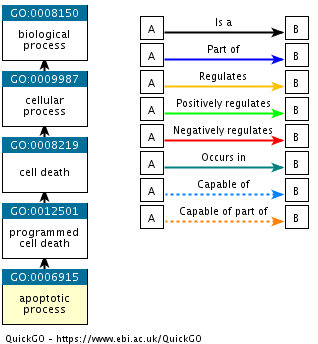
\includegraphics[width=4.42in]{images/go_apoptosis_tree} 

}

\caption{Subárbol de Gene Ontology, donde se presenta el término ``apoptosis'' (apoptotic process) y sus términos ancestros. Imagen extraída de \url{https://www.ebi.ac.uk/QuickGO/term/GO:0006915}.}\label{fig:goApopttree}
\end{figure}


El vocabulario de GO está diseñado para ser agnóstico a las especies, e incluye términos aplicables a procariotas, eucariotas, organismos unicelulares y multicelulares. Las revisiones continuas de la ontología están a cargo de un equipo de editores de ontología con amplia experiencia en biología y representación de conocimientos computacionales.

\hypertarget{otras-ontologias}{%
\subsection{Otras ontologías}\label{otras-ontologias}}

Si bien en la presente tesis se analizó la ontología GO, existen cientos de otras ontologías que pueden ser indagadas mediante AF. Entre estas otras ontologías existentes, debido a su gran popularidad en la comunidad científica, vale la pena mencionar:

\hypertarget{kegg}{%
\subsubsection{KEGG}\label{kegg}}

La ontología provista por el KEGG (Kanehisa \& Goto, 2000) contiene, para cada término o vía metabólica, además de los genes que lo influencian, un diagrama visual que representa el conocimiento experimental sobre el mismo y varias otras funciones que interactúan. Cada diagrama contiene una red de interacciones y reacciones moleculares y está diseñado para vincular los genes del genoma con los productos génicos (principalmente proteínas) de la vía. Esto ha permitido examinar qué vías y funciones asociadas, es probable que estén codificadas en el genoma.

\par

Ejemplos de términos presentes en esta ontología son ``apoptosis'' o ``ciclo celular'' (Figura \ref{fig:keggCellCyclePathw}). En estos diagramas se identifican tres tipos de elementos: cajas rectangulares para representar productos de genes, flechas para el flujo de las reacciones, y cajas con bordes redondeados para vincular a otras vías involucradas en el proceso. A su vez, esta base de datos se complementa con un conjunto de tablas de grupos ortólogos, donde se encuentra la información de subvías conservadas, que son especialmente útiles para la predicción de funciones de genes.
\begin{figure}

{\centering 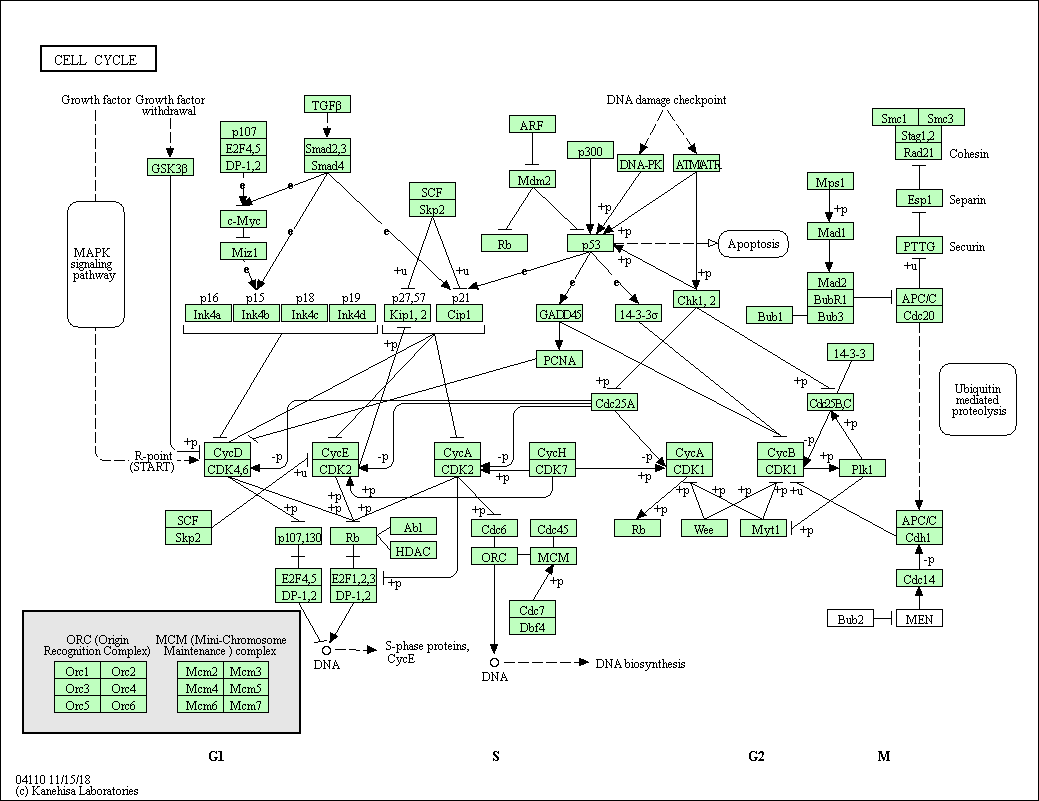
\includegraphics[width=1\linewidth]{images/kegg_cell_cycle_pathway} 

}

\caption{Diagrama de KEGG del ``ciclo celular'' (cell cycle). Imagen extraída de \url{www.genome.jp/kegg-bin/show_pathway?hsa04110}.}\label{fig:keggCellCyclePathw}
\end{figure}


\par

Según los desarrolladores, es una ``representación informática'' del sistema biológico, formada por bloques de construcción y diagramas de cableado, más específicamente, bloques de construcción de genes o proteínas, bloques de construcción de químicos de pequeñas moléculas y reacciones, y diagramas de cableado de interacción molecular y redes de reacción.

\hypertarget{biocarta}{%
\subsubsection{BioCarta}\label{biocarta}}

BioCarta (Nishimura, 2001) fue creado por un grupo de científicos e ingenieros que reconocieron las limitaciones y obsolescencia de la literatura científica de la época. Es muy similar a la ontología del KEGG en el sentido que cada conjunto de genes viene acompañado de un diagrama de las interacciones. Sin embargo, en esta ontología, los diagramas presentan un mayor detalle gráfico como se puede observar en la Figura \ref{fig:biocartaCorticosPathw}, donde se presenta el diagrama del término ``corticosteroides y cardioprotección''.
\begin{figure}

{\centering 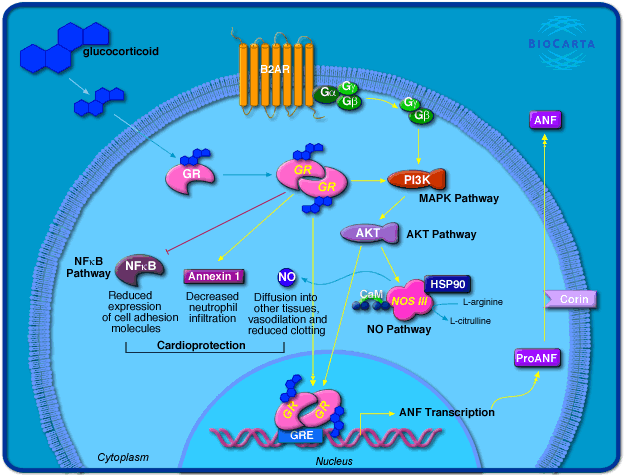
\includegraphics[width=1\linewidth]{images/biocarta_corticosteroids_pathway} 

}

\caption{Diagrama de BioCarta del término ``corticosteroides y cardioprotección''. Imagen extraída de \url{https://david.ncifcrf.gov/biocarta.jsp?path=h_gcrPathway$Corticosteroids+and+cardioprotection\&termId=30000124}.}\label{fig:biocartaCorticosPathw}
\end{figure}


\par

La principal diferencia de BioCarta con KEGG, es que BioCarta fue diseñado para proporcionar un foro para la difusión de información, así como para promover la colaboración entre investigadores, educadores y estudiantes. BioCarta alienta a los científicos a contribuir con contenidos relacionados con sus áreas específicas de especialización. De esta manera, se espera que la contribución de un gran número de especialistas en ciencias de la vida en muchos campos diferentes permita la construcción de modelos detallados y precisos de las interacciones de los productos génicos que superen los esfuerzos de un solo grupo.

\hypertarget{reactome}{%
\subsubsection{Reactome}\label{reactome}}

Reactome: una base de datos de reacciones, vías y procesos biológicos. Reactome (Joshi-Tope et al., 2005) está desarrollado por biólogos expertos, en colaboración con un equipo editorial, todos ellos biólogos con nivel de doctorado. El contenido tiene referencias cruzadas a muchas bases de datos bioinformáticas. El objetivo principal de Reactome es representar visualmente las vías biológicas con todo detalle mecanicista, a la vez que se ponen a disposición los datos de la fuente en un formato computacionalmente accesible.

\par

La unidad central del modelo de datos de Reactome es la reacción. Las entidades (genes, proteínas, complejos y pequeñas moléculas) que participan en las reacciones forman una red de interacciones biológicas y se agrupan en vías. Ejemplos de vías biológicas en Reactome incluyen la ``función inmune innata y adquirida'', la ``regulación transcripcional'', y como se detalla en la Figura \ref{fig:reactomeApoptPathw}, la ``apoptosis''.
\begin{figure}

{\centering 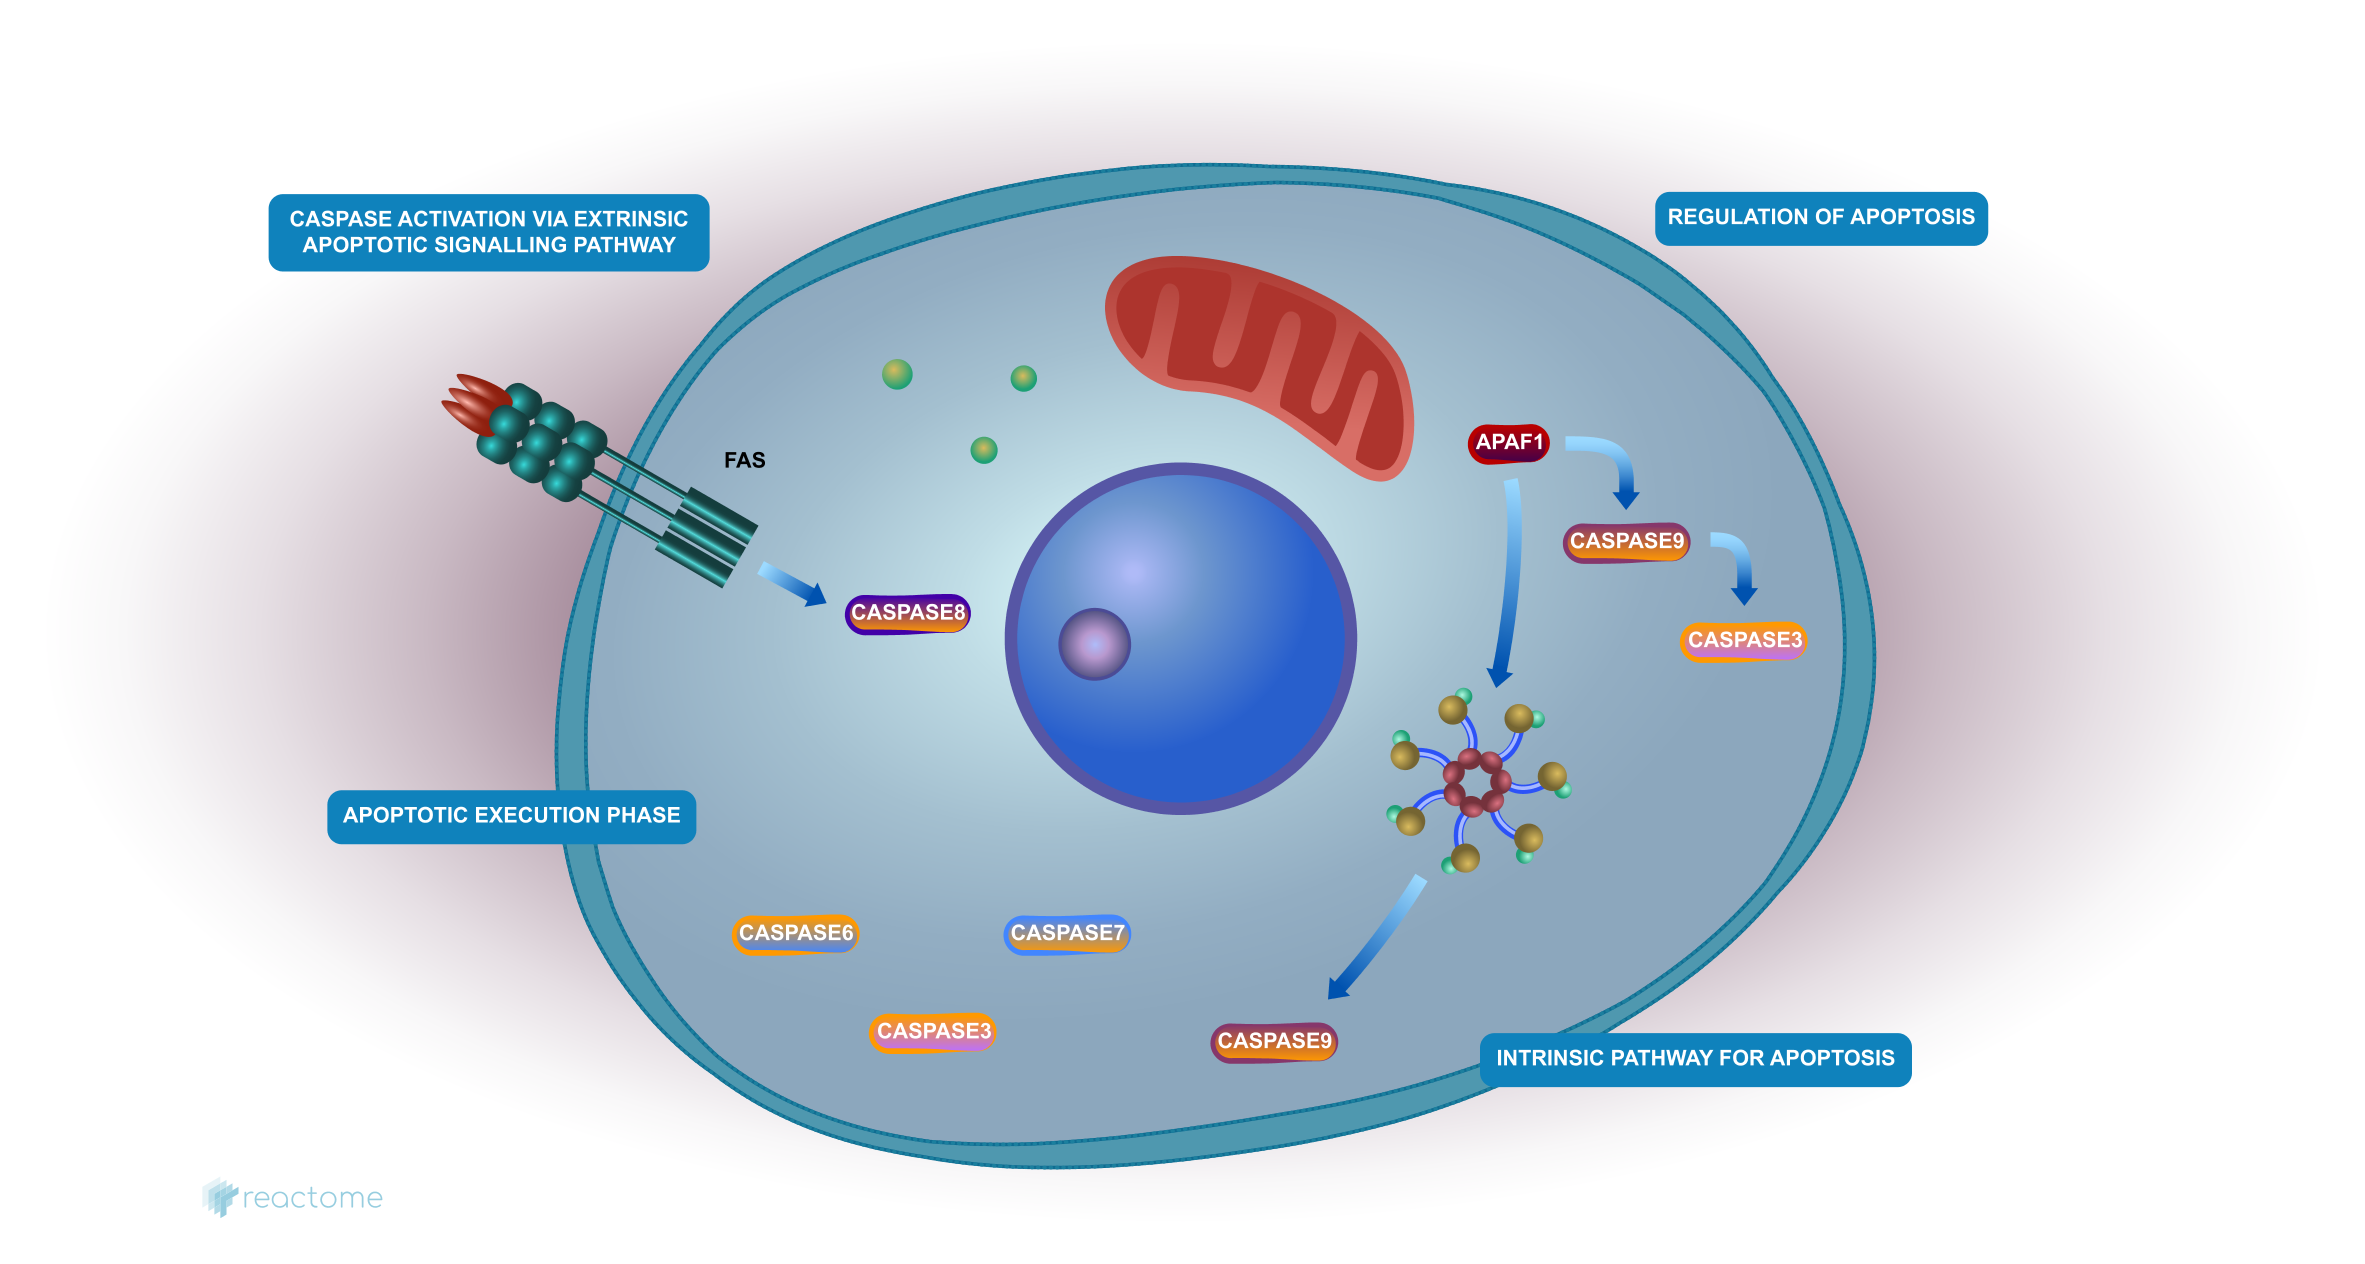
\includegraphics[width=1\linewidth]{images/reactome_apoptosis} 

}

\caption{Diagrama de Reactome del término ``apoptosis''. Imagen extraída de \url{https://www.reactome.org/content/detail/R-HSA-109581}.}\label{fig:reactomeApoptPathw}
\end{figure}


\par

Las vías representadas en Reactome son específicas para cada especie, y cada paso de la vía está respaldado por citas bibliográficas que contienen una verificación experimental del proceso representado. Si no existe una verificación experimental, las vías pueden contener pasos inferidos, pero sólo si un biólogo experto, nombrado como \emph{autor de la vía}, y un segundo biólogo, nombrado como \emph{revisor}, están de acuerdo en que esto es una inferencia válida a hacer. Las vías humanas se utilizan para generar computacionalmente, mediante un proceso basado en la ortología, las vías derivadas de otros organismos.

\hypertarget{msigdb}{%
\subsubsection{MSigDB}\label{msigdb}}

MSigDB (Liberzon et al., 2011) es la ontología desarrollada por el Broad Institute (\url{https://www.broadinstitute.org/}), esta ontología es un compilado de ciertos conjuntos de genes provenientes de otras ontologías, entre ellas las descriptas previamente. MSigDB agrupa todos sus conjuntos de genes dentro de ocho categorías:
\begin{itemize}
\tightlist
\item
  \textbf{Conjuntos de genes distintivos}: resumen y representan estados o procesos biológicos específicos bien definidos. Estos conjuntos de genes fueron generados por una metodología computacional basada en la identificación de superposiciones entre conjuntos de genes en MSigDB y la retención de genes que muestran detalles de expresión coordinada.
\item
  \textbf{Conjuntos de genes posicionales}: correspondientes a cada cromosoma humano y a cada banda citogenética que tenga al menos un gen.
\item
  \textbf{Conjuntos de genes curados}: obtenidos y curados a partir de diversas fuentes, como bases de datos de ontologías (KEGG, BioCarta y Reactome), literatura biomédica y el conocimiento de expertos en la materia.
\item
  \textbf{Conjuntos de genes del motivo}: representan objetivos potenciales de regulación por factores de transcripción o microARNs. Los conjuntos consisten en genes agrupados por contener motivos de secuencia corta en común, pertenecientes a regiones codificadoras no proteicas. Los motivos representan elementos de regulación cis conocidos o probables en promotores y 3'-UTRs.
\item
  \textbf{Conjuntos de genes computacionales}: definidos por la minería de grandes colecciones de datos orientados al cáncer.
\item
  \textbf{Conjuntos de genes de GO}: contienen conjuntos de genes seleccionados de GO.
\item
  \textbf{Firmas oncogénicas}: representan firmas de vías celulares que a menudo están desreguladas en el cáncer. La mayoría de las firmas se generaron directamente a partir de datos de genes que implicaban la perturbación de genes cancerígenos conocidos.
\item
  \textbf{Firmas inmunológicas}: representan estados celulares y perturbaciones dentro del sistema inmunológico. Las firmas fueron generadas por la curación manual de estudios publicados en inmunología humana y de ratones.
\end{itemize}
\hypertarget{sec:af}{%
\section{Metodologías de Análisis Funcional (AF)}\label{sec:af}}

El análisis funcional refiere a técnicas que permiten, dado un experimento, evaluar el impacto de la interacción de grupos de genes sobre características biológicas. Partiendo de una matriz de expresión de genes con muestras pertenecientes a una de dos condiciones, los algoritmos de AF buscan detectar aquellos términos biológicos que se encuentran desregulados entre ambas condiciones. Una vez determinada la base de datos ontológica de interés, el investigador debe seleccionar cuál técnica de AF utilizar.

\par

Se diferencian dos categorías de algoritmos para llevar a cabo el AF (D. W. Huang et al., 2008a). La principal diferencia entre estas categorías es la estrategia que llevan a cabo para el análisis:

\hypertarget{sec:asr}{%
\subsection{Análisis de Sobre-Representación (ASR)}\label{sec:asr}}

Esta metodología requiere definir la lista de genes de interés o \textbf{candidatos}, generalmente aquellos que se encuentran diferencialmente expresados en el experimento, es decir, un vector con los nombres de los genes. Adicionalmente requiere de una segunda lista de genes, que utiliza para especificar lo que es esperable como comportamiento de \textbf{referencia} del modelo biológico, generalmente todos los genes presentes en el experimento. Luego, para cada término, realiza de forma independiente un test de hipótesis comparando las proporciones observadas sobre los candidatos con respecto a la referencia. De este modo, para cada término se obtiene un p-valor asociado que denota si existe evidencia de que las proporciones son diferentes.

\par

En la Figura \ref{fig:diagramaORA} se puede apreciar un diagrama de lo que sería el proceso completo para llevar a cabo un ASR. De este diagrama se desprenden varios aspectos que resultan variables. Diversos autores han propuesto diferentes test de hipótesis (Falcon \& Gentleman, 2006; Fang \& Gough, 2014; Fresno \& Fernández, 2013; D. W. Huang et al., 2008b), y principalmente de allí es que surgen grandes cantidades de alternativas de ASR. Más aún, la elección de la lista de referencia no queda del todo clara, y se desprenden dos sugerencias con gran validez estadística: utilizar todos los genes del experimento (como en la Figura \ref{fig:diagramaORA}), o utilizar todo el genoma de la especie en cuestión (Fresno et al., 2012).

\newpage
\begin{figure}

{\centering 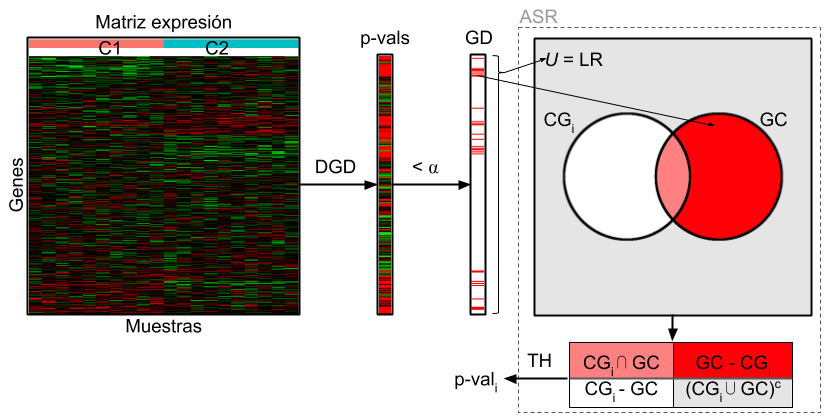
\includegraphics[width=1\linewidth]{images/diagrama_ORA} 

}

\caption{Diagrama clásico del proceso completo de Análisis de Sobre-Representación (ASR). Este proceso parte de una Matriz de expresión, con Genes en filas y Muestras en columnas, y la etiqueta de condición de cada muestra (C1 y C2). Mediante un algoritmo de Detección de Genes Diferenciales (DGD) se obtiene para cada gen un p-valor asociado (p-vals). Aplicando un nivel de corte \(\alpha\) a estos p-valores (\(< \alpha\)), se obtiene cuáles son Genes Diferenciales (GD) y cuáles no. Aquí es donde efectivamente comienza el ASR, los algoritmos de ASR requieren de dos listas: la de genes candidatos (usualmente los GD), y la Lista de Referencia (LR; usualmente todos los genes detectados en el experimento). A partir de estas listas de genes, para cada Conjunto de Genes (CG\(_i\)) se genera una tabla de contingencia, a la cual se le aplica un Test de Hipótesis (TH) del cual resulta un p-valor asociado al CG\(_i\) (p-val\(_i\)).}\label{fig:diagramaORA}
\end{figure}


\hypertarget{puntuacion-funcional-de-clase-pfc}{%
\subsection{Puntuación Funcional de Clase (PFC)}\label{puntuacion-funcional-de-clase-pfc}}

Esta metodología construye un ordenamiento de los genes a partir de la totalidad del perfil de expresión. El objetivo es determinar si todos los miembros de una característica biológica de interés, están distribuidos aleatoriamente o no (en algún extremo) a lo largo del ordenamiento generado (Subramanian et al., 2005). Para ello, los genes se organizan mediante algún criterio de ordenamiento que refleje la diferencia entre ambas condiciones bajo estudio, por ejemplo, para cada gen obtener la diferencia de medias entre ambas condiciones. Luego, para un término biológico en particular, se recorre este ordenamiento para calcular el máximo del enriquecimiento inducido, lo cual se conoce como \textbf{Enrichment Score} (ES) del término. Para ello, a cada gen se le aplica una función de coste que aumenta (o disminuye) proporcionalmente a la correlación de su nivel de expresión con el fenotipo de las condiciones, cada vez que encuentra un gen que pertenece (o no) a la lista de miembros de la categoría de interés. Este ES se compara con la distribución nula generada por las permutaciones en las etiquetas de las condiciones, con el fin de evaluar si el ordenamiento original es esperable o generado por azar. En caso de que difiera del azar, existen diferentes criterios para definir, para el experimento dado, cuáles son los genes más influyentes en el término. Normalmente se utilizan los genes más cercanos al máximo del ES, o los genes pertenecientes al segmento más pequeño entre el coste máximo y el principio o el final de la lista ordenada.

\par

En la Figura \ref{fig:diagramaFCS} se observa el diagrama de lo que sería un proceso completo de PFC. De este diagrama, diversos aspectos difieren dependiendo del algoritmo de PFC a utilizar. Por ejemplo, ciertos algoritmos sugieren hacer permutación en las etiquetas de los genes, otros en las etiquetas de las muestras, y finalmente otros, en las etiquetas de genes del ordenamiento generado. Más aún, la principal diferencia entre uno y otro algoritmo de PFC reside en la función de ES, si bien la idea por detrás resulta similar, las ponderaciones de cada gen varían. Finalmente, vale la pena mencionar que ciertos algoritmos fijan diferentes filtros de los conjuntos de genes a analizar ya que suponen que fuera de esos límites el algoritmo pierde potencia estadística.
\begin{figure}

{\centering 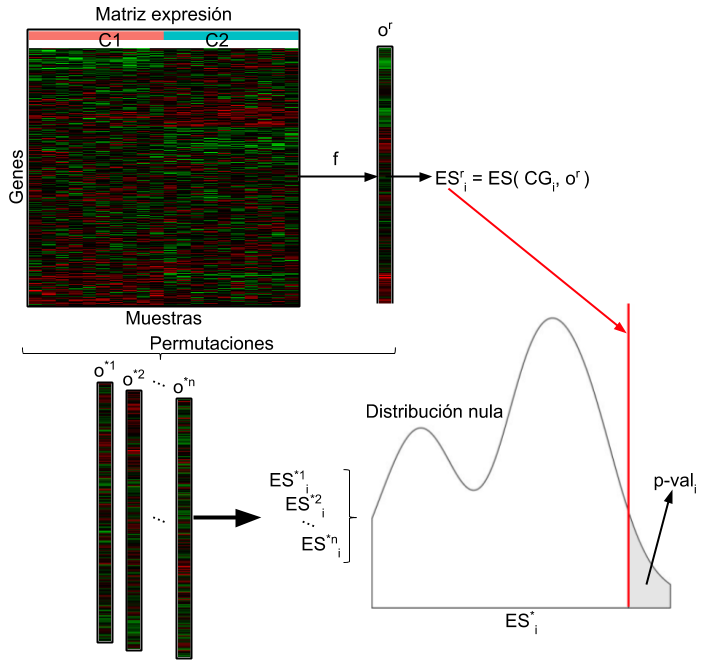
\includegraphics[width=1\linewidth]{images/diagrama_FCS} 

}

\caption{Diagrama clásico del proceso completo de Puntuación Funcional de Clase (PFC). Este proceso parte de una Matriz de expresión, con Genes en filas y Muestras en columnas, y la etiqueta de de condición de cada muestra (C1 y C2). Mediante alguna función particular (f) se obtiene un ordenamiento real (o\(^r\)) para los genes, es decir, para cada gen un valor numérico que le asigna una posición de orden. Luego, mediante una función llamada Enrichment Score (ES), partiendo de un conjunto de genes particular (CG\(_i\)) y el ordenamiento, se obtiene un valor de enriquecimiento real para el conjunto de genes (ES\(^r_i\)). Esta función ES es diferente dependiendo del algoritmo de PFC utilizado. Luego, mediante permutaciones sobre las condiciones, las etiquetas de los genes, ó del ordenamiento, se generan nuevos vectores de ordenamiento (o\(^*_1\), o\(^*_2\), \ldots{}, o\(^*_n\)). Con cada uno de estos ordenamientos permutados, se genera un valor de enriquecimiento permutado para el conjunto de genes (ES\(^{*1}_i\), ES\(^{*2}_i\), \ldots{}, ES\(^{*n}_i\)). Dado que se cuenta con n muestras permutadas de valores de enriquecimiento, se procede a realizar una distribución nula, con la cual se compara contra el valor de enriquecimiento real ES\(^r_i\), y por ende se obtiene un p-valor asociado al conjunto de genes dado (p-val\(_i\)).}\label{fig:diagramaFCS}
\end{figure}


\hypertarget{analisis-de-enriquecimiento-modular}{%
\subsection{Análisis de Enriquecimiento Modular}\label{analisis-de-enriquecimiento-modular}}

Vale la pena mencionar que en la literatura se suele encontrar una tercer alternativa de AF, llamada Análisis de Enriquecimiento Modular. Esta metodología requiere, adicionalmente, que los CG presenten alguna relación entre ellos. En la presente tesis no se tiene en cuenta esta metodología ya que en el común de las bases de datos de CG no existe relación entre sus términos, lo cual resulta en un gran limitante para el análisis.

\hypertarget{comentarios-finales}{%
\section{Comentarios finales}\label{comentarios-finales}}

Tanto el ASR como PFC se utilizan para saber si un término se enriquece (o no) en la comparación de las condiciones estudiadas. Sin embargo, la formulación del problema es diferente para cada caso. Para realizar el análisis a través del ASR es necesario proporcionar dos listas, una de ellas de referencia y la otra de los genes candidatos. Este último suele estar formado por aquellos genes que se han identificado como expresados de forma diferencial entre dos condiciones experimentales (por ejemplo, tumor vs.~normal) para un umbral definido. En PFC, se utiliza una matriz de expresión única que contiene todos los genes detectados por el experimento y, a continuación, se utiliza el criterio de ordenación propuesto para medir el enriquecimiento. En este sentido, PFC en comparación al ASR, no utiliza un umbral para definir la lista de candidatos, y por ende PFC utiliza toda la información presente en el experimento.

\par

Si bien, existen principalmente dos metodologías para realizar el AF, tanto para ASR como para PFC, existen grandes cantidades de diferentes algoritmos desarrollados, cada uno con sus propios supuestos, test, y parametrizaciones. En este sentido, no fue evaluado qué beneficios trae un algoritmo frente al resto. Por consiguiente, para el investigador, la elección del algoritmo de AF a utilizar termina siendo más una cuestión de elección aleatoria, que una elección adaptada al experimento en cuestión, de la hipótesis bajo estudio, o del enfoque de la investigación.

\hypertarget{cap:ngs}{%
\chapter{Fuentes de datos biológicas}\label{cap:ngs}}

La célula es la unidad estructural, funcional y biológica básica de todos los organismos vivos conocidos. Los organismos pueden clasificarse como unicelulares (compuestos de una sola célula, incluidas las bacterias) ó multicelulares (incluidas las plantas y los animales). Existen dos tipos de células, las eucariotas, que contienen núcleo celular, y las procariotas, que no lo contienen.

Las células eucariotas están compuestas por diversos orgánulos como la membrana, el citoplasma y el núcleo (Figura \ref{fig:cell}). La membrana envuelve y protege a la célula, y regula lo que entra y sale (selectivamente permeable). Dentro de la membrana, el citoplasma ocupa la mayor parte del volumen de la célula, y la separa del núcleo celular. El más prominente de los orgánulos es el núcleo celular, el cual aloja el material genético de la célula. El material genético se presenta como Acido DesoxirriboNucleico (ADN), el cual está organizado en una o más moléculas, llamadas cromosomas.
\begin{figure}

{\centering 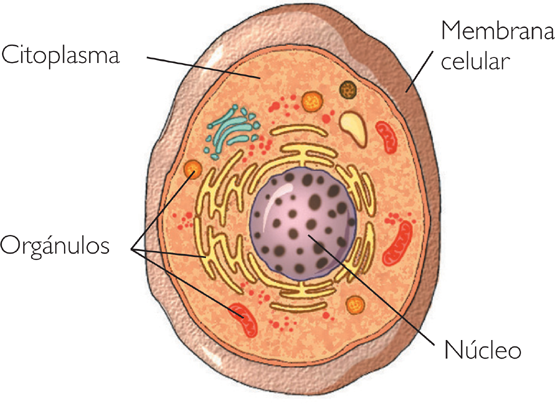
\includegraphics[width=0.7\linewidth]{images/celula} 

}

\caption{Diagrama simplificado de una célula eucariota. Imagen extraída de \url{https://biologiarubenurjc.wordpress.com/2012/03/19/membrana-nucleo-y-citoplasma/}.}\label{fig:cell}
\end{figure}


La información biológica contenida en un organismo está codificada en su secuencia de ADN. El ácido desoxirribonucleico esta organizado en dos cadenas que se enrollan una alrededor de la otra para formar una doble hélice (Figura \ref{fig:adn}) que lleva las instrucciones genéticas utilizadas en el crecimiento, desarrollo, funcionamiento y reproducción de todos los organismos conocidos. El ADN esta conformado por unidades más pequeñas conocidas como nucleótidos. Cada nucleótido está compuesto por un azúcar llamado desoxirribosa, un grupo de fosfatos, y por una de cuatro bases nitrogenadas que son la citosina (C), guanina (G), adenina (A) ó timina (T). Los nucleótidos están unidos entre sí en una cadena por enlaces covalentes entre el azúcar de un nucleótido y el fosfato del siguiente. Las bases nitrogenadas de las dos cadenas de nucleótidos separadas se unen, según las reglas de emparejamiento de bases (A con T y C con G). Ambas cadenas de ADN almacenan la misma información biológica. Las regiones relevantes del ADN se encuentran localizadas en los cromosomas y se denominan genes. Si bien la cadena de ADN contiene millones de nucleótidos, solo un pequeño porcentaje de ella codifica proteínas (alrededor del 2\% para los humanos).
\begin{figure}

{\centering 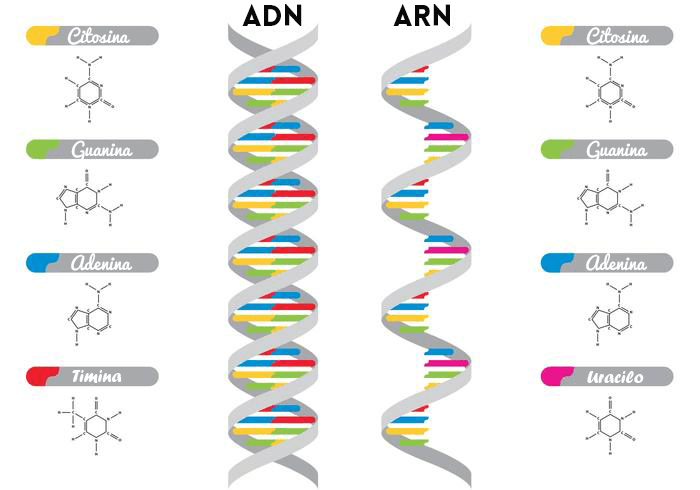
\includegraphics[width=0.7\linewidth]{images/ADN_ARN} 

}

\caption{Diagrama de la estructura del ADN y ARN. Imagen extraída de \url{https://diferencias-entre.org/diferencias-entre-adn-y-arn/}.}\label{fig:adn}
\end{figure}


Las células utilizan el ADN para el almacenamiento de información a largo plazo. Por otra parte, para las demás tareas en que sea necesaria la información genética, las células utilizan el Ácido RiboNucleico (ARN). El ARN se obtiene a partir del ADN para llevar a cabo tareas celulares como la síntesis de proteínas, las cuales son cadenas de aminoácidos que tienen funcionalidades básicas tanto para el metabolismo como para la fisiología celular y, en consecuencia, del organismo. La decodificación del material genético comienza dentro del núcleo celular, donde las hebras de ARN se crean utilizando el ADN como plantilla en un proceso llamado transcripción. Al igual que el ADN, el ARN se ensambla como una cadena de nucleótidos, pero a diferencia del ADN, se encuentra como una única hebra (Figura \ref{fig:adn}), donde las bases timina son reemplazadas por uracilo (U).

Los organismos celulares utilizan ARN mensajero (ARNm) para transmitir información genética. Orgánulos llamados ribosomas procesan el ARNm tomando cada combinación de tres nucleótidos para codificar cada uno de los 20 aminoácidos posibles. Posteriormente, los ribosomas generan la cadena de aminoácidos decodificados y así conforman la proteína codificada.

De los resultados de estos procesos celulares, existen diversos aspectos biológicos de interés científico: el genoma, el proteoma, el metaboloma, entre otros, los cuales se conocen como las diversas fuentes ómicas. A partir de una muestra biológica, para cada fuente ómica, existen tecnologías capaces de medir sus niveles de expresión. Es decir, para una misma muestra es posible obtener niveles de expresión tanto de genes, proteínas, etc.

En la presente tesis nos centraremos únicamente en aquellas ómicas que permitan obtener sus niveles de expresión en forma de matriz. Por ejemplo, en genómica, al secuenciar \emph{m} muestras, es posible obtener una matriz \(G_{g*m}\), con expresión obtenida para \emph{g} genes, donde \(G[i,j]\) será un valor numérico representando el nivel de expresión del \emph{i-ésimo} gen para la \emph{j-ésima} muestra.

\hypertarget{sec:technols}{%
\section{Tecnologías de obtención de expresión biológica}\label{sec:technols}}

La presente sección tiene como objetivo mencionar brevemente aspectos pertinentes sobre las tecnologías mediante las cuales se obtienen los niveles de expresión de las ómicas analizadas en la tesis.

\hypertarget{microarreglos-de-adn}{%
\subsection{Microarreglos de ADN}\label{microarreglos-de-adn}}

Un microarreglo es una superficie sólida donde pequeños fragmentos de ADN (sondas) son dispuestos en forma de matriz bidimensional. Cada celda contiene secuencias de ADN correspondientes a \textbf{genes}, ligados químicamente en cada celda. Para medir la expresión génica se extrae ARNm de muestras biológicas, este ARNm es luego copiado (transcripción reversa) obteniendo como resultado ADN complementario o ADNc. A este último se lo amplifica incorporando moléculas fluorescentes en las réplicas. Las copias fluorescentes del ADNc se vuelcan luego, sobre el microarreglo. De esta manera, las secuencias marcadas con moléculas fluorescentes se hibridizan (se ``pegan'') a su cadena complementaria presente en el microarreglo. Luego, el microarreglo se escanea excitando las celdas con un láser y midiendo la intensidad de luz emitida por las moléculas fluorescentes. El resultado de escanear un microarreglo es una imagen por cada microarreglo. La intensidad medida en cada celda es, en principio, proporcional a la cantidad de ARNm, específico para esa celda, presente en la muestra biológica (Fernández, Alvarez, Podhajcer, \& Stolovitzky, 2007).

\par

Las imágenes resultantes del escaneo son procesadas por programas informáticos que identifican las celdas del microarreglo y miden la intensidad de luz registrada. Como resultado del procesamiento de la imagen se obtiene una serie de datos por cada celda perteneciente a cada microarreglo. En particular se obtienen los valores de intensidad de la celda, de la intensidad que rodea a la celda (intensidad de fondo), algunos índices que aportan información sobre las características de la celda (por ejemplo, el área y el perímetro de la misma) y la distribución de las intensidades dentro de cada celda. Toda esta información se utiliza para determinar la calidad del escaneo (Fresno et al., 2014). Una vez eliminadas aquellas celdas defectuosas o que presentan niveles de calidad de señal inadecuados, se normalizan los valores, comúnmente aplicando logaritmo. Finalmente se obtiene como resultado un archivo con la intensidad o el nivel de expresión de cada celda o gen.

\par

Luego de procesar los archivos resultantes de microarreglos, y repetir el procedimiento para varios sujetos, se llega a una matriz de expresión con genes en filas y sujetos en columnas. Cada valor de la matriz representa la intensidad o nivel de expresión de un gen para una muestra. Luego de una correcta normalización de esta matriz, se llega a una del estilo a la que se muestra a continuación; sub-matriz de \(6\times5\) de datos reales provenientes de microarreglos de ADN:

\newpage
\begin{verbatim}
        A2-A0CM-01A A2-A0D0-01A A2-A0D1-01A A2-A0D2-01A A2-A0EQ-01A
ZBTB16  -0.12125000     0.00425    -0.98975  3.31300000   0.5387500
DNAJB13 -0.48200000    -0.53250    -0.60450 -0.61750000  -0.2670000
SFRP5   -0.02033333     0.22900     0.28440 -0.03216667  -0.3128333
RRAGC    1.23525000     0.68625     0.89750  1.71275000   0.9832500
IAPP     0.11500000     0.06250     1.26450  0.43500000   1.0490000
ELMO1    0.19487500    -0.35275    -0.66825  0.36437500   0.6860000
\end{verbatim}
Dado que los valores de expresión provienen de niveles de intensidad de luz, los datos son valores continuos. Por ende, es de esperar que la distribución de los genes, para cada sujeto, se asemeje a una distribución \(Normal\), como se observa en la Figura \ref{fig:maDens}.
\begin{figure}

{\centering 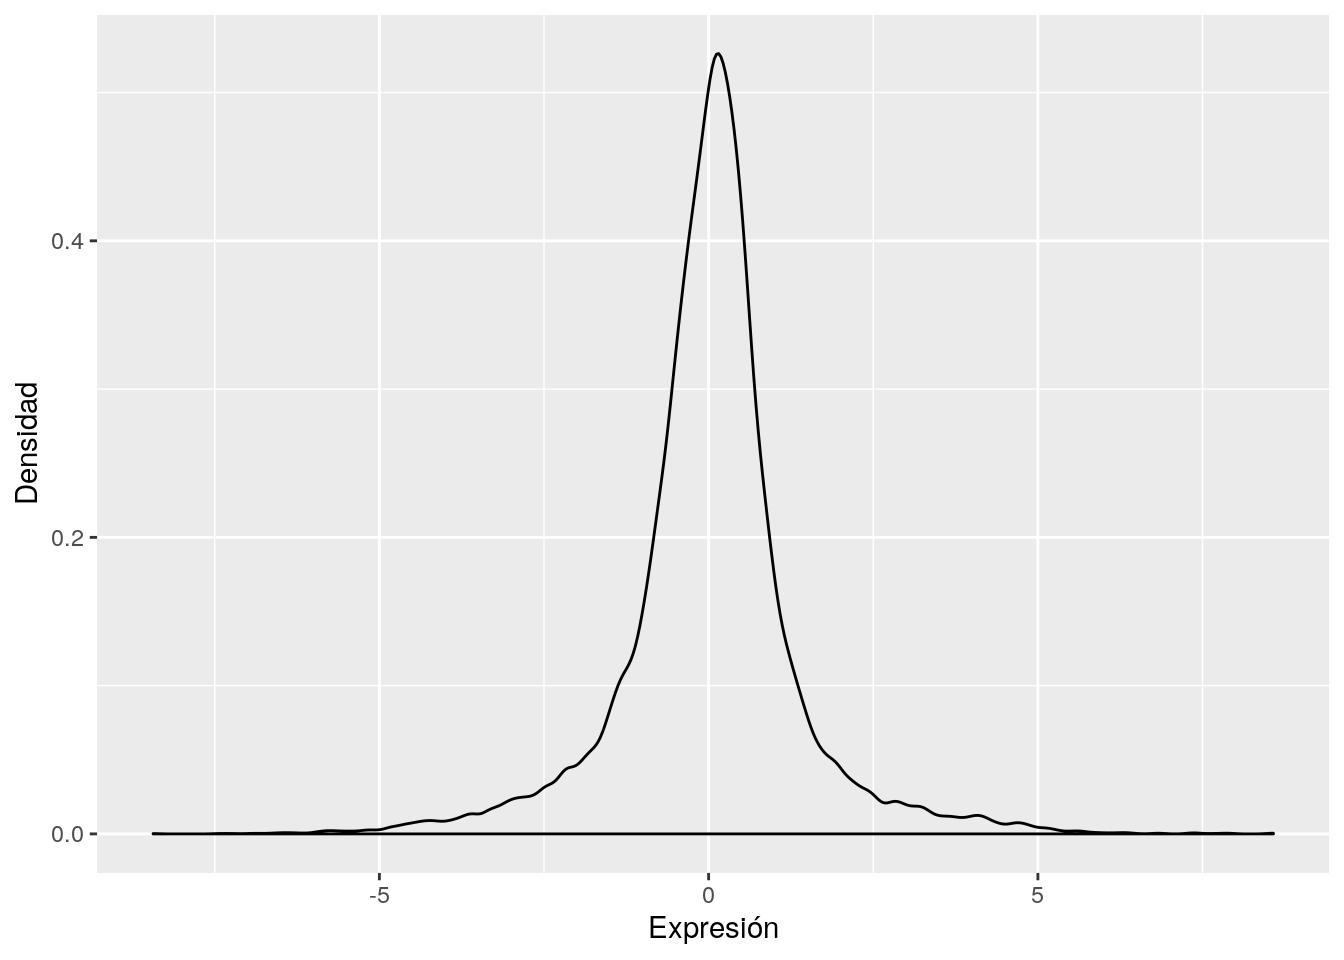
\includegraphics[width=0.7\linewidth]{02_fuentes_datos_files/figure-latex/maDens-1} 

}

\caption{Densidad de los valores de expresión de los genes de un sujeto, para datos obtenidos mediante Microarreglos de ADN.}\label{fig:maDens}
\end{figure}
\hypertarget{itraq}{%
\subsection{iTRAQ}\label{itraq}}

El método iTRAQ se basa en el marcado químico, con etiquetas de masa variable, de las aminas de los péptidos de las digestiones de \textbf{proteínas} presentes en una muestra biológica. Actualmente hay dos reactivos utilizados principalmente, que pueden usarse para marcar todos los péptidos de diferentes muestras. Estas muestras luego se agrupan y generalmente se fraccionan mediante cromatografía líquida, y se analizan mediante espectrometría de masas en tándem. Luego se realiza una búsqueda en la base de datos utilizando los datos de fragmentación para identificar los péptidos marcados y, por lo tanto, las proteínas correspondientes. La fragmentación de la etiqueta adjunta genera un ión indicador de baja masa molecular que se puede usar para cuantificar relativamente los péptidos y las proteínas a partir de las cuales se originaron.

\par

A nivel peptídico, las señales de los iones indicadores de cada espectro permiten calcular la abundancia relativa (ratio) de los péptidos identificados por este espectro. Las proporciones combinadas de los péptidos de una proteína representan la cuantificación relativa de esa proteína. De esta manera se obtiene una matriz resultante de proteínas \(\times\) sujetos, con valores del ratio de la expresión de una proteína para un sujeto dado. Si bien la matriz esta indexada a nivel de proteínas, resulta de mayor interés estudiarla a nivel de genes, por ello, consultando bases de datos de anotación, se traduce cada proteína al gen que la produce. Luego de una normalización adecuada se obtiene una matriz como la que se presenta:
\begin{verbatim}
      A2-A0CM-01A A2-A0D0-01A A2-A0D1-01A  A2-A0D2-01A A2-A0EQ-01A
RRAGC  0.17794796  0.27751403 -0.13956920  0.098823426  -0.1745463
ELMO1  0.39888804  0.30589111 -0.09178467 -0.126851824   0.7252130
BAX    0.35139262  0.08414816  0.23821506 -0.118018092  -0.1782356
PDCD4  0.04627689  0.02277544  0.65416083 -0.353588366  -0.3033616
PDCD2 -0.19497549  0.55829865 -0.15272404 -0.024984301   0.6028903
PTPN6  0.17697246  0.19056327 -0.38121552 -0.002048376   0.8563106
\end{verbatim}
Dado que los valores de expresión provienen de niveles de señales, los datos son valores continuos. Por ende, es de esperar que la distribución se asemeje a una distribución \(Normal\), como se observa en la Figura \ref{fig:protDens}. Vale la pena aclarar que ya que esta matriz sigue una distribución similar a la obtenida mendiante Microarreglos de ADN, es común que se utilicen los mismos métodos de análisis para ambas fuentes de datos.
\begin{figure}

{\centering 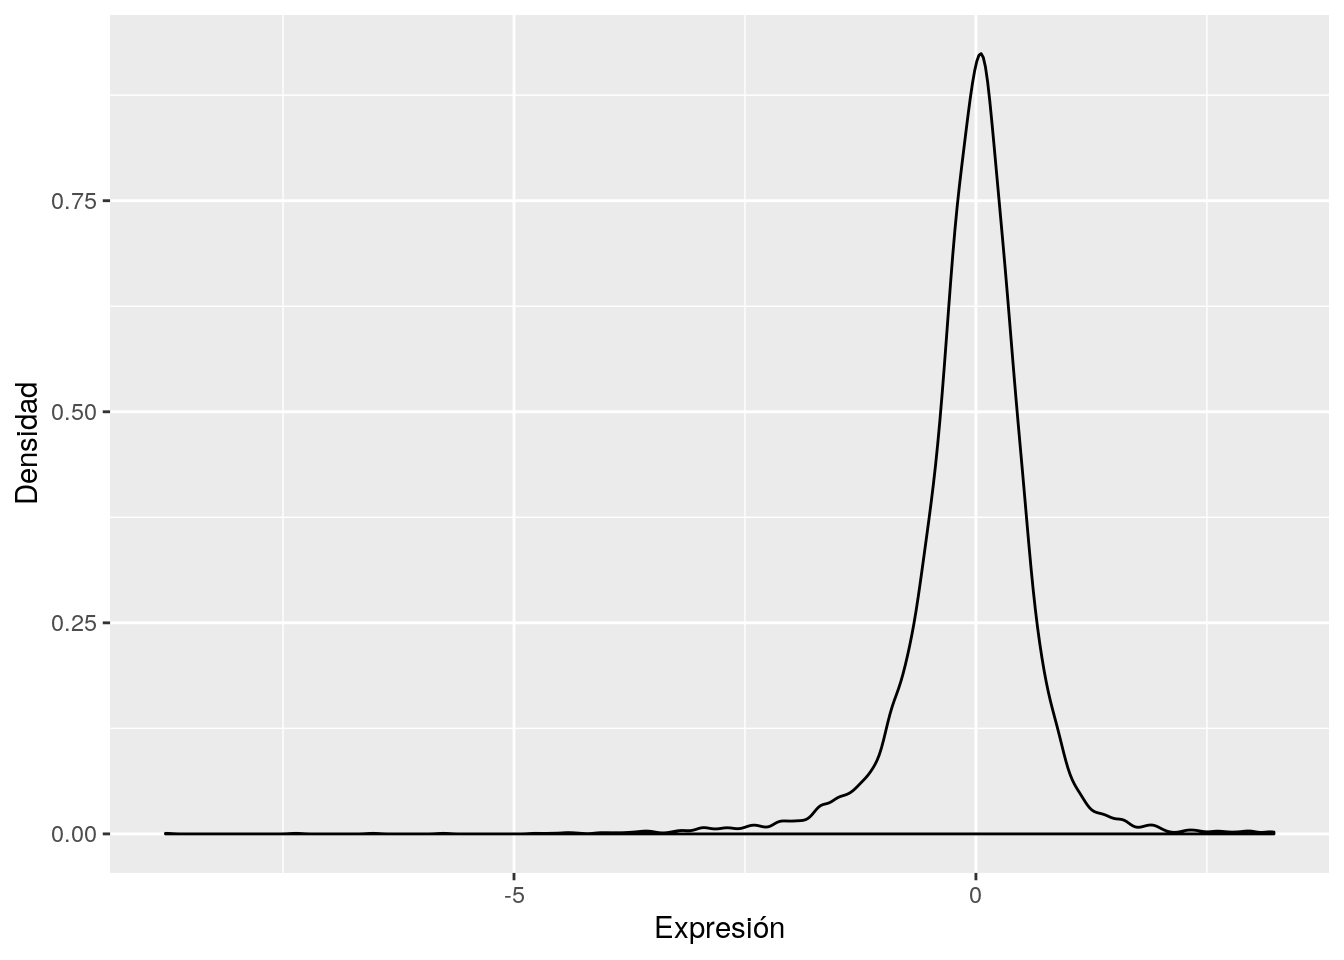
\includegraphics[width=0.7\linewidth]{02_fuentes_datos_files/figure-latex/protDens-1} 

}

\caption{Densidad de los valores de expresión de los genes de un sujeto, para datos obtenidos mediante iTRAQ.}\label{fig:protDens}
\end{figure}
\hypertarget{secuenciacion-de-arn}{%
\subsection{Secuenciación de ARN}\label{secuenciacion-de-arn}}

Este tipo de tecnologías se basa en poder obtener para una muestra biológica, las secuencias de \textbf{nucleótidos} detectadas. En este sentido se obtienen millones de cadenas de nucleótidos, que al mapearlos (unirlos) permiten obtener la cantidad de veces que subcadenas del genoma aparecen en la muestra. Al poseer información a nivel de nucleótidos, surgen ventajas con respecto a los microarreglos de ADN, por ejemplo, poder detectar mutaciones de nucleótidos, e incluso estudiar la muestra a niveles más detallados que genes (transcriptos, exones, intrones, etc.).

\par

Una vez obtenido el ARN de la muestra biológica, se retrotranscribe para obtener ADN complementario (ADNc) a estas cadenas. El proceso siguiente es la fragmentación en donde, mediante cortes en secciones aleatorias, se llevan estas grandes cadenas de ADNc a fragmentos de entre 300 y 1000 nucleótidos. Cada uno de estos fragmentos es posteriormente clonado varias veces, produciendo millones de copias de cada fragmento. Aquí es cuando comienza el proceso de secuenciación propiamente dicho. En el caso de la secuenciación por síntesis, por ejemplo de las plataformas de \emph{Illumina}, los fragmentos de ADNc se ponen en un pool que contiene nucleótidos individuales marcados con fluoróforos, cada una de las cuatro bases con un color diferente. Al entrar en contacto el ADNc con estos nucleótidos libres, se incorporan como hebra complementaria del ADNc, de esta manera se logra incorporar un color a cada una de las bases de los fragmentos de ADNc. Luego, cada fragmento pasa por un sistema que permite leer el color incorporado a cada nucleótido. Es así que traduciendo los colores, se logra detectar los nucleótidos que componen cada fragmento. Al finalizar el proceso de secuenciación de ARN, se cuenta con un archivo con millones de lecturas, una por cada fragmento. Cada lectura se representa con 4 líneas en el archivo, como la que se muestra a continuación:
\begin{verbatim}
@SEQ_ID
GATTTGGGGTTCAAAGCAGTATCGATCAAATAGTAAATCCATTTGTTCAACTCACAGTTT
+
!''*((((***+))%%%++)(%%%%).1***-+*''))**55CCF>>>>>>CCCCCCC65
\end{verbatim}
La primer línea es un identificador de la secuencia, la segunda es la que contiene la secuencia de nucleótidos leídos, la tercera es un campo opcional, y la cuarta es la calidad de lectura de cada nucleótido.

\par

Una vez que se cuenta con el archivo resultante de la secuenciación, comienza el proceso bioinformático en sí. El primer paso consiste en la reconstrucción de los transcriptos de las lecturas para determinar de qué genes proceden. Este paso consiste en mapear las lecturas con el genoma ó transcriptoma respectivo. En términos sencillos, si se piensa en las lecturas como piezas de un rompecabezas, el genoma ó transcriptoma es la imagen que se obtendrá uniendo correctamente las piezas. Para el proceso de mapeado, una alternativa es realizar un ensamblaje de novo para inferir las secuencias de las transcripciones sin usar más información que la contenida en las lecturas. Por otro lado, el conocimiento a priori del genoma o transcriptoma de la especie en estudio se puede utilizar como una referencia que facilitará la reconstrucción, lo cual se conoce como mapeado con referencia. Al final de la etapa de mapeado, se cuenta con información referente a qué gen o transcripto pertenece cada fragmento leído.

\par

Al momento inicial, cuando se obtiene el ARN de la muestra biológica, un gen más activo se encontrará más expresado que el resto, y por consiguiente, el gen presentará mayor cantidad de fragmentos asociados. Para obtener el nivel de expresión de cada gen ó transcripto particular, simplemente se puede tomar la cantidad de fragmentos que fueron mapeados al mismo. De este modo, mediante secuenciación de ARN se permite obtener una matriz de genes \(\times\) sujetos, con un conteo para cada gen y sujeto, como se puede apreciar a continuación:
\begin{verbatim}
        A2-A0CM-01A A2-A0D0-01A A2-A0D1-01A A2-A0D2-01A A2-A0EQ-01A
ZBTB16           89          31         126         449          81
DNAJB13          11          11          44          31          43
SFRP5             1           2           0           0           0
RRAGC          2797        1453        1680        4573        2631
IAPP            162          78         167         151         195
ELMO1          1740         677         540        1758        4204
\end{verbatim}
Dado que los valores de expresión se desprenden de la cantidad de fragmentos mapeados, los datos son valores de conteos (no continuos). Por ende, es de esperar que la distribución de los genes, para cada sujeto, se asemeje a una distribución de \(Poisson\) o \(Binomial Negativa\), como se observa en la Figura \ref{fig:rnaDens}.
\begin{figure}

{\centering 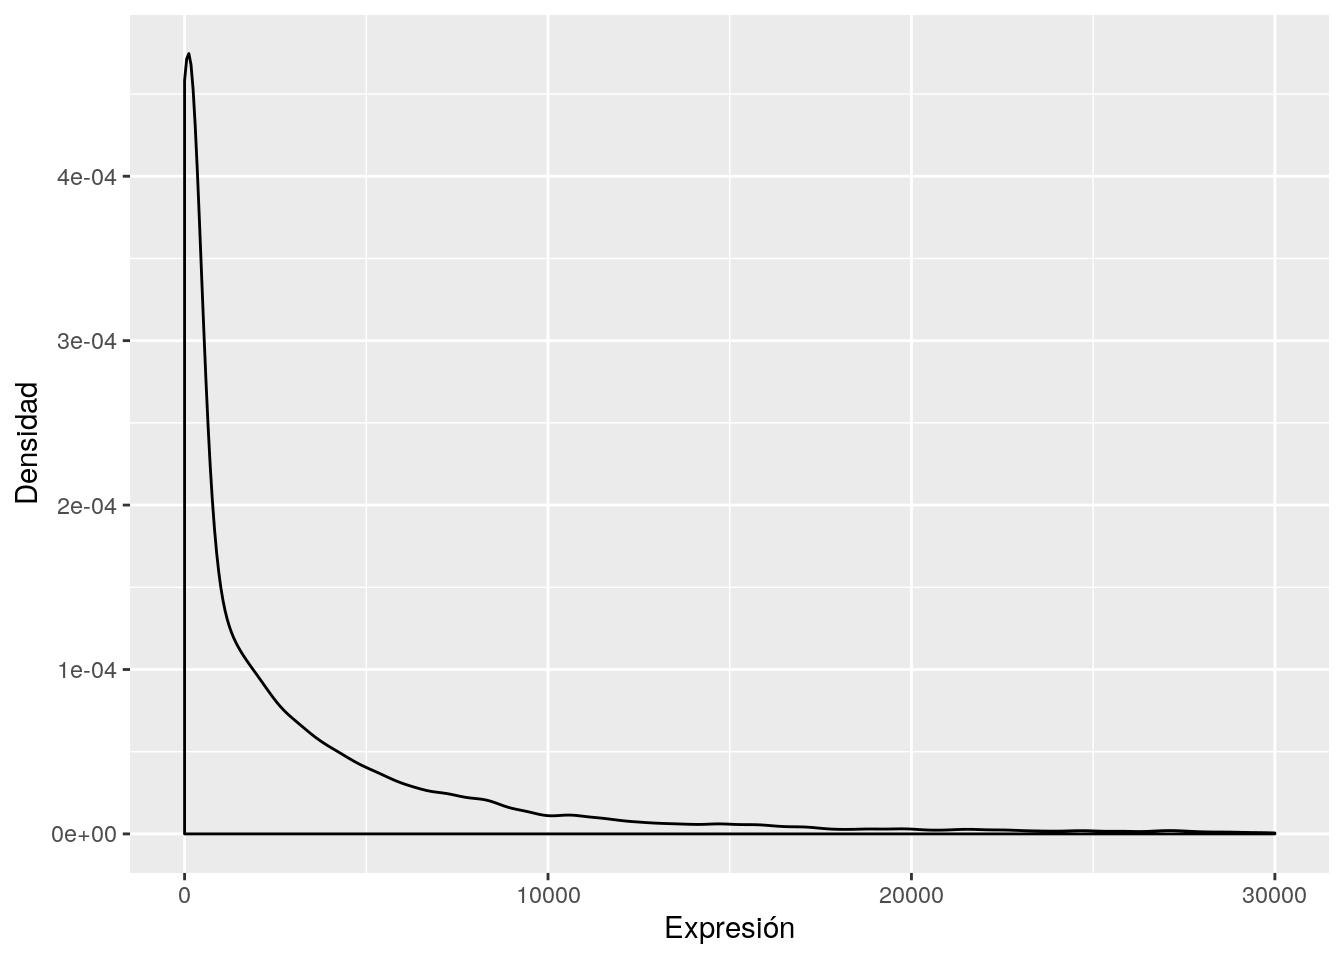
\includegraphics[width=0.7\linewidth]{02_fuentes_datos_files/figure-latex/rnaDens-1} 

}

\caption{Densidad de los valores de expresión de los genes de un sujeto, para datos obtenidos mediante Secuenciación de ARN.}\label{fig:rnaDens}
\end{figure}
\par

La era de la transcriptómica tuvo su máximo desarrollo con la evolución de las tecnologías de secuenciación de alto rendimiento. La exploración de todo el transcriptoma simultáneamente y a profundidades sin precedentes ha sido posible a partir de estas tecnologías. Esta terminología se refiere a alto rendimiento, en el sentido del paralelismo en la secuenciación, lo que permite investigar millones de fragmentos de ADN en una sola ejecución. Su rápida expansión se justifica por su versatilidad, que ha permitido el estudio de experimentos complejos a escalas hasta ahora inalcanzables e incluso en organismos nunca antes estudiados.

\par

Con el desarrollo de este tipo de tecnología no solo se logró obtener información de expresión a nivel de \textbf{genes}, sino que al tener las cadenas de nucleótidos, es posible extraer información de expresión a niveles biológicos menores que genes, como ser \textbf{transcriptos}, \textbf{exones}, \textbf{isoformas}, etc.

\hypertarget{sec:repos}{%
\section{Repositorios de datos de expresión}\label{sec:repos}}

Para los diversos análisis realizados en la presente tesis, nos centramos principalmente en datos de cáncer de mama. Sin embargo, también se utilizaron repositorios con datos de cáncer de próstata. Un detalle de las bases de datos de libre acceso utilizadas se puede observar en la Tabla \ref{tab:databases}. A lo largo de este trabajo se utilizaron un total de 25 matrices de expresión de cáncer de mama y cuatro de cáncer de próstata, provenientes de microarreglos de ADN.

\par

Adicionalmente se utilizaron datos de cáncer de mama provenientes del proyecto ``el atlas del genoma del cáncer'' (TCGA; del inglés \emph{The Cancer Genome Atlas}). El proyecto TCGA provee, para una misma muestra, niveles de expresión provenientes de diversas fuentes ómicas, de este proyecto se utilizaron matrices de expresión de microarreglos de ADN, de proteínas medidas mediante iTRAQ, y de genes medidos mediante secuenciación de ARN. Vale la pena aclarar que no necesariamente para toda muestra perteneciente al TCGA se cuenta con datos provenientes de las tres tecnologías, en este sentido, se cuenta con 97 sujetos con muestras de las tres tecnologías.
\begin{longtable}[]{@{}lccccc@{}}
\caption{Bases de datos utilizadas en la presente tesis.\label{tab:databases}
Nombre de la base de datos; tipo de cáncer que presentan los sujetos; tecnología de obtención de información biológica utilizada; cantidad de genes presentes; cantidad de sujetos; referencias a la fuente de datos.}\tabularnewline
\toprule
Nombre & Cáncer & Tecnología & \#Genes & \#Muestras & Referencias\tabularnewline
\midrule
\endfirsthead
\toprule
Nombre & Cáncer & Tecnología & \#Genes & \#Muestras & Referencias\tabularnewline
\midrule
\endhead
Camcap & Próstata & Microarreglos & 18.718 & 199 & (Ross-Adams et al., 2015)\tabularnewline
Grasso & & & 17.289 & 122 & (Grasso et al., 2012)\tabularnewline
Taylor & & & 17.950 & 179 & (Taylor et al., 2010)\tabularnewline
Varambally & & & 17.043 & 19 & (Varambally et al., 2005)\tabularnewline
Mainz & Mama & & 13.091 & 200 & (Schmidt et al., 2008)\tabularnewline
Nki & & & 13.120 & 337 & (Van't Veer et al., 2002)\tabularnewline
Transbig & & & 13.091 & 198 & (Chin et al., 2006)\tabularnewline
Unt & & & 18.528 & 133 & (Sotiriou et al., 2006)\tabularnewline
Upp & & & 18.528 & 251 & (Miller et al., 2005)\tabularnewline
Vdx & & & 13.091 & 344 & (Minn et al., 2007)\tabularnewline
& & & & & (Wang et al., 2005)\tabularnewline
Cal & & & 13.091 & 118 & (Chin et al., 2006)\tabularnewline
Dfhcc & & & 20.365 & 115 & (Li et al., 2010)\tabularnewline
Dfhcc2 & & & 20.365 & 84 & (Silver et al., 2010)\tabularnewline
Dfhcc3 & & & 20.365 & 40 & (Richardson et al., 2006)\tabularnewline
Duke2 & & & 20.389 & 160 & (Bonnefoi et al., 2007)\tabularnewline
Emc2 & & & 20.365 & 204 & (Bos et al., 2009)\tabularnewline
Eortc10994 & & & 13.091 & 49 & (Farmer et al., 2005)\tabularnewline
Expo & & & 20.365 & 353 & (Bittner, 2005)\tabularnewline
Hlp & & & 19.985 & 53 & (Natrajan et al., 2010)\tabularnewline
Irb & & & 20.365 & 129 & (Lu et al., 2008)\tabularnewline
Lund2 & & & 12.288 & 105 & (Saal et al., 2007)\tabularnewline
Maqc2 & & & 13.091 & 230 & (Shi et al., 2006)\tabularnewline
Mccc & & & 19.949 & 75 & (Waddell et al., 2010)\tabularnewline
Mda4 & & & 13.091 & 129 & (Liedtke et al., 2008)\tabularnewline
& & & & & (Hess et al., 2006)\tabularnewline
Msk & & & 13.091 & 99 & (Minn et al., 2005)\tabularnewline
Nccs & & & 13.091 & 183 & (Yu et al., 2008)\tabularnewline
Pnc & & & 20.365 & 92 & (Dedeurwaerder et al., 2011)\tabularnewline
Stk & & & 18.528 & 159 & (Pawitan et al., 2005)\tabularnewline
Unc4 & & & 17.779 & 305 & (Prat et al., 2010)\tabularnewline
TCGA & & & 16.207 & 547 & (Weinstein et al., 2013)\tabularnewline
TCGA & & ARN & 19.948 & 547 & (Weinstein et al., 2013)\tabularnewline
TCGA & & iTRAQ & 10.625 & 105 & (Weinstein et al., 2013)\tabularnewline
\bottomrule
\end{longtable}
\hypertarget{condiciones-experimentales}{%
\section{Condiciones experimentales}\label{condiciones-experimentales}}

Como se mencionó en la Sección \ref{sec:af}, para llevar a cabo el AF, es necesario contar con dos condiciones de interés a contrastar. Es decir, dos condiciones para las cuales encontrar aquellos mecanismos biológicos que las diferencian.

\hypertarget{sec:bcSubt}{%
\subsection{Cáncer de mama}\label{sec:bcSubt}}

Para cáncer de mama, Perou et al. (Parker et al., 2009) desarrolló un clasificador - PAM50 - que, a partir de datos de microarreglos de ADN, asigna a cada sujeto en uno de 5 subtipos: Luminal A, Luminal B, Her2, Basal ó Normal. Dicha clasificación se basa en los niveles de expresión detectados, para cada sujeto, en 50 genes específicos (Parker et al., 2009). Contrastar de a pares estos grupos resulta de un alto interés biológico ya que se sabe que cada grupo es diferente al resto en aspectos como tiempo de sobrevida, reacción a distintas drogas, entre otros. Y por ende, los términos biológicos característicos de cada grupo PAM50 son los que determinan su comportamiento. Para cada sujeto se obtuvo su clasificación PAM50 mediante el paquete de R \texttt{genefu} (Gendoo et al., 2015).

\hypertarget{cancer-de-prostata}{%
\subsection{Cáncer de próstata}\label{cancer-de-prostata}}

En el caso del cáncer de próstata, ya que contamos con solo cuatro bases de datos, y una de ellas con solo 19 sujetos, no se contrastaron subtipos de la enfermedad. Para este tipo de cáncer se contrastaron aquellas muestras provenientes de tejido tumoral contra provenientes de tejido normal. De aquí se desea detectar aquellos términos biológicos que caractericen el desarrollo de un tumor maligno en comparación a uno benigno.

\hypertarget{comentarios-finales-1}{%
\section{Comentarios finales}\label{comentarios-finales-1}}

Gracias al rápido avance de las tecnologías de obtención de expresión biológica disminuyeron notablemente sus costos, y por ende, el aumento de proyectos internacionales con mayor número de muestras y nivel de detalle. La disponibilidad libre de estas fuentes de información biológica crearon oportunidades sin precedentes para estudiar enfermedades humanas. Habiendo grandes cantidades de bases de datos biológicas de diversas poblaciones, como de distintas tecnologías ómicas, la integración de información resulta en una herramienta clave para el estudio de enfermedades (Cleveland, 2001). Sin embargo, este tipo de estudios se viene realizando a nivel de poblaciones individuales.

Resulta fundamental llevar este tipo de análisis a la comparación de diversas poblaciones. Integrando información funcional de diversos repositorios como de distintas fuentes moleculares es posible llegar a una caracterización de cada grupo de interés. Atacando aspectos funcionales activos por uno u otro grupo bajo estudio se logra el desarrollo de terapias personalizadas. Es por ello que resulta fundamental poder realizar una comparación y caracterización de múltiples fuentes de datos y poblaciones a nivel funcional.

\hypertarget{cap:ifa}{%
\chapter{Análisis Funcional Integrador}\label{cap:ifa}}

\hypertarget{motivacion}{%
\section{Motivación}\label{motivacion}}

\par

La complejidad y heterogeneidad de ciertas enfermedades, como el cancer, demuestran que el análisis de los genes Diferencialmente Expresados (DE) no resulta suficiente para descrifrar el fenómeno biológico subyacente (Reis-Filho \& Pusztai, 2011). Por el contrario, resulta solo el punto de partida de un proceso de exploración en el que se buscan patrones utilizando diversas fuentes de información (Goeman \& Bühlmann, 2007), un proceso conocido como Análisis Funcional (AF), el cuál fue descripto en el Capítulo \protect\hyperlink{cap:af}{1}. Existen principalmente dos enfoques para llevar a cabo el AF: el Análisis de Sobre-Representación (ASR), y la Puntuación Funcional de Clase (PFC) (Manoli et al., 2006; Pavlidis, Qin, Arango, Mann, \& Sibille, 2004). Una de las principales críticas al ASR es que requiere de una lista de genes candidatos definida por el usuario, generalmente estableciendo un umbral de corte de los genes DE (Goeman \& Bühlmann, 2007; Khatri, Sirota, \& Butte, 2012; Manoli et al., 2006; Pavlidis et al., 2004; Tian et al., 2005). Es por ello que los métodos de PFC emergen como una alternativa que supera esa limitación utilizando no solo todos los genes presentes en el experimento, sino que también sus niveles de expresión, donde los genes son ponderados de acuerdo a alguna métrica relacionada con el fenotipo analizado (Subramanian et al., 2005).

\par

Se han propuesto varios algoritmos tanto de ASR como de PFC (Khatri et al., 2012), cada uno con supuestos y parámetros de entrada diferentes, los cuales pueden conducir a resultados muy diferentes. Adicionalmente, algunas ontologías, como Gene Ontology (Ashburner et al., 2000), organizan sus conjuntos de genes en alguna estructura particular que permite considerar estrategias de penalización adicionales para el AF. Por lo tanto, la selección del algoritmo apropiado y sus parámetros no resulta una decisión trivial para el investigador, y es una problemática que no ha sido abordada analíticamente. Por otra parte, no está claro qué se obtiene con cada método desde un punto de vista de recuperación de la información, si los resultados son independientes del método y sus parámetros o si los métodos son complementarios o igualmente útiles.

\par

Manoli et al. (Manoli et al., 2006) realizó una comparación de ambos enfoques: ASR y PFC. Sin embargo, dicha comparación fue teniendo en cuenta solo 20 conjuntos de genes enriquecidos de los 227 que evaluó, y solo tres bases de datos con 160 sujetos en total. Por otra parte, Pavlidis et al. (Pavlidis et al., 2004) también comparó ambos enfoques, en ese trabajo se utilizaron 41 muestras apareadas de cerebro, y consideró sólo 10 de los conjuntos de genes de los 965 que analizó. Sin embargo, tanto Manoli como Pavlidis obtuvieron resultados inesperados de PFC, ya que evaluaron sólo un algoritmo y con una única parametrización posible, la cual no es comúnmente recomendada por la literatura para el algoritmo utilizado. Es por ello que, para lograr diseñar un mejor enfoque del AF, resulta fundamental un análisis exhaustivo que tenga en cuenta una variedad de algoritmos, de parametrizaciones, una gran cantidad de conjuntos de genes, así como más bases de datos y sujetos.

\hypertarget{validacion-de-resultados}{%
\section{Validación de resultados}\label{validacion-de-resultados}}

\par

Uno de los principales inconvenientes en la comparación de métodos de AF es la falta de \emph{gold standards} o de un conjunto de datos de referencia. Como lo establece Khatri y colaboradores (Khatri et al., 2012); para esta situación, el uso de conjuntos de datos biológicos reales es preferible a datos simulados, ya que estos últimos carecen de factores biológicos importantes (Khatri et al., 2012). Para superar este problema, en el presente trabajo proponemos el uso de varios experimentos para evaluar los mismos (y muy contrastantes) fenotipos de cáncer, asumiendo que deberían exhibir perfiles funcionales similares a través de los experimentos. Nuestra hipótesis es que en un meta-análisis que contrasta dos fenotipos con diferencias conocidas, los patrones de enriquecimiento funcional deben encontrarse en consenso compartidos entre todos los conjuntos de datos, independientemente del método utilizado. Por otra parte, las diferencias entre cohortes podrían considerarse como particularidades biológicas que pueden explorarse más a fondo. Por ejemplo, aunque se encontró poca o ninguna superposición de genes entre varias firmas moleculares en diferentes cohortes de pacientes con el mismo fenotipo (Ein-Dor, Zuk, \& Domany, 2006), se han reportado funcionalidades comunes en términos de funciones biológicas (Reis-Filho \& Pusztai, 2011). Por lo tanto, los resultados del AF deberían ser similares, mostrando un alto consenso entre los conjuntos de datos a pesar de los genes expresados diferencialmente en cada caso.

Adicionalmente, para determinar si los resultados de enriquecimiento están realmente relacionados con la condición bajo estudio, se requerirá una validación manual de la literatura, lo cual suele ser una tarea tediosa para el investigador, por lo que a modo de validación automática, resulta de extrema utilidad la Base de Datos de Toxicogenómica Comparada (BDTC). Utilizando la BDTC (Davis et al., 2014), es posible consultar para un término biológico dado, si el mismo está relacionado o no con una determinada enfermedad. La BDTC se utilizó para, programáticamente, consultar y verificar si los términos enriquecidos por cada método están relacionados o no con la enfermedad bajo estudio: ``cáncer de mama''.

\hypertarget{datos-de-entrada}{%
\section{Datos de entrada}\label{datos-de-entrada}}

\hypertarget{matrices-de-expresion}{%
\subsection{Matrices de expresión}\label{matrices-de-expresion}}

Para el presente trabajo, se analizaron seis bases de datos de cáncer de mama, seleccionadas debido a su fácil acceso ya que se encuentran presentes en el repositorio R \textbf{Bioconductor}. Estas bases de datos fueron medidas mediante la tecnología de microarreglos de ADN y son: Mainz, Nki, Transbig, Unt, Upp y Vdx; ver la Tabla \ref{tab:databases}. Para cada una de las bases de datos, se obtuvo el subtipo intrínseco de cáncer de mama de cada sujeto mediante el método PAM50 (Parker et al., 2009) utilizando la librería de R \texttt{genefu} (Gendoo et al., 2015) y siendo procesados como sugiere Sørlie et al. (Sørlie et al., 2010). Se mantuvieron únicamente aquellos sujetos clasificados como tipo Basal o Luminal A, obteniendo un total de 741 sujetos, ya que es sabido que ambos subtipos son muy contrastantes. Al comparar sobrevida de sujetos de ambos subtipos, Luminal A suele presentar un mejor pronóstico que Basal (Dai et al., 2015; Ein-Dor, Kela, Getz, Givol, \& Domany, 2005; Parker et al., 2009). Por ende, se espera identificar muchos genes que se comporten contrariamente, es decir, desregulados entre ambas condiciones, y que impacten en varios términos (enriquecidos) que se detecten en común a través de las bases de datos. Para cada una de las seis matrices de expresión, se mantuvieron solo aquellos genes que contaban con identificador de genes \emph{Entrez id} válido, y valores de expresión detectados en al menos el 50\% de las muestras de cada subtipo.

\hypertarget{conjuntos-de-genes}{%
\subsection{Conjuntos de genes}\label{conjuntos-de-genes}}

Como Conjuntos de Genes (CG) se utilizaron las tres categorías de GO. Para descargar los CG se utilizó la versión \emph{v3.0.0} del paquete R \texttt{org.Hs.eg.db} (Carlson, Falcon, Pages, \& Li, 2013), obteniendo un total de 19.693 CG.

\hypertarget{sec:algosComparados}{%
\section{Algoritmos y parámetros comparados}\label{sec:algosComparados}}

Para determinar si un CG se encontraba enriquecido por un método dado, se utilizaron los criterios por defecto o recomendados de cada método.

\hypertarget{analisis-de-sobre-representacion}{%
\subsection{Análisis de Sobre-Representación}\label{analisis-de-sobre-representacion}}

Dentro de los algoritmos de ASR, una de las herramientas más utilizadas es la plataforma web DAVID (Huang, Sherman, \& Lempicki, 2009) -del inglés \emph{Database for Annotation, Visualization and Integrated Discovery}-. La lista de genes DE de cada base de datos fue enviada a la plataforma Web DAVID (en adelante llamado \textbf{WD}) a través del paquete R \texttt{RDAVIDWebService} (Fresno \& Fernández, 2013). Uno de los principales inconvenientes de la plataforma DAVID es que no permite evaluar CG provistos por el usuario, y al momento de realizar este análisis, la versión estable (\emph{v6.7}) contaba con una base de conocimiento actualizada por última vez en el año 2010. Para superar este inconveniente, desarrollamos \textbf{RD}, una versión en lenguaje R del algoritmo de DAVID, que nos permite analizar cualquier CG de interés. Además, a diferencia de DAVID y RDAVIDWebService, RD no requiere de comunicación a través de internet. El tercer algoritmo de ASR evaluado es \textbf{GOstats} (Falcon \& Gentleman, 2007), que fue diseñado específicamente para realizar análisis de enriquecimiento de GO. GOstats penaliza el enriquecimiento de los CG (penalización \emph{elim}) teniendo en cuenta la estructura de grafos de GO. Finalmente, también se evaluó el método \textbf{dEnricher} (Fang \& Gough, 2014). Este último método posee una representación interna de GO, y ofrece otro método de penalización adicional al provisto por GOstats (penalización \emph{lea}). Además dEnricher permite seleccionar el test estadístico a utilizar: \emph{Hipergeométrico}, \emph{Binomial} ó \emph{Fisher}.

\par

Como se mencionó en la Sección \ref{sec:af}, los métodos de ASR requieren, además de los CG y la lista de genes candidatos, la lista de genes de referencia (BR; del inglés \emph{Background Reference}). Utilizar diferentes listas de referencia pueden dar lugar a resultados diferentes del método de ASR (Fresno et al., 2012; Rivals, Personnaz, Taing, \& Potier, 2007). Por ello, para cada opción de ASR propuesta, a excepción de dEnricher que no lo permite, se evaluaron listas de referencia propuestas por Fresno et al. (Fresno et al., 2012). Las listas de referencia evaluadas fueron: el genoma completo (BRI) y aquellos genes detectados en el experimento (BRIII).

\par

Para cada base de datos, como lista de genes candidatos, se utilizaron los genes DE del experimento. Para obtener los genes DE de cada experimento se utilizó la función \texttt{treat} (McCarthy \& Smyth, 2009) del paquete R \texttt{limma} (Berkeley, 2004), esta función tiene en cuenta aquellos genes que presentan un valor absoluto de Fold-Change mayor a un valor de corte llamado \emph{treatLfc}. Los genes DE fueron aquellos que obtuvieron un p-valor ajustado por FDR \(\leq\) 0,01. Para obtener resultados comparables entre los experimentos, para cada base de datos, se seleccionó un valor \emph{treatLfc} que obtuviera una cantidad de genes DE de alrededor el 5\% de la longitud de su BRIII.

\par

En resumen, los métodos y parámetros analizados de ASR, junto con el identificador a utilizar (en negrita), se listan a continuación:
\begin{small}
\[
\begin{matrix}
DAVID\left\{\begin{matrix}
       BRI\;\;\;\;\;\;\;\;\;\;\;\;\;\;\;\;\;\;\;\;\;\;\;\;\;\;\;\;\;\;\;\;\;\;\;\;\;\;\;\;\;\;\;\;\;\;\;\;\;\;\;\;\textbf{WD BRI}
    \\ BRIII\;\;\;\;\;\;\;\;\;\;\;\;\;\;\;\;\;\;\;\;\;\;\;\;\;\;\;\;\;\;\;\;\;\;\;\;\;\;\;\;\;\;\;\;\;\textbf{WD BRIII}
\end{matrix}\right.
\end{matrix}
\]
\[
\begin{matrix}
RD\;\;\;\;\;\;\; \left\{\begin{matrix}
       BRI\;\;\;\;\;\;\;\;\;\;\;\;\;\;\;\;\;\;\;\;\;\;\;\;\;\;\;\;\;\;\;\;\;\;\;\;\;\;\;\;\;\;\;\;\;\;\;\;\;\;\;\;\;\textbf{RD BRI}
    \\ BRIII\;\;\;\;\;\;\;\;\;\;\;\;\;\;\;\;\;\;\;\;\;\;\;\;\;\;\;\;\;\;\;\;\;\;\;\;\;\;\;\;\;\;\;\;\;\;\textbf{RD BRIII}
\end{matrix}\right.
\end{matrix}
\]
\[
\begin{matrix}
GOstats\left\{\begin{matrix}
       BRI\;\;\;\;\;\;\;\;\;\;\;\;\;\;\;\;\;\;\;\;\;\;\;\;\;\;\;\;\;\;\;\;\;\;\;\;\;\;\;\;\;\;\;\;\;\textbf{GOstats BRI}
    \\ BRIII\;\;\;\;\;\;\;\;\;\;\;\;\;\;\;\;\;\;\;\;\;\;\;\;\;\;\;\;\;\;\;\;\;\;\;\;\;\;\textbf{GOstats BRIII}
\end{matrix}\right.
\end{matrix}
\]
\[
\begin{matrix}
dEnricher \left\{\begin{matrix}
       \begin{matrix}Hipergeo-\\ métrico\end{matrix} \left\{\begin{matrix}
           sin\;penalizar\;\;\;\;\;\;\;\;\;\textbf{dE\_H\_none}
        \\ lea\;\;\;\;\;\;\;\;\;\;\;\;\;\;\;\;\;\;\;\;\;\;\;\;\;\;\;\;\textbf{dE\_H\_lea}
        \\ elim\;\;\;\;\;\;\;\;\;\;\;\;\;\;\;\;\;\;\;\;\;\;\;\;\textbf{dE\_H\_elim}
    \end{matrix}\right.
    \\ Binomial\;\;\;\; \left\{\begin{matrix}
           sin\;penalizar\;\;\;\;\;\;\;\;\;\;\textbf{dE\_b\_none}
        \\ lea\;\;\;\;\;\;\;\;\;\;\;\;\;\;\;\;\;\;\;\;\;\;\;\;\;\;\;\;\;\textbf{dE\_b\_lea}
        \\ elim\;\;\;\;\;\;\;\;\;\;\;\;\;\;\;\;\;\;\;\;\;\;\;\;\textbf{dE\_b\_elim}
    \end{matrix}\right.
    \\ Fisher\;\;\;\;\;\;\;\;\left\{\begin{matrix}
           sin\;penalizar\;\;\;\;\;\;\;\;\;\textbf{dE\_F\_none}
        \\ lea\;\;\;\;\;\;\;\;\;\;\;\;\;\;\;\;\;\;\;\;\;\;\;\;\;\;\;\;\textbf{dE\_F\_lea}
        \\ elim\;\;\;\;\;\;\;\;\;\;\;\;\;\;\;\;\;\;\;\;\;\;\;\textbf{dE\_F\_elim}
    \end{matrix}\right.
\end{matrix}\right.
\end{matrix}
\]
\end{small}
\hypertarget{puntuacion-funcional-de-clase}{%
\subsection{Puntuación Funcional de Clase}\label{puntuacion-funcional-de-clase}}

El método \emph{Gene Set Enrichment Analysis} propuesto por Subramanian et al. (Subramanian et al., 2005) fue de los primeros algoritmos de PFC. El método Subramanian (SM; del inglés de \emph{Subramanian Method}) se incluyó entre los analizados, se utilizó su implementación en lenguaje Java (\emph{v2-2.2.1.1}), ya que la implementación R se encuentra deprecada. El SM puede ser alimentado con un vector de genes pre-rankeados (\textbf{SMpr}) obtenidos a través de alguna métrica adecuada, ó con la matriz de expresión de genes. Para esta última alternativa, la significancia del estadístico \emph{Enrichment Score} (ES) se estima a través de una estrategia de permutaciones sobre las etiquetas de los genes (\textbf{SMgp}) o de las condiciones a las que pertenece cada muestra (\textbf{SMpp}), generando rankeos permutados de los genes. Para determinar a cada conjunto de genes un p-valor asociado, el SM calcula los ESs aplicando un estadístico de \emph{Kolmogorov-Smirnov} ponderado (Subramanian et al., 2005). Esta ponderación está determinada por un peso \(w\) que, por defecto, se establece en 1, pero que también puede sustituirse por 0 ó 2. Sin embargo, el efecto del peso \(w\) no queda claro ya que los autores sugieren diferentes parametrizaciones de acuerdo con el tipo de dato de entrada (matriz de expresión ó genes pre-rankeados). En el presente trabajo se evaluaron las combinaciones de las diferentes estrategias de permutación con las diferentes alternativas de pesos \emph{w}. Para el caso de SMpr, ya que debe contarse con un vector de rankeo de los genes, se aplicó la función \texttt{eBayes} de la librería R \texttt{limma}, obteniendo así para cada gen, el estadístico \emph{t} y p-valor asociados. Se analizaron tres métodos de rankeo: \(t\), \(1-p\)-\(valor\), y \(-log(p\)-\(valor)\). Los métodos de PFC suelen filtrar conjuntos de genes previo a realizar el análisis. Este filtrado suele darse dependiendo de la cantidad de genes que componen cada CG. Al evaluar el SM se utilizaron los parámetros de filtrado de CG por defecto, que analiza CG que incluyen entre 15 y 500 genes.

\par

Otra alternativa de PFC evaluada fue la librería R \texttt{mGSZ}, la cual se basa en la función de \emph{Z-score} para el cálculo del ES, y en estimación asintótica del p-valor de cada CG, mediante permutaciones de muestras e (implícitamente) de genes (Mishra, Törönen, Leino, \& Holm, 2014). El método mGSZ como entrada requiere la matriz de expresión, y rankea los genes mediante el estadístico \emph{t} moderado (Berkeley, 2004), obtenido utilizando la función \texttt{eBayes} de la librería R \texttt{limma}. El método mGSZ limita el tamaño de los CG, por defecto, usando un mínimo de 5 genes (sin filtrar por máximo). Adicionalmente, se analizó filtrando CG entre 15 y 500, como en el SM, para obtener una comparación más robusta.

\par

En resumen, los métodos y parámetros analizados de PFC, junto con el identificador a utilizar (en negrita), se listan a continuación:
\begin{small}
\[
\begin{matrix}
\begin{matrix}Subra-\\ manian\end{matrix} \left\{\begin{matrix}
    \begin{matrix}Permutación\\ de\; genes\end{matrix} \left\{\begin{matrix}
           w=0\;\;\;\;\;\;\;\;\;\;\;\;\;\;\;\;\;\;\;\;\;\;\;\;\;\;\;\;\;\textbf{SMgp0}
        \\ w=1\;\;\;\;\;\;\;\;\;\;\;\;\;\;\;\;\;\;\;\;\;\;\;\;\;\;\;\;\;\textbf{SMgp1}
        \\ w=2\;\;\;\;\;\;\;\;\;\;\;\;\;\;\;\;\;\;\;\;\;\;\;\;\;\;\;\;\;\textbf{SMgp2}
    \end{matrix}\right.
    \\ \begin{matrix}Permutación\\ de\; condición\end{matrix} \left\{\begin{matrix}
           w=0\;\;\;\;\;\;\;\;\;\;\;\;\;\;\;\;\;\;\;\;\;\;\;\;\;\;\;\;\;\textbf{SMpp0}
        \\ w=1\;\;\;\;\;\;\;\;\;\;\;\;\;\;\;\;\;\;\;\;\;\;\;\;\;\;\;\;\;\textbf{SMpp1}
        \\ w=2\;\;\;\;\;\;\;\;\;\;\;\;\;\;\;\;\;\;\;\;\;\;\;\;\;\;\;\;\;\textbf{SMpp2}
    \end{matrix}\right.
    \\ \begin{matrix}Pre-\\ rank\end{matrix} \left\{\begin{matrix}
           \;\;\;\;\;\;\; t \;\;\;\;\;\;\; \left\{\begin{matrix}
           w=0\;\;\;\;\;\;\;\;\;\;\textbf{SMpr tScore 0}
        \\ w=1\;\;\;\;\;\;\;\;\;\;\textbf{SMpr tScore 1}
        \\ w=2\;\;\;\;\;\;\;\;\;\;\textbf{SMpr tScore 2}
    \end{matrix}\right.
    \\ \begin{matrix}-log\\ p-valor\end{matrix} \left\{\begin{matrix}
           w=0\;\;\;\;\;\;\;\;\;\textbf{SMpr -log(p) 0}
        \\ w=1\;\;\;\;\;\;\;\;\;\textbf{SMpr -log(p) 1}
        \\ w=2\;\;\;\;\;\;\;\;\;\textbf{SMpr -log(p) 2}
    \end{matrix}\right.
    \\ \begin{matrix}1-\\ p-valor\end{matrix} \left\{\begin{matrix}
           w=0\;\;\;\;\;\;\;\;\;\;\;\;\;\;\;\;\textbf{SMpr 1-p 0}
        \\ w=1\;\;\;\;\;\;\;\;\;\;\;\;\;\;\;\;\textbf{SMpr 1-p 1}
        \\ w=2\;\;\;\;\;\;\;\;\;\;\;\;\;\;\;\;\textbf{SMpr 1-p 2}
    \end{matrix}\right.
    \end{matrix}\right.
\end{matrix}\right.
\end{matrix}
\]
\[
\begin{matrix}
mGSZ\;\; \left\{\begin{matrix}
       CG\:filtrado [15,500)\;\;\;\;\;\;\;\;\;\;\;\;\;\;\;\;\;\;\;\textbf{mGSZ[15,500)}
    \\ CG\:filtrado [5,\infty)\;\;\;\;\;\;\;\;\;\;\;\;\;\;\;\;\;\;\;\;\;\;\;\;\;\;\;\mathbf{mGSZ[5,\infty)}
\end{matrix}\right.
\end{matrix}
\]
\end{small}
\hypertarget{resultados}{%
\section{Resultados}\label{resultados}}

\hypertarget{genes-diferencialmente-expresados-por-base-de-datos}{%
\subsection{Genes diferencialmente expresados por base de datos}\label{genes-diferencialmente-expresados-por-base-de-datos}}

\par

El número de genes DE para cada base de datos analizada se presenta en la Tabla \ref{tab:deGenes}. Aunque para cada matriz de expresión se contrastaron los mismos subtipos de cáncer de mama, se observa muy poca superposición entre pares de experimentos. Por ejemplo, los datasets Unt y Nki sólo presentan 383 genes DE en común, siendo que Unt tiene 1.059 genes DE en total (sólo el 36\% se superponen). En general, se encontró que sólo el 12\% (195 genes) de los genes DE en común entre todas los bases de datos (la intersección) se superponen entre la unión (1.678 genes) de los genes DE de todos los datasets evaluados.
\begin{longtable}[]{@{}lcccccc@{}}
\caption{Genes diferencialmente expresados entre bases de datos.\label{tab:deGenes}
Primera columna: Los Nombres de las bases de datos, con el umbral de valor absoluto de Fold-Change entre paréntesis. Diagonal principal: Número de genes Diferencialmente Expresados (DE) para cada base de datos (FDR \(\leq\) 0,01) y porcentaje del total de genes en el experimento entre paréntesis. Triangular superior: Número de genes DE intersectados por cada par de bases de datos. Nótese que la intersección global de genes DE es sólo 195 de una unión total de 1.678 genes DE.}\tabularnewline
\toprule
Nombre & Vdx & Nki & Transbig & Upp & Unt & Mainz\tabularnewline
\midrule
\endfirsthead
\toprule
Nombre & Vdx & Nki & Transbig & Upp & Unt & Mainz\tabularnewline
\midrule
\endhead
Vdx (0,75) & 611 (4,7) & 292 & 465 & 430 & 425 & 412\tabularnewline
Nki (0,2) & & 568 (4,3) & 310 & 374 & 383 & 286\tabularnewline
Transbig (0,6) & & & 628 (4,8) & 448 & 461 & 433\tabularnewline
Upp (0,3) & & & & 932 (5) & 632 & 428\tabularnewline
Unt (0,25) & & & & & 1.059 (5,7) & 437\tabularnewline
Mainz (0,45) & & & & & & 605 (4,6)\tabularnewline
& Intersección: & 195 & & Unión: & 1.678 &\tabularnewline
\bottomrule
\end{longtable}
\hypertarget{analisis-de-estabilidad-de-enriquecimiento}{%
\subsection{Análisis de estabilidad de enriquecimiento}\label{analisis-de-estabilidad-de-enriquecimiento}}

\par

Para evaluar la estabilidad de detección de CG enriquecidos a través de las diversas bases de datos, para cada combinación de método/parámetros, se generó un boxplot con el número de CG enriquecidos. La integración de resultados de diversas bases de datos nos permite proporcionar validación inter-estudios tal y como se indica en el análisis de Edelman et al. (Edelman et al., 2006).

\par

Como se puede observar en los boxplot de la Figura \ref{fig:ifa1}, se aprecia una alta variabilidad tanto entre los métodos como para las diversas parametrizaciones de un mismo método. Teniendo en cuenta solo aquellos datasets que presentaron almenos un término enriquecido, se encontró una mediana de 284 términos enriquecidos. El SM parece ser muy sensible a diferentes parametrizaciones, así como a la forma en que se le proveen los datos, es decir, a través de la matriz de expresión de genes o mediante una lista pre-rankeada. Curiosamente, para SMpr cualquier valor del factor de ponderación \(w\) devolvió casi cero términos enriquecidos. Además, para SMgp y SMpp, la selección de \(w\) podría producir enriquecimientos muy diferentes, que van desde cero términos en SMpp0 para Nki o 59 términos en SMgp2 para Vdx hasta valores extremos como 1.019 en SMpp2 para Nki o 474 términos en SMgp0 para Vdx. En particular, el método SMpp presenta comportamientos muy diferentes dependiendo del valor \(w\). Por ejemplo, no se encontró enriquecimiento para \(w=0\), gran variabilidad resultó con \(w=1\) con un Rango InterCuartil (RIC) de 257,57, y se obtuvieron resultados concordantes con \(w=2\), es decir, pequeña dispersión sobre bases de datos (con un RIC de 83,25). Sin embargo, SMpp2 mostró un número extremo de enriquecimientos para una base de datos (1.019 para Nki) y un número muy bajo para otro (101 para Mainz), resultando en dos valores atípicos. Esto podría plantear un problema cuando se analiza un único dataset. Para el SMgp, el enriquecimiento es bastante estable en todos los datasets, con RICs de 105, 91,25 y 98,5 para SMgp0, SMgp1 y SMgp2, respectivamente, pero se obtuvo un número decreciente de enriquecimientos a medida que \(w\) aumentaba de 0 a 2, lo que arroja una mediana de 611,5, 293 y 121, respectivamente. Para \(w=1\) el número de términos enriquecidos es similar a la mediana general (284 términos enriquecidos) de los diferentes métodos, lo que sugiere que el SMgp1 se podría considerar una configuración más apropiada.
\begin{figure}

{\centering 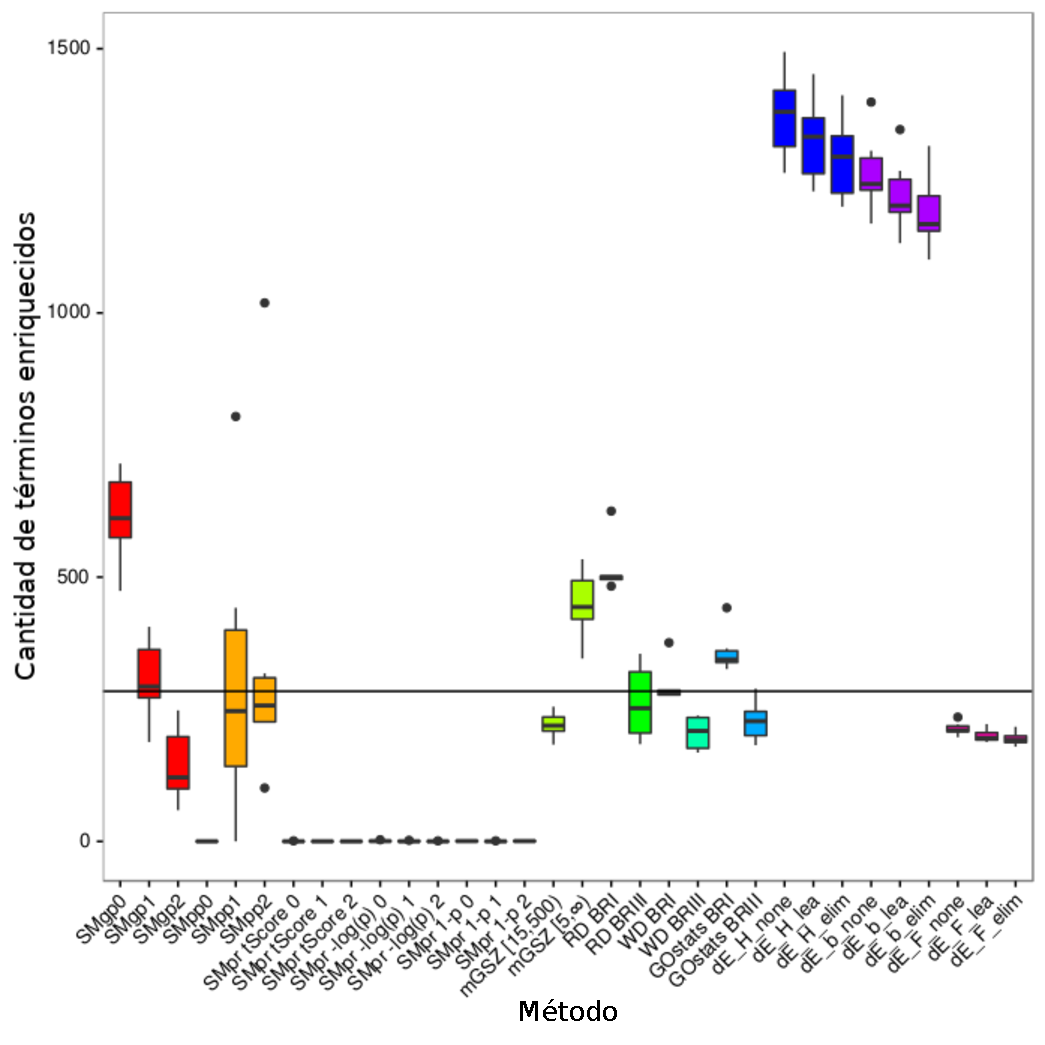
\includegraphics[width=1\linewidth]{images/IFA_FIG1_es} 

}

\caption{Boxplot del número de términos enriquecidos por cada método para las diferentes bases de datos. Las siglas de los métodos se describen en la Sección \ref{sec:algosComparados}. Notar que las alternativas de SMpr enriquecen casi ningún conjunto de genes, mientras que la mediana de términos enriquecidos es de 284 para los métodos restantes (línea negra horizontal). El método SMpp1 obtuvo el número más variable de términos enriquecidos. A excepción de dEnricher con prueba de Fisher, todas las demás combinaciones de método/parámetro de dEnricher devolvieron valores extremos.}\label{fig:ifa1}
\end{figure}


\par

En el caso de mGSZ, los resultados mostraron una estabilidad adecuada entre los datasets (RICs de 26,5 para mGSZ\([15,500)\) y 73 para mGSZ\([5,\infty)\)), produciendo un número muy similar de términos enriquecidos entre las bases de datos. Este método resultó sensible al tamaño de los CG analizados. Cuando el filtro de CG a analizar se estableció entre \([15,500)\), se logró un número bastante conservador de términos enriquecidos, es decir, número menor de CG enriquecidos. Estos resultados fueron más estables en comparación con el valor obtenido con los límites de filtro de CG de \([5,\infty)\). Vale la pena mencionar que los términos enriquecidos obtenidos con filtro \([15,500)\) fueron contenidos en su mayoría (93\% en promedio) por el método con el filtro de CG por defecto. Estos términos enriquecidos adicionales generalmente contenían un menor número de genes, es decir, términos más específicos que pueden ser mucho más útiles para descifrar el fenómeno biológico bajo estudio. Basándonos en este concepto, en adelante, hemos seguido las recomendaciones del autor de mGSZ en cuanto al filtrado de conjuntos de genes de \([5,\infty)\).

\par

A excepción de las diversas parametrizaciones de dEnricher, los resultados de las alternativas de ASR fueron bastante similares entre sí, produciendo enriquecimientos bastante estables en todos los datasets: RICs de 6,25 para RD BRI; 115,75 RD BRIII; 8,75 WD BRI; 58 WD BRIII; 21,75 GOstats BRI; y 45,5 GOstats BRIII. La configuración RD BRIII mostró una mayor variabilidad que su contraparte de WD BRIII, probablemente porque se analizó un mayor número de CG (76\% más CG en promedio). Para cada alternativa de ASR, los enriquecimientos obtenidos con BRIII estaban en general contenidos en los obtenidos utilizando BRI (99\% de los términos en promedio para RD y WD; y 86\% para GOstats) en concordancia con la observación de Fresno et al. (Fresno et al., 2012).

\par

En el caso de dEnricher, las pruebas Hipergeométrica y Binomial arrojaron un número extremo de términos enriquecidos en comparación con la mediana general de los demás métodos, obteniendo más de 1.168 términos enriquecidos, independientemente del algoritmo de penalización aplicado. Por otra parte, la prueba de Fisher arrojó resultados bastante estables, en comparación con los otros métodos de ASR, con valores medios de 210, 195,5 y 191,5 para dE\_F\_none, dE\_F\_lea y dE\_F\_elim, respectivamente; con RICs inferiores a 13,75. Los términos enriquecidos obtenidos con los algoritmos dE\_F\_lea y dE\_F\_elim fueron 100\% contenidos en los obtenidos con dE\_F\_none; más aún, el 86\% de estos términos enriquecidos adicionales encontrados por dE\_F\_none estaban relacionados con el cáncer de mama cuando fueron consultados en la BDTC. Para los siguientes análisis se descartaron las combinaciones de parámetros de dEnricher, excepto dE\_F\_none.

\par

Sólo aquellos métodos y configuraciones que devolvieron un número concordante de términos enriquecidos entre datasets, y alrededor de la mediana general de los métodos (284 términos enriquecidos) fueron considerados para los siguientes análisis, es decir, SMgp1, SMpp2, mGSZ\([5,\infty)\), RD BRI, RD BRIII, WD BRI, WD BRIII, GOstats BRI, GOstats BRIII y dE\_F\_none.

\hypertarget{analisis-de-profundidad-en-gene-ontology}{%
\subsection{Análisis de profundidad en Gene Ontology}\label{analisis-de-profundidad-en-gene-ontology}}

\par

Gene Ontology está organizado en tres grafos acíclicos dirigidos (árboles: ``funciones moleculares'', ``procesos biológicos'' y ``componentes celulares''), donde un nodo hijo representa un término más específico biológicamente que su padre. Para explorar la especificidad biológica sobre la estructura de GO, se calculó el número mínimo de ramas entre el nodo y la raíz (la profundidad) de cada término enriquecido. Luego, se calculó una tabla de frecuencias del número de términos enriquecidos por profundidad (agrupando los resultados para cada base de datos).

\par

El porcentaje de términos enriquecidos agrupados por profundidad para cada método se muestra en la Figura \ref{fig:ifa2}. Todos los métodos tienden a explorar profundidades en su mayoría entre tres y seis. Los métodos mGSZ, dE\_F\_none, SMpp2 y GOstats BRIII enriquecieron el mayor número de términos específicos, es decir, nodos más profundos u hojas, con profundidades \(>\) 6: 13\%, 12,8\%, 10,7\% y 9,8\% del enriquecimiento total, respectivamente. Además, WD y RD proporcionaron mayor enriquecimiento de términos generales, es decir, en profundidades \(<\) 3, nodos más cercanos al nodo raíz de cada árbol de GO: 13,7\% para RD BRI, 11,9\% para WD BRI, 9,7\% para WD BRIII y 8,8\% para RD BRIII. Dentro de los métodos de ASR, proporcionalmente se enriquecen más términos cerca de la raíz cuando se usa BRI que BRIII.

\par

Para cada método de ASR, excepto dEnricher, BRI enriqueció un número mayor de términos que BRIII. Sin embargo, como se mencionó anteriormente, tanto en WD, RD - como en GOstats - la mayoría de los términos enriquecidos por BRIII también fueron enriquecidos por BRI. Como se discutió en Fresno et al., usar BRIII, estadísticamente, tiene más sentido que usar BRI; por lo tanto, su uso se sugiere y se usa de aquí en adelante.
\begin{figure}

{\centering 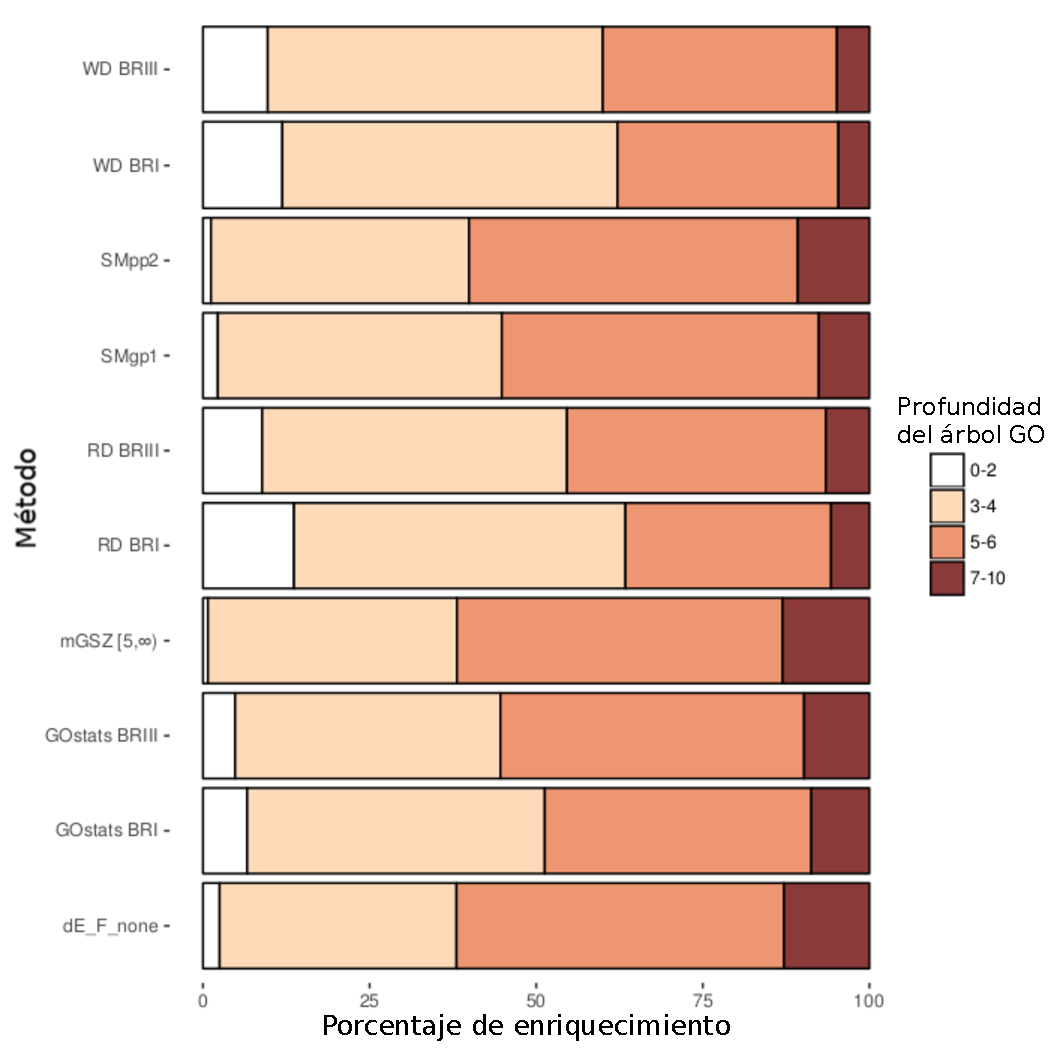
\includegraphics[width=1\linewidth]{images/IFA_FIG2_es} 

}

\caption{Profundidad de enriquecimiento de Gene Ontology (GO) para cada método. Los colores más oscuros representan términos más profundos de la jerarquía del árbol GO. Note que todos los métodos tienden a enriquecer las profundidades en su mayoría entre tres y seis. Los métodos WD y RD enriquecieron los términos más superficiales de la estructura de árbol de GO. Por otro lado, mGSZ, dE\_F\_none, SMpp2 y GOstats BRIII enriquecieron los términos más profundos.}\label{fig:ifa2}
\end{figure}


\hypertarget{sec:consensusSection}{%
\subsection{Análisis de consenso}\label{sec:consensusSection}}

\par

Para evaluar la hipótesis de que los fenotipos comparados deberían presentar perfiles de enriquecimiento similares en todas las bases de datos, se construyó una matriz de enriquecimiento \(E=e_{mdt}\). En esta matriz, cada fila contiene un término GO y cada columna contiene una combinación de método/parámetros por base de datos. Donde cada celda \(e_{mdt}\) de la matriz se definió como sigue:

\[
e_{mdt}=\left\{\begin{matrix}
1 & si\:m\:\mathbf{enriqueció}\:t\:en\:la\:base\:de\:datos\:d \\
0 & si\:m\:\mathbf{no\:enriqueció}\:t\:en\:la\:base\:de\:datos\:d \\
NA & si\:m\:\mathbf{no\:analizó}\:t\:en\:la\:base\:de\:datos\:d
\end{matrix}\right.
\]
donde \(m\) = \{\(1,\ldots,M\)\} combinación de método/parámetros; \(t\) = \{\(1,\ldots,T\)\} un conjunto de genes; \(d\) = \{\(1,\ldots,D\)\} una base de datos.

\par

Aquellos términos que no fueron enriquecidos en ningún conjunto de datos fueron eliminados. Usando la librería R \texttt{vegan}, se aplicó un agrupamiento jerárquico a las filas y columnas de \(E\) a través de la distancia Jaccard y enlace promedio para agrupar automáticamente perfiles de enriquecimiento similares. En la Figura \ref{fig:ifa3} se observa el \emph{heatmap} resultante de la matriz \(E\). El dendrograma superior muestra que los conjuntos de datos analizados tienden a agruparse según el método aplicado, excepto para SMpp2, GOstats y RD, que presentan un conjunto de datos disperso. También puede observarse una diferenciación entre los resultados obtenidos por ASR y PFC, es decir, los métodos de PFC forman un cluster separado, mientras que los métodos de ASR se dividen en dos sub-clusters principales: el de RD/WD y el de GOstats/dE\_F\_none. Como era esperado, puede verse un subconjunto de términos enriquecidos por casi todos los métodos a través de los conjuntos de datos (filas etiquetadas como \textbf{A}). El 64\% de términos enriquecidos en al menos el 80\% de los conjuntos de datos para cada método también fueron enriquecidos por mGSZ en la misma proporción. Esto sugiere que, hasta cierto punto, todos los métodos tienden a proporcionar la misma información. Sin embargo, cada método también proporciona términos exclusivamente enriquecidos (filas etiquetadas como \textbf{E}). La comparación de los métodos de PFC y ASR muestra que RD y WD tienden a enriquecer algunos términos que no se enriquecen por ningún otro método; lo mismo sucede con dE\_F\_none y con mGSZ, lo que sugiere que PFC y ASR se complementan entre sí. Los métodos dE\_F\_none, GOstats y RD, así como mGSZ, analizan más términos que los demás métodos (un número menor de \(e_{mdt}=NA\)). Además, el 63\% de los términos enriquecidos en al menos el 80\% de los conjuntos de datos por los SM también fueron enriquecidos por mGSZ en la misma proporción, mientras que el 47\% de los términos enriquecidos por GOstats, RD y WD fueron enriquecidos por dE\_F\_none, lo que sugiere que mGSZ y dE\_F\_none pueden ser utilizados como métodos de referencia para PFC y ASR, respectivamente.

\par

Dado que todos los experimentos comparan los mismos fenotipos de cáncer de mama, se esperaba encontrar resultados concordantes entre los conjuntos de datos para cada combinación de método/parámetros. Así, el número de términos enriquecidos en casi todos los conjuntos de datos (Frecuencia de Consenso en Enriquecimiento; \(FCE\)), así como los términos que no se enriquecieron en casi todos los conjuntos de datos (Frecuencia de Consenso en No Enriquecimiento; \(FCNE\)), se utilizaron como indicador de la estabilidad del método. Basado en este supuesto, definimos las métricas de comparación listadas en la Tabla \ref{tab:comparisonMetrics}. La concordancia entre los conjuntos de datos para cada método mostró que mGSZ supera con un 45\% de términos enriquecidos concordantes (\(FCE\)), seguido de dE\_F\_none, RD y WD con un 39\%, SMgp1 con un 36\%, SMpp2 con un 30\%, y GOstats con un 29\%. La concordancia entre los términos no enriquecidos (\(FCNE\)) obtuvo 91\% para dE\_F\_none, RD y GOstats, 89\% para WD, 85\% para mGSZ, 83\% para SMgp1, y 82\% para SMpp2. Por lo tanto, todos los métodos parecen tener un alto consenso para los términos no enriquecidos y un bajo consenso para los enriquecidos. Ambos conceptos son importantes a la hora de enfrentarse al AF, ya que no debe perderse ningún término biológicamente significativo, ni debe haber términos enriquecidos incorrectamente. De aquí se desprende que el análisis de PFC utilizando mGSZ demostró ser el método más consensuado, mientras que dE\_F\_none y RD para la contraparte de ASR.
\begin{figure}

{\centering 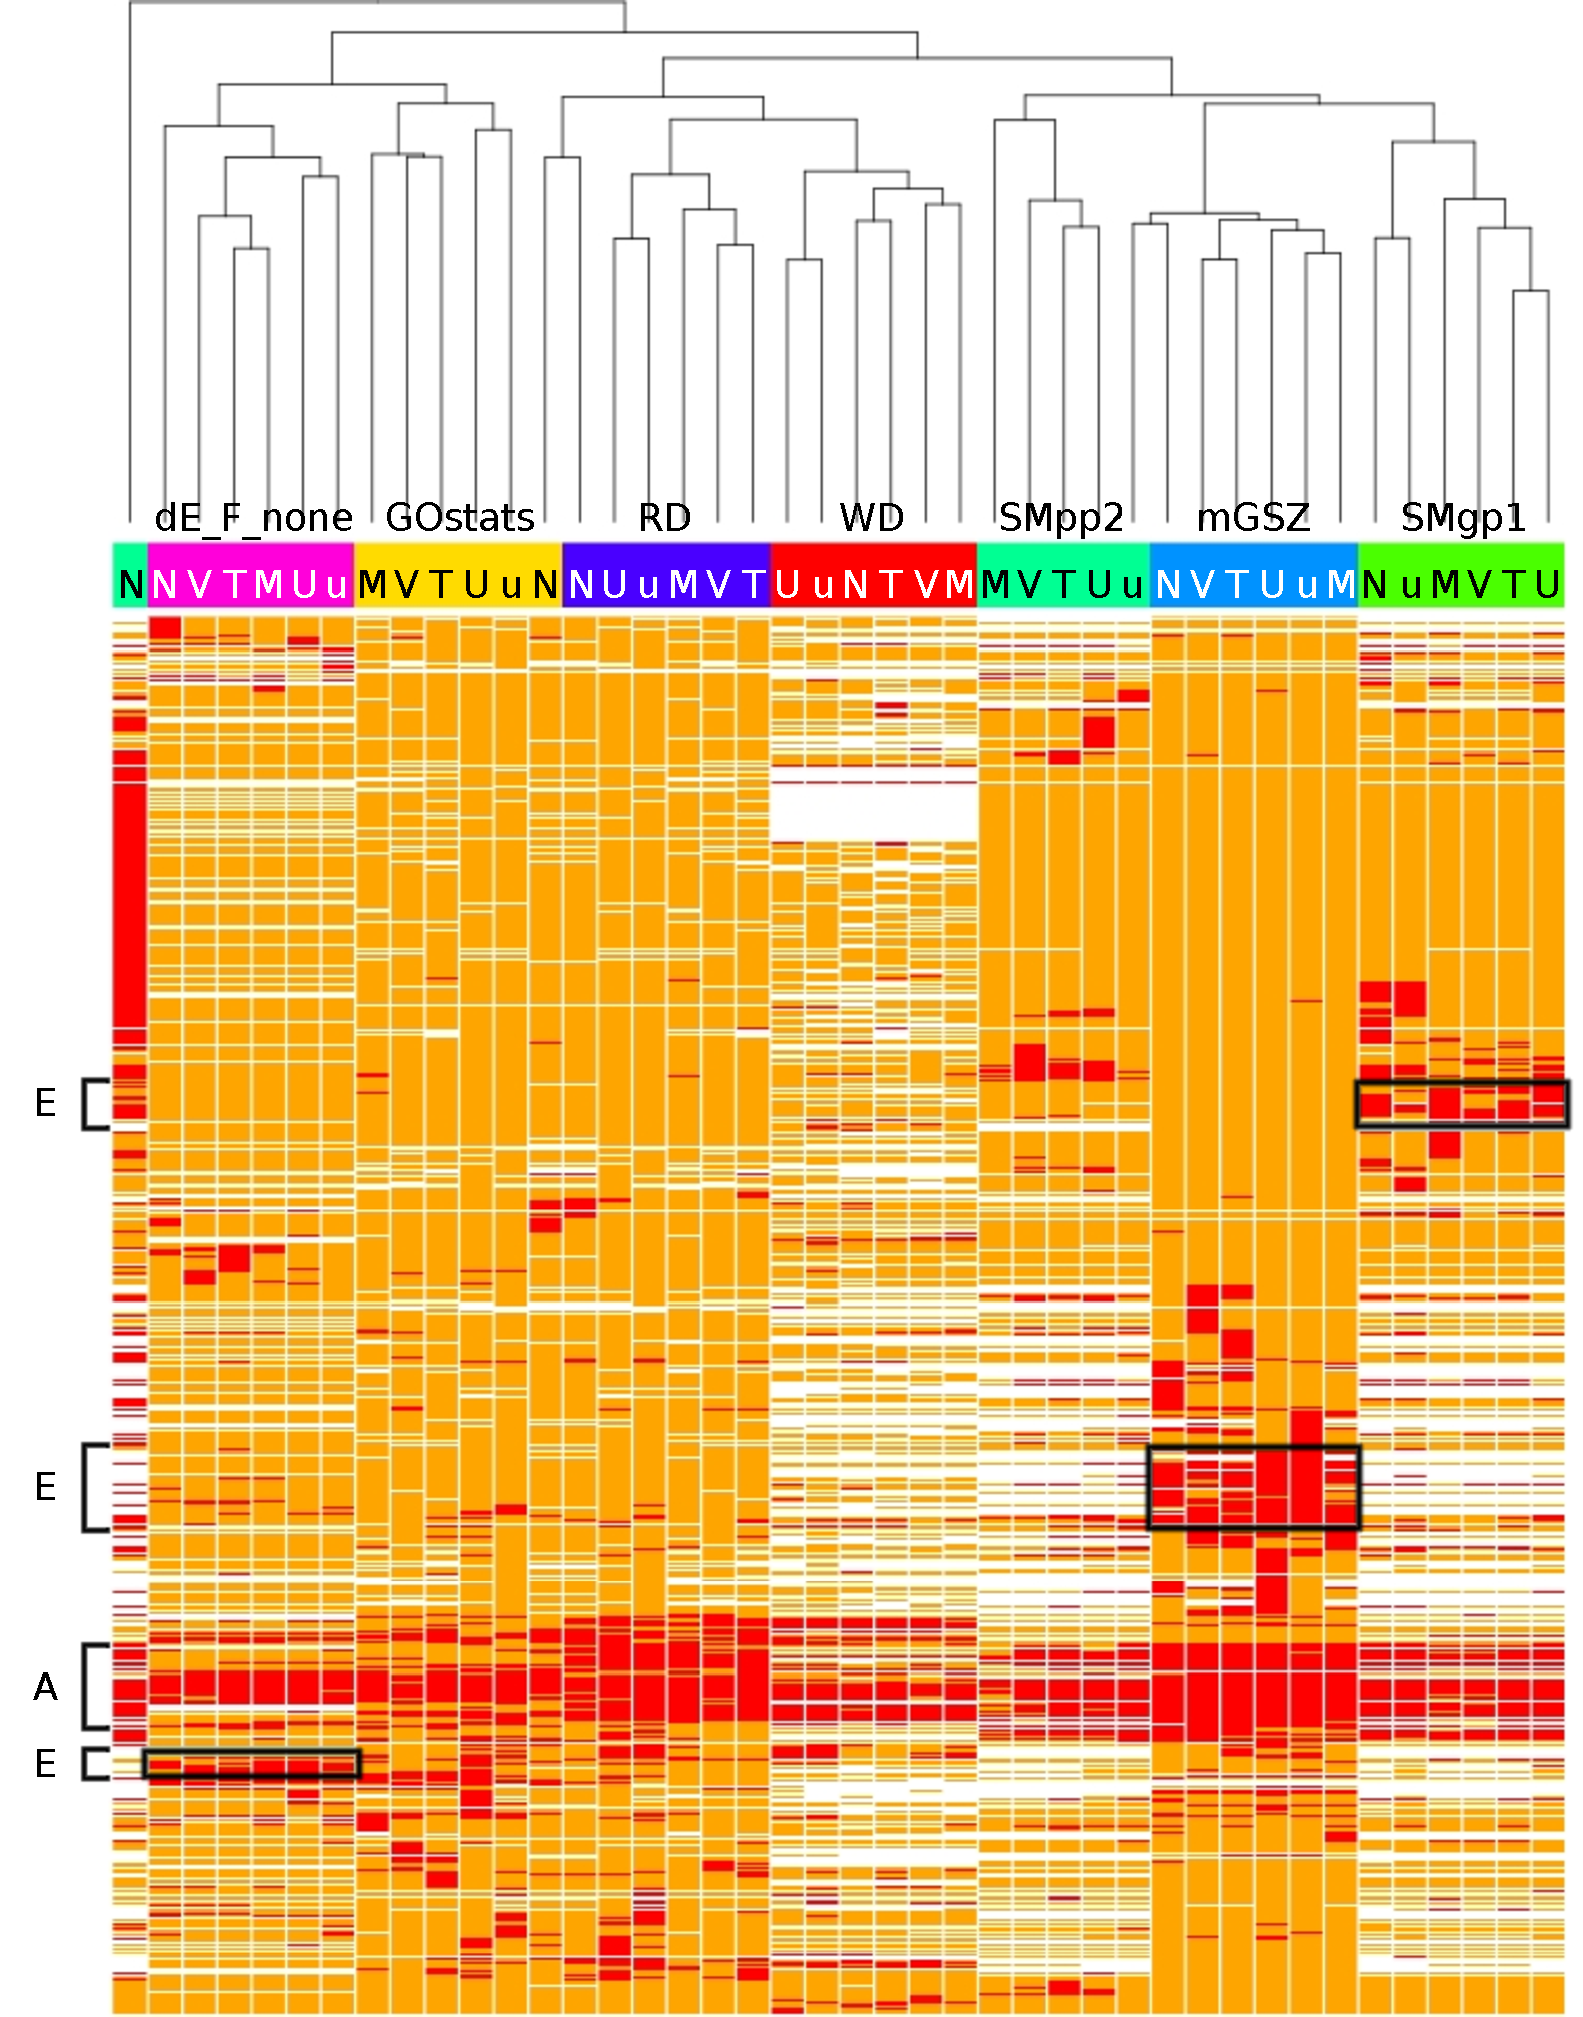
\includegraphics[width=0.9\linewidth]{images/IFA_FIG3} 

}

\caption{Heatmap de enriquecimiento. En columnas, cada combinación de método/parámetros por base de datos; en filas, esos conjuntos de genes (términos) enriquecidos en al menos una base de datos. Notar que los métodos de PFC y ASR se agrupan por separado en el dendrograma. Celdas rojas indican enriquecimiento, naranjas indican que no hay enriquecimiento, y blancas muestran términos que no fueron analizados. Se observan subconjuntos de términos que resultaron enriquecidos por casi todos los métodos analizados (\textbf{A}), y subconjuntos de términos enriquecidos exclusivamente por una sola combinación de método/parámetros (para todas las bases de datos; \textbf{E}). El color de la etiqueta de cada columna representa el algoritmo utilizado, y la letra representa la letra inicial del conjunto de datos: V Vdx; N Nki; T Transbig; U Upp; u Unt; M Mainz.}\label{fig:ifa3}
\end{figure}

\begin{longtable}[]{@{}lc@{}}
\caption{Métricas de comparación.\label{tab:comparisonMetrics}
\(d\) = \{\(1,\ldots,D\)\} base de datos seleccionada; \(t\) = \{\(1,\ldots T\)\} conjunto de genes seleccionado; \(m\): combinación de método/parámetros utilizada; \(t_e=0.8\) y \(t_n=0.2\) umbrales para el enriquecimiento y el no enriquecimiento, respectivamente; \(I\) función indicadora.}\tabularnewline
\toprule
\begin{minipage}[b]{0.44\columnwidth}\raggedright
Nombre\strut
\end{minipage} & \begin{minipage}[b]{0.50\columnwidth}\centering
Definición\strut
\end{minipage}\tabularnewline
\midrule
\endfirsthead
\toprule
\begin{minipage}[b]{0.44\columnwidth}\raggedright
Nombre\strut
\end{minipage} & \begin{minipage}[b]{0.50\columnwidth}\centering
Definición\strut
\end{minipage}\tabularnewline
\midrule
\endhead
\begin{minipage}[t]{0.44\columnwidth}\raggedright
Frecuencia de enriquecimiento inter-método\strut
\end{minipage} & \begin{minipage}[t]{0.50\columnwidth}\centering
\(F_{mt}=\frac{1}{D}\sum_{d=1}^{D}e_{mdt}\)\strut
\end{minipage}\tabularnewline
\begin{minipage}[t]{0.44\columnwidth}\raggedright
Consenso en Enriquecimiento\strut
\end{minipage} & \begin{minipage}[t]{0.50\columnwidth}\centering
\(CE_m=\sum_{t=1}^{T}I(F_{mt} > t_e)\)\strut
\end{minipage}\tabularnewline
\begin{minipage}[t]{0.44\columnwidth}\raggedright
Consenso en No Enriquecimiento\strut
\end{minipage} & \begin{minipage}[t]{0.50\columnwidth}\centering
\(CNE_m=\sum_{t=1}^{T}I(F_{mt} < t_n)\)\strut
\end{minipage}\tabularnewline
\begin{minipage}[t]{0.44\columnwidth}\raggedright
No Consenso\strut
\end{minipage} & \begin{minipage}[t]{0.50\columnwidth}\centering
\(NC_m=\sum_{t=1}^{T}I(t_n \leq F_{mt} \leq t_e)\)\strut
\end{minipage}\tabularnewline
\begin{minipage}[t]{0.44\columnwidth}\raggedright
Frecuencia de \(CE\)\strut
\end{minipage} & \begin{minipage}[t]{0.50\columnwidth}\centering
\(FCE_m=\frac{CE_m}{CE_m+NC_m}\)\strut
\end{minipage}\tabularnewline
\begin{minipage}[t]{0.44\columnwidth}\raggedright
Frecuencia de \(CNE\)\strut
\end{minipage} & \begin{minipage}[t]{0.50\columnwidth}\centering
\(FCNE_m=\frac{CNE_m}{CNE_m+NC_m}\)\strut
\end{minipage}\tabularnewline
\bottomrule
\end{longtable}
\par

Dado que RD fue capaz de analizar más CG que WD, que puede ser utilizado con CG provistos por el usuario, y no depende de una conexión a Internet, se prefirió sobre WD. Por lo tanto, este último fue excluido de los análisis siguientes.

\hypertarget{enriquecimiento-exclusivo-y-relevancia-de-terminos}{%
\subsection{Enriquecimiento exclusivo y relevancia de términos}\label{enriquecimiento-exclusivo-y-relevancia-de-terminos}}

\par

Para determinar si los métodos pueden considerarse complementarios o no desde la perspectiva de la información obtenida, se analizaron los términos exclusivamente enriquecidos (TEE) para cada método, es decir, los términos enriquecidos por el método \(m\) en el 80\% de los datasets, pero en menos del 20\% de los demás \(m' \neq m\), es decir:

\(TEE_m=\{t|F_{mt}>t_e \wedge \forall m' \neq m : F_{m't} < t_n \}\)
donde \(t\) es cualquier conjunto de genes; \(m\) alguna combinación de método/parámetros; \(t_e=0.8\) y \(t_n=0.2\) umbrales para el enriquecimiento y el no enriquecimiento, respectivamente.

\par

Para evaluar la asociación de los términos exclusivamente enriquecidos con el fenotipo bajo estudio, se evaluó la relación de cada término perteneciente a cada \(TEE_m\) utilizando la base de datos dla BDTC (Davis et al., 2014). Utilizando la BDTC, para cada término se pudo determinar su condición patológica en relación con el concepto de ``cáncer de mama''.

\par

Considerando los términos enriquecidos exclusivamente por cada método (\(TEE_m\)), encontramos que mGSZ y dE\_F\_none fueron los que obtuvieron más \(TEE_m\) para PFC y ASR, respectivamente (ver Tabla \ref{tab:eet}). Adicionalmente, mGSZ proporcionó más términos relacionados con el cáncer de mama de acuerdo con la BDTC, así como términos mucho más específicos (profundidad \(>\) 6). En el caso del ASR, dE\_F\_none obtuvo más \(TEE_m\), también relacionados con el cáncer de mama.
\begin{table}[!htbp]
\centering
\caption{Número de términos enriquecidos exclusivos. El número de términos enriquecidos relacionados con el cáncer de mama según la Base de Datos de Toxigenómica Comparativa se presenta entre paréntesis. Notar que mGSZ y dE\_F\_none enriquecen el mayor número de términos para PFC y ASR, respectivamente.}
\begin{tabular}{lccccc}
& \multicolumn{5}{c}{Profundidad en los arboles de GO} \\ \cline{2-6}
Método & 0-2 & 3-4 & 5-6 & 7-10 & Total \\
\hline
SMpp2 & & & 2 (0) & 1 (1) & 3 (1) \\
SMgp1 & 2 (1) & 15 (9) & 7 (4) & & 24 (14) \\
mGSZ & & 26 (13) & 27 (12) & 8 (3) & 61 (28) \\
dE\_F\_none & 1 (1) & 4 (3) & 5 (3) & 3 (1) & 13 (8) \\
RD & 4 (0) & 2 (1) & & & 6 (1) \\
GOstats & & 1 (0) & & & 1 (0) \\
\hline
\end{tabular}
\label{tab:eet}
\end{table}
\hypertarget{sec:ifa}{%
\subsection{Análisis Funcional Integrador}\label{sec:ifa}}

\par

Como resultado de este estudio exhaustivo (Rodriguez, González, Fresno, \& Fernández, 2015; Rodriguez et al., 2016a, 2016b; Rodriguez, Prato, Llera, \& Fernández, 2017), en la Figura \ref{fig:ifa4} se presenta el pipeline del análisis funcional integrador (IFA; del inglés \emph{Integrative Functional Analysis}). El IFA proporciona como una herramienta de software, cuyo código R se encuentra en el repositorio \url{https://github.com/jcrodriguez1989/IFA}. Para utilizar la función principal del IFA, el usuario debe proporcionar la matriz de expresión, y la especificación de los fenotipos de cada sujeto. En caso que no se proporcionen los CG, IFA utilizará los CG de GO más actualizados provistos por la librería R \texttt{org.Hs.eg.db}. La lista de genes DE y su rankeo son calculados por la herramienta IFA mediante un modelo lineal utilizando la librería de R \texttt{limma}, con los cuales se llevan a cabo los análisis mGSZ y de dE\_F\_none. De este modo, IFA proporciona un enfoque sencillo, unificado y global para el AF.
\begin{figure}

{\centering 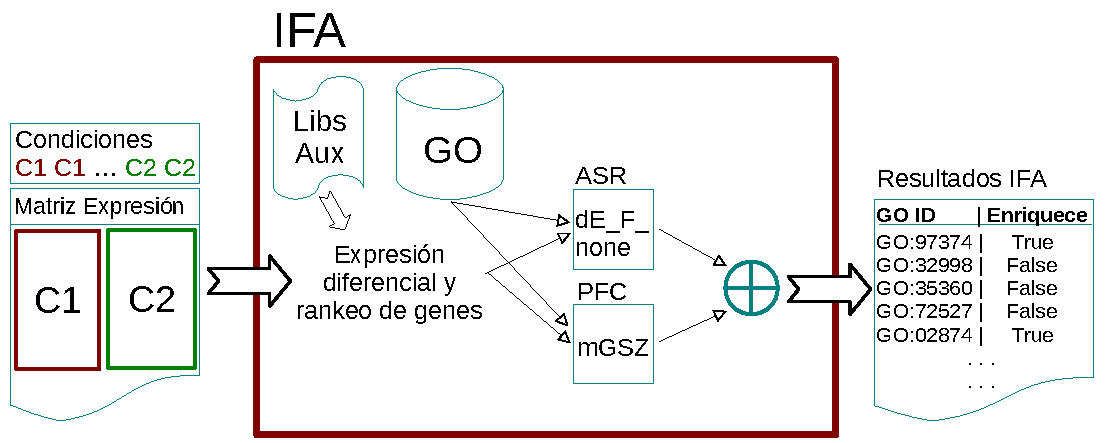
\includegraphics[width=1\linewidth]{images/IFA_FIG4_es} 

}

\caption{Flujo de trabajo del Análisis Funcional Integrador (IFA). El usuario proporciona la matriz de expresión y las correspondientes etiquetas de fenotipo como entrada. El IFA utiliza librerías auxiliares de R para obtener los genes expresados diferencialmente, rankearlos y realizar análisis de PFC y ASR. Finalmente, los resultados de enriquecimiento obtenidos por el IFA integran tanto los resultados del ASR como los de la PFC.}\label{fig:ifa4}
\end{figure}


\hypertarget{ifa-sobre-tcga}{%
\subsection{IFA sobre TCGA}\label{ifa-sobre-tcga}}

\par

Para demostrar la utilidad del pipeline del IFA, se obtuvo el dataset proveniente de microarreglos de ADN de cáncer de mama del reconocido proyecto TCGA. En este dataset, 86 sujetos resultaron clasificados como tipo Basal y 198 como Luminal A. Se utilizó un valor \(treatLfc=1\) de manera de obtener alrededor del 5\% de los genes DE. Los resultados del IFA para este conjunto de datos se utilizaron como caso de prueba y, por lo tanto, se evaluaron y compararon con los conjuntos de datos analizados previamente (Tabla \ref{tab:deGenes}). Como en la Sección \ref{sec:consensusSection}, la matriz de consenso de resultados del IFA se presentó mediante un \emph{heatmap} que se puede observar en la Figura \ref{fig:ifa5}, donde 812 términos resultaron enriquecidos para el conjunto de datos de TCGA. El treinta y tres por ciento de los términos (270) se encontraron enriquecidos también en todos los demás conjuntos de datos (marca \textbf{A} en la Figura \ref{fig:ifa5}), el 43\% (352 términos) se encontraron enriquecidos en más del 80\% de los otros conjuntos de datos, y el 15\% (123 términos) se encontraron enriquecidos exclusivamente en TCGA (marca \textbf{E\(^*\)} en la Figura \ref{fig:ifa5}). En esta matriz de consenso, 445 términos resultaron enriquecidos en al menos el 80\% de todos los conjuntos de datos, de los cuales 232 (52\%) estaban relacionados con el cáncer de mama según la BDTC. En particular, la proporción media de términos exclusivamente enriquecidos presentes en la BDTC en cada conjunto de datos fue del 42\%, con Nki primero con 170 términos exclusivos (84 en la BDTC), y con Mainz último con 58 términos (30 en la BDTC).

\par

Los términos relacionados con la hormona y el receptor de estrógeno, la transición G1/S del ciclo celular mitótico, la replicación del ADN, la organización del huso mitótico, el desenrollado dual del ADN, la actividad de la histona cinasa, la actividad de la helicasa de hibridación, entre otros, se encontraron enriquecidos, en común, en todos los conjuntos de datos (marca \textbf{A} en la Figura \ref{fig:ifa5}), lo que respalda las diferencias de proliferación entre los subtipos de cáncer de mama de tipo Basal y Luminal A. Además, términos como la actividad de la proteína de señalización del receptor tirosina cinasa, la diferenciación de células madre y otros relacionados con la diferenciación celular, sólo se encontraron en los conjuntos de datos de TCGA (marca \textbf{E\(^*\)} en la Figura \ref{fig:ifa5}).
\begin{figure}

{\centering 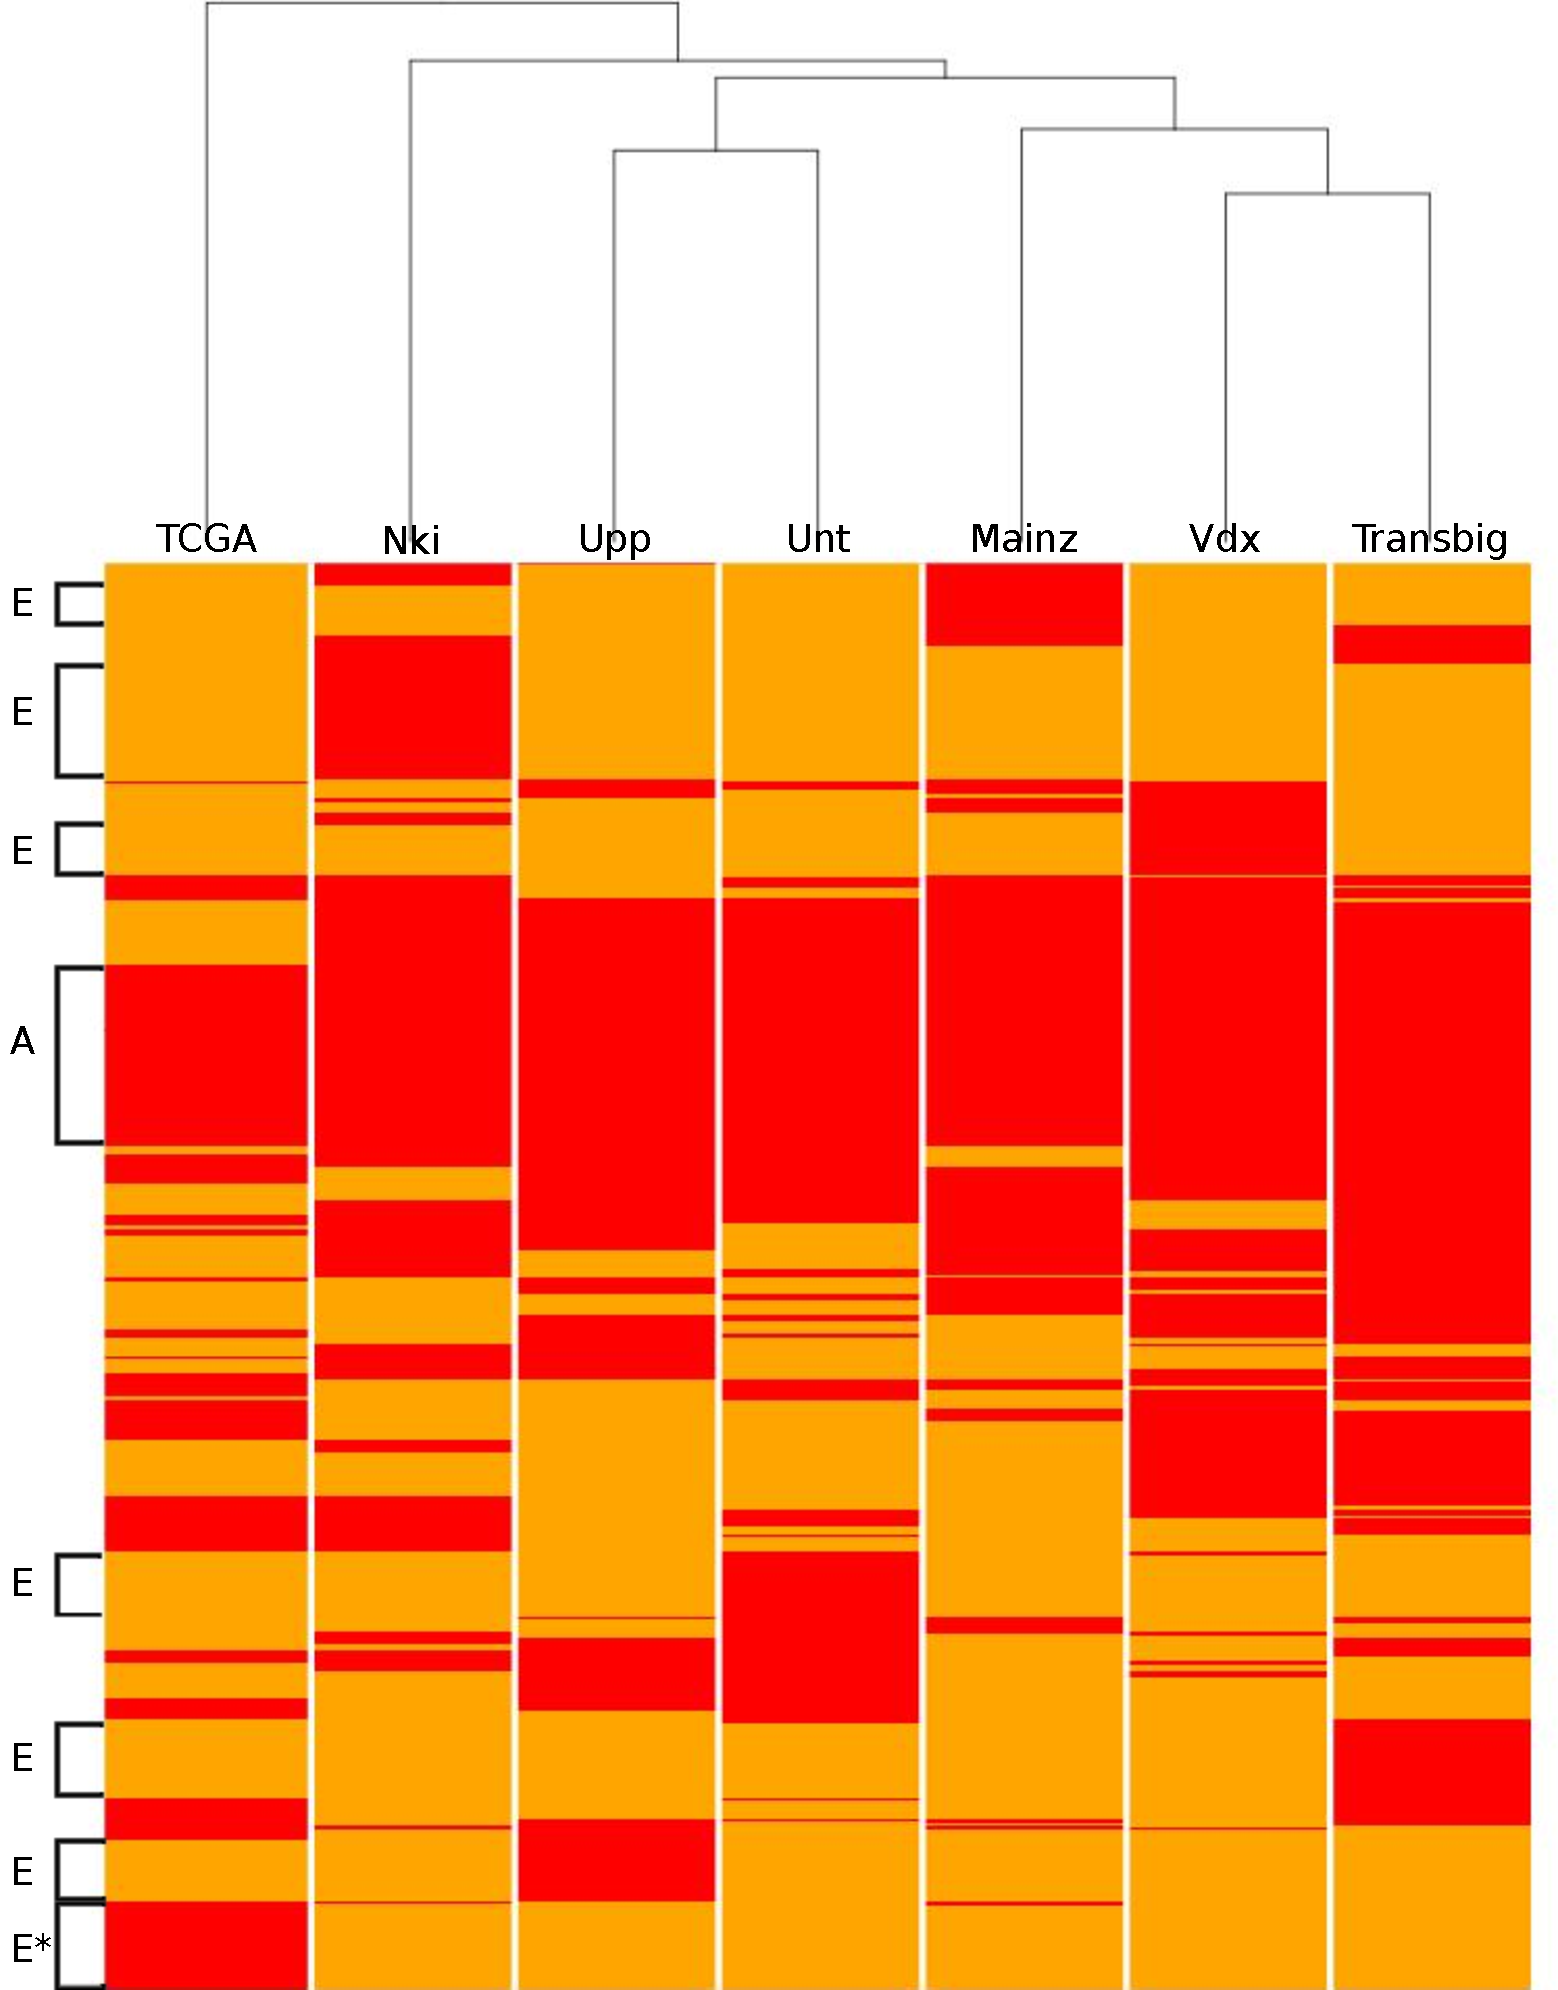
\includegraphics[width=1\linewidth]{images/IFA_FIG5} 

}

\caption{Heatmap de enriquecimiento del Análisis Funcional Integrador en cáncer de mama (incluyendo TCGA). Los datasets se ubican en columnas; y los conjuntos de genes (términos), enriquecidos en al menos un dataset, se presentan en filas. Celdas rojas indican enriquecimiento, y las anaranjadas indican que no hay enriquecimiento. Se observan subconjuntos concordantes de términos enriquecidos entre cada conjunto de datos (\textbf{A}) y subconjuntos de términos enriquecidos exclusivamente en un solo conjunto de datos (\textbf{E}).}\label{fig:ifa5}
\end{figure}


\hypertarget{ifa-sobre-datasets-de-cancer-de-prostata}{%
\subsection{IFA sobre datasets de cáncer de próstata}\label{ifa-sobre-datasets-de-cancer-de-prostata}}

\par

Con el fin de verificar que los resultados del IFA no dependen de la patología analizada, sino que puede extenderse a otros escenarios, el IFA se probó sobre cuatro datasets de cáncer de próstata disponibles en el repositorio R \textbf{Bioconductor}. En total, se obtuvieron 519 sujetos de las bases de datos: 74 sujetos con cáncer de próstata benigno y 125 con tumor para Camcap; 29 benignos y 150 tumor para Taylor; 6 vs.~13 para Varambally; y 28 vs.~94 para Grasso. Para obtener alrededor del 5\% de los genes DE, se utilizaron valores de \(treatLfc\) de 0,2, 0,15, 0,2, y 0,45 para Camcap, Taylor, Varambally y Grasso, respectivamente. Para el análisis de Varambally, los p-valores de los genes no fueron ajustados, ya que se no se obtuvieron genes DE bajo ningún valor de \(treatLfc\) con un valor de corte de FDR fijado en 0,01.

\par

La matriz de consenso resultante se muestra en la Figura \ref{fig:ifa5}, en la que 163 términos fueron enriquecidos en al menos el 80\% de los conjuntos de datos, de los cuales 99 (61\%) están relacionados con el cáncer de próstata según la BDTC. En particular, la proporción media de términos exclusivamente enriquecidos presentes en la BDTC en cada conjunto de datos fue del 44\%, con Taylor primero con 448 términos exclusivos (194 en la BDTC) y Varambally último con 212 términos (98 en la BDTC).

\newpage
\begin{figure}

{\centering 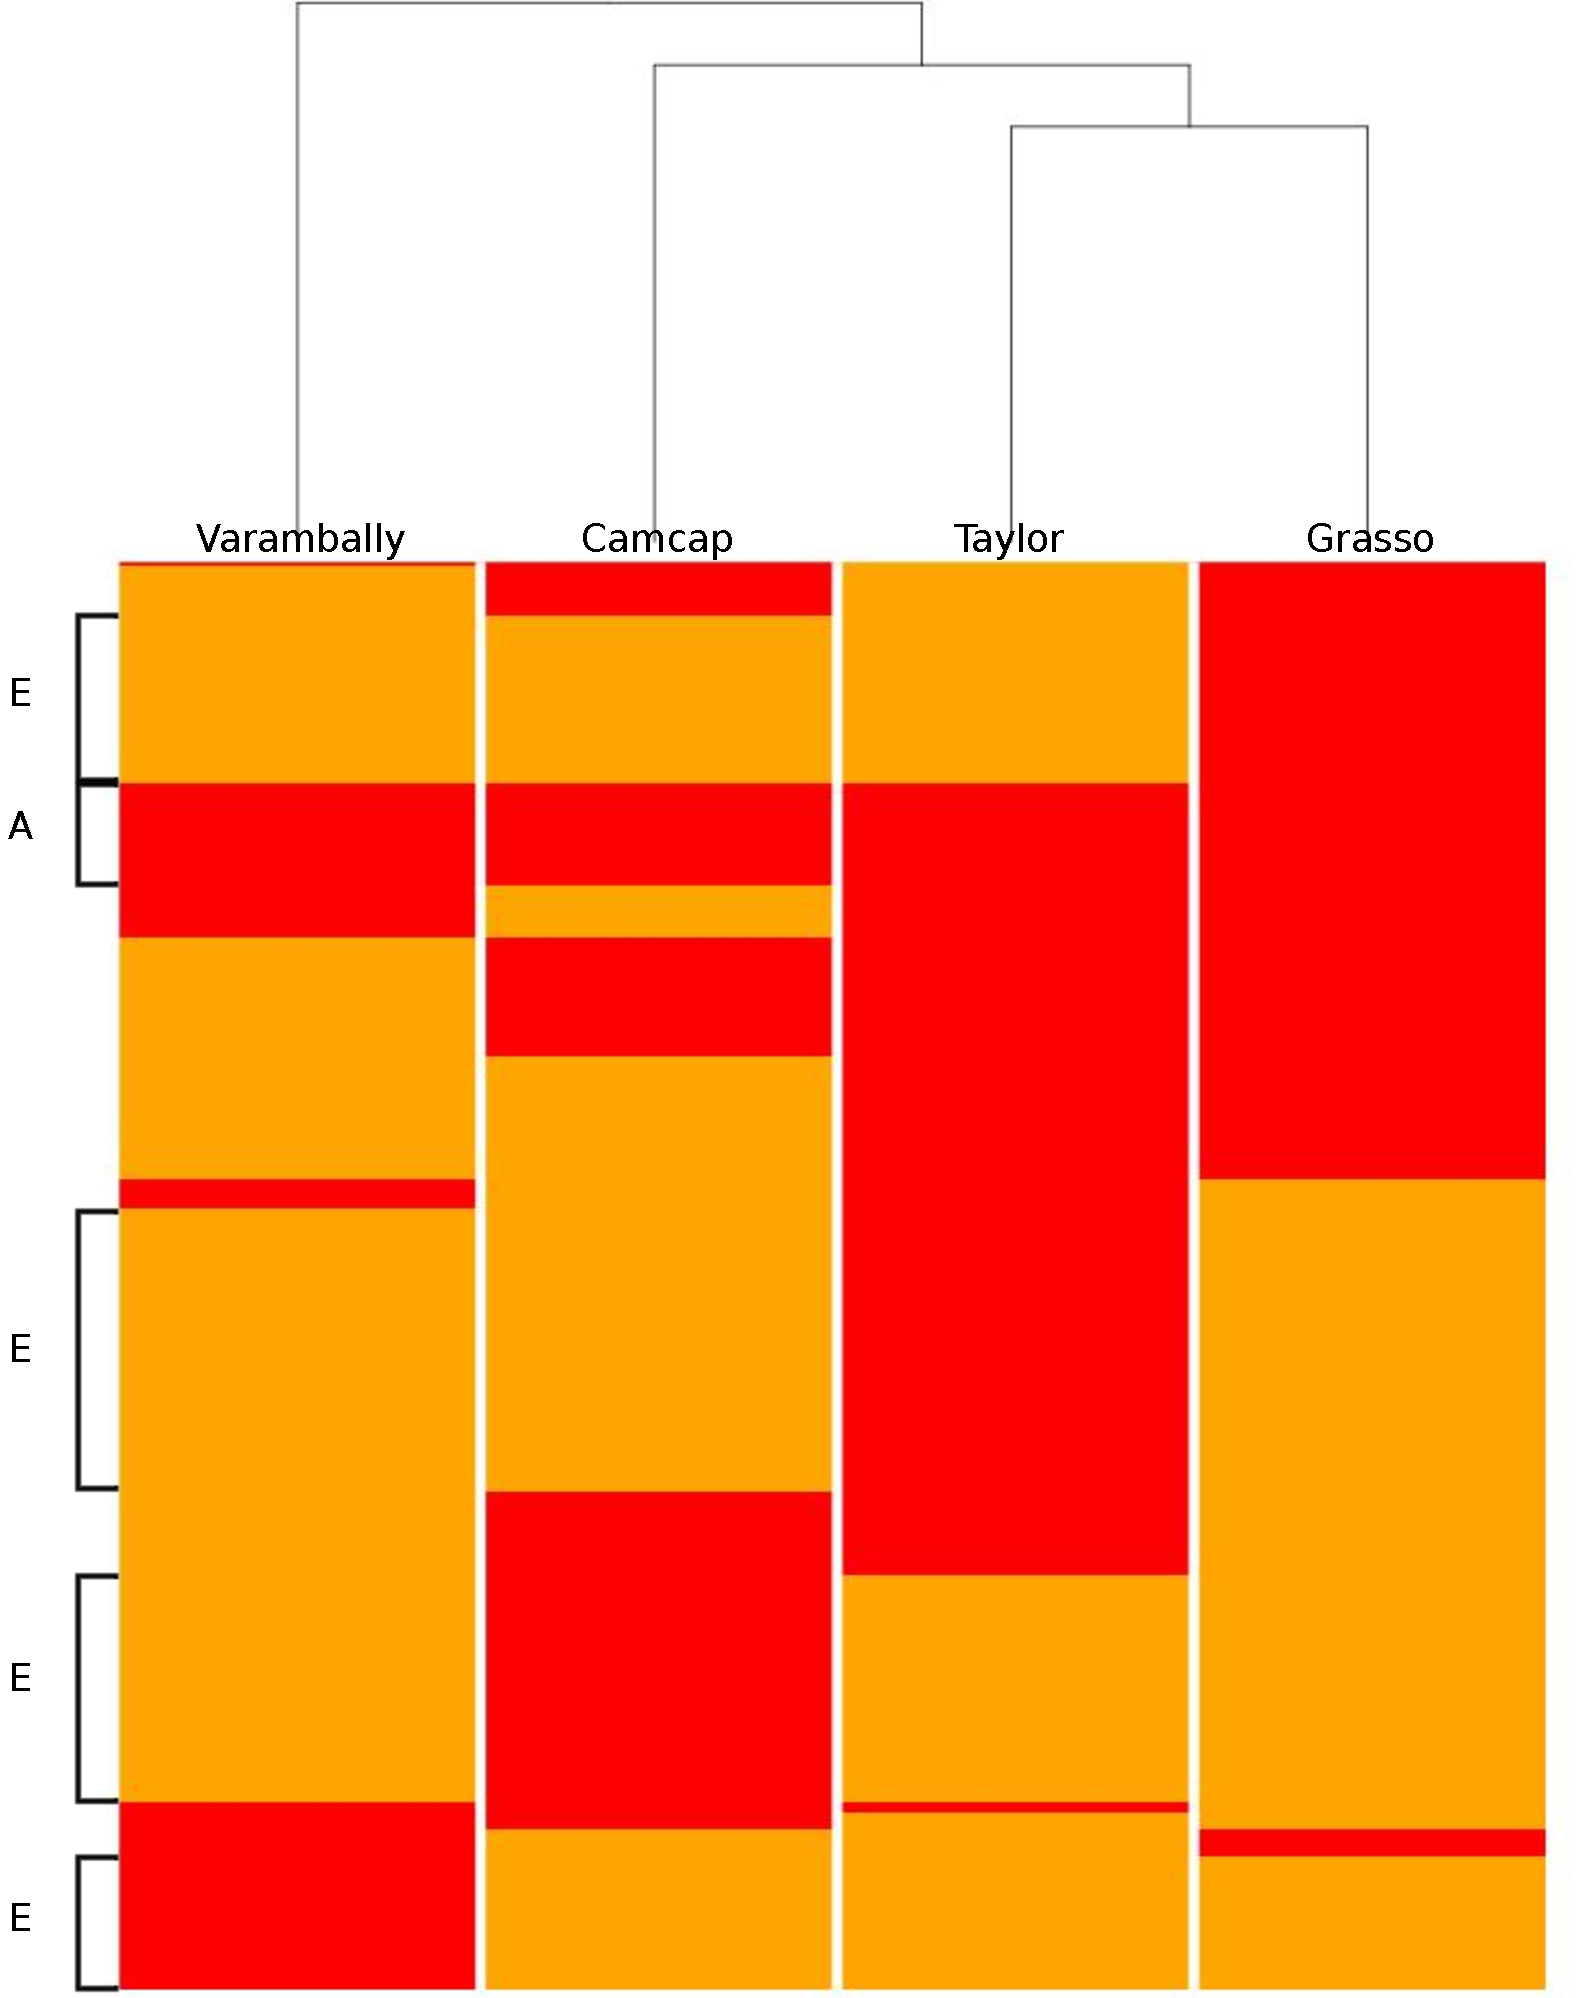
\includegraphics[width=1\linewidth]{images/IFA_FIG6} 

}

\caption{Heatmap de enriquecimiento del Análisis Funcional Integrador en cáncer de próstata. Los datasets se ubican en columnas; y los conjuntos de genes (términos), enriquecidos en al menos un dataset, se presentan en filas. Celdas rojas indican enriquecimiento, y las anaranjadas indican que no hay enriquecimiento. Se observan subconjuntos concordantes de términos enriquecidos entre cada conjunto de datos (\textbf{A}) y subconjuntos de términos enriquecidos exclusivamente en un solo conjunto de datos (\textbf{E}).}\label{fig:ifa6}
\end{figure}


\hypertarget{conclusiones}{%
\section{Conclusiones}\label{conclusiones}}

\hypertarget{comparacion-de-metodos}{%
\subsection{Comparación de métodos}\label{comparacion-de-metodos}}

\par

En este capítulo se pudo mostrar que los resultados del AF pueden varían dependiendo del método y los parámetros utilizados. Esto podría influir negativamente en la interpretación biológica si no se aborda adecuadamente. Por ejemplo, el método de PFC Subramanian mostró una alta sensibilidad a diferentes configuraciones de parámetros y datos de entrada. Los métodos SMpp0 y SMpr, utilizando el valor de corte estadístico recomendado, casi no devolvieron términos enriquecidos para los conjuntos de datos analizados. Estos resultados fueron bastante inesperados porque la naturaleza de los subtipos de cáncer de mama considerados tienen mecanismos biológicos subyacentes muy contrastantes y se han reportado resultados de supervivencia altamente opuestos (Parker et al., 2009). Sin embargo, cuando el usuario sólo tiene una lista ordenada de genes, no hay otra alternativa que la versión pre-rankeada (SMpr) para realizar PFC. En este caso, sugerimos utilizar el rankeo por \(1-p\)-\(valor\) con \(w=1\), y verificar con diversos valores de corte que devuelvan términos enriquecidos. Cuando se alimentó el SM con la matriz de expresión y sus etiquetas de fenotipo, se encontró que tanto las permutaciones de fenotipo como de genes eran muy sensibles al valor de ponderación \(w\) elegido, lo que producía diferentes cantidades de términos enriquecidos, así como diferentes niveles de variabilidad de enriquecimiento entre los conjuntos de datos. La permutación del fenotipo con \(w=2\) (SMpp2) parece proporcionar resultados estables, pero la aparición de conjuntos de datos con un número extremo de términos enriquecidos desalienta su uso. Además, cuando \(w=1\) los resultados fueron muy inestables (RIC alto). La estrategia de permutación de genes con \(w=1\) y \(w=0\) (SMgp1 y SMgp0) proporcionó resultados muy estables, pero estas parametrizaciones enriquecieron casi el doble de términos que todos los demás métodos analizados. Cuando se usó \(w=2\) (SMgp2), se obtuvo un número bajo de términos enriquecidos. En desacuerdo con los autores del SM, recomendamos SMgp sobre SMpp. Sin embargo, estamos de acuerdo con su recomendación sobre el valor de ponderación \(w=1\), es decir, recomendamos SMgp1 sobre cualquier otra configuración de SM.

\par

El método mGSZ, a comparación del SM, fue más estable entre los diversos conjuntos de datos, produciendo un alto consenso entre datasets (alto \(FCE\)) y proporcionando el mayor número de términos informativos y exclusivamente enriquecidos (\(TEE\)). Se observó que, cuando no se utilizaba límite superior de tamaño de CG (mGSZ\([5,\infty)\)), se enriquecieron términos específicos e informativos adicionales a con el límite {[}15, 500). Por lo tanto, fomentamos el uso de mGSZ\([5,\infty)\). Otra ventaja de mGSZ sobre el SM es que el primero tiene una implementación R actualizada, mientras que el segundo requiere de un entorno Java.

\par

En cuanto a las metodologías de ASR, aunque el uso de BRI produce resultados estables y contiene los términos enriquecidos utilizando BRIII, este último es más apropiado desde un punto de vista estadístico (Fresno et al., 2012). Además, se demostró que BRIII a diferencia de BRI no presenta un número extremo de términos enriquecidos, pero tiene un rango más variable de términos enriquecidos sobre los conjuntos de datos utilizados. La versión R implementada de DAVID (RD) fue desarrollada para funcionar lo más similar posible a la plataforma web de DAVID (WD), con la ventaja de utilizar una base de datos de anotaciones GO actualizada. Aún más, cualquier CG deseado de interés puede ser analizado. Además, RD no requiere una conexión a Internet ni una cuenta registrada en el sitio web de DAVID. En el caso de GOstats, se demostró que es demasiado variable cuando se prueba el enriquecimiento a través de bases de datos (bajo \(FCE\)). Esto podría volverse problemático cuando se analiza un solo conjunto de datos, es decir, daría una visión biológica muy limitada del experimento que se está analizando. Para las diversas parametrizaciones de dEnricher, se obtuvieron valores extremos de enriquecimiento cuando se utilizó test \emph{Hipergeométrico} o \emph{Binomial}; sin embargo, cuando se utilizó la prueba de \emph{Fisher}, se obtuvieron resultados concordantes. Además, al no aplicar ningún algoritmo de penalización (dE\_F\_none) se obtuvieron términos adicionales relacionados con la enfermedad bajo estudio. El dE\_F\_none resultó ser el método más estable entre los conjuntos de datos para las alternativas de ASR (el más alto \(FCE\)) y superó a sus competidores en cuanto al número de términos informativos enriquecidos exclusivamente (\(TEE_m\)).

\par

En resumen, concluimos que si los parámetros se establecen correctamente, el AF obtiene información biológica consensuada y significativa a pesar del bajo nivel de genes DE en común entre diversas bases de datos. Se demostró que tanto el ASR como la PFC proporcionan resultados complementarios que pueden integrarse para obtener una visión biológica más amplia. Además, su integración nos permite abarcar una mayor profundidad de la estructura GO, una característica deseable a la hora de contrastar condiciones experimentales (Fresno et al., 2012). En consecuencia, proponemos utilizar el pipeline del IFA, que realiza análisis simultáneos de ASR y PFC a través de dE\_F\_none y mGSZ, que resultaron ser los métodos más efectivos respectivamente. Ambos enfoques se basan en el mismo modelo lineal a través de la conocida librería R \texttt{limma} (Berkeley, 2004). Por lo tanto, proporciona un marco completo y unificado que utiliza únicamente la matriz de expresión, el diseño experimental y (si no se dispone de CG) la base de datos GO de \texttt{org.Hs.eg.db} (Carlson et al., 2013). Aunque este trabajo se basó en los conjuntos de genes GO, cualquier otra base de conocimiento de conjuntos de genes podría ser aplicada para el IFA.

\hypertarget{aplicacion-del-ifa}{%
\subsection{Aplicación del IFA}\label{aplicacion-del-ifa}}

\par

La aplicación del IFA para estudiar los términos regulados diferencialmente entre los subtipos de cáncer de mama Luminal A y Basal resultó en la detección de varios términos altamente relacionados con el cáncer de mama. Por ejemplo, IFA permitió detectar términos relacionados con las vías de señalización de los receptores de hormonas y estrógenos, los cuales están fuertemente relacionados con los subtipos de cáncer de mama analizados, ya que los sujetos Luminal A son dependientes de estrógeno, mientras que los sujetos Basales no lo son (Bastien et al., 2012; Dai et al., 2015; Goldhirsch et al., 2013). A partir del IFA, los resultados concordantes revelaron términos asociados con el proceso de desenrollado del ADN, un evento asociado con el inicio de la síntesis de ADN y relacionado con la facilitación de la actividad de las helicasas. Se ha reportado que la helicasa BACH1/FANCJ está mutada en el cáncer de mama de inicio temprano, especialmente relacionado con el gen hereditario del cáncer de mama \emph{BRCA1} (Cantor et al., 2001). La mayoría de los cánceres de mama relacionados con el gen \emph{BRCA1} son triplemente negativos y Basales (Atchley et al., 2008), por lo tanto son esperadas las diferencias en los genes que regulan el proceso de desenrollado del ADN entre Luminal A y Basal. Además, el IFA reveló un grupo de términos que sólo estaban regulados de forma diferencial en el conjunto de datos de TCGA. De ellos, la actividad de la histona metiltransferasa en H3-K9 fue uno de los términos más profundos encontrados en la estructura de árbol de GO. La metilación de la histona H3-K9 se ha correlacionado con la formación de heterocromatina y la represión transcripcional, que puede regular la expresión del receptor de estrógeno (Sharma et al., 2005). Además, el término de actividad de la tirosina cinasa está involucrada en la terapia de elusión en cánceres de mama triplemente negativos - Basales - (Scaltriti, Elkabets, \& Baselga, 2016). La evaluación de la capacidad de generalización del IFA en los conjuntos de datos sobre el cáncer de próstata también arrojó resultados concordantes e informativos. Además, como era de esperar y visto en el caso del cáncer de mama, se enriquecieron términos presentes en consenso entre los conjuntos de datos, así como términos específicos enriquecidos para cada uno de ellos.

\par

Estos hallazgos apoyan la utilidad de nuestra propuesta desde la perspectiva de la minería de datos biológicos. Además, el marco de análisis propuesto, IFA, supera las limitaciones de las bases de conocimiento que presentan los métodos, minimiza los parámetros a definir por el usuario, facilita el AF, permite la comparación de diferentes cohortes de pacientes, como se muestra con los resultados de TCGA y cáncer de próstata, y se proporciona gratuitamente como código abierto R en \href{http://github.com/jcrodriguez1989/IFA}{GitHub}.

\hypertarget{cap:migsa}{%
\chapter{Análisis masivo e integrador de conjuntos de genes}\label{cap:migsa}}

\hypertarget{motivacion-1}{%
\section{Motivación}\label{motivacion-1}}

\par

El surgimiento y rápido avance de las tecnologías de secuenciación de alto rendimiento han llevado a la disponibilidad de miles de experimentos en repositorios públicos como son el Gene Expression Omnibus (Barrett et al., 2012) y Array Express (Kolesnikov et al., 2014). Más aún, se han llevado a cabo varios proyectos de gran escala, centrados en la comprensión integrada de la complejidad de las enfermedades humanas, como The Cancer Genome Atlas (TCGA) (Weinstein et al., 2013) y el US-LACRN (Llera et al., 2015) para el estudio del cáncer. Comúnmente, los conjuntos de datos disponibles incluyen diferentes tipos de datos provenientes de múltiples tecnologías ómicas para los mismos sujetos, proporcionando información a diferentes niveles moleculares y creando oportunidades sin precedentes para estudiar enfermedades humanas. La integración de estos datos genéticos, genómicos y proteómicos puede conducir a una mejor identificación de grupos homogéneos de sujetos, así como de patrones biológicos comunes y distintivos entre los grupos. La caracterización de grupos de sujetos que presentan una misma condición patológica, contribuye al desarrollo de estrategias diagnósticas y de tratamiento más adecuadas (Chen \& Snyder, 2013; Kedaigle \& Fraenkel, 2018). En este sentido, el auge de la medicina personalizada y la disponibilidad de repositorios de datos moleculares de alto rendimiento han aumentado la necesidad de herramientas adecuadas que permitan a los investigadores traslacionales gestionar y explorar estas fuentes de datos (Canuel, Rance, Avillach, Degoulet, \& Burgun, 2014; Fernandez \& Casares, 2018).

\par

La integración y el análisis de grandes conjuntos de datos provenientes de múltiples fuentes ómicas se ha convertido en una tarea cada vez más desafiante. Los primeros esfuerzos para identificar patrones distintivos relacionados con fenotipos o contrastes (comparaciones entre pares de fenotipos) específicos se han basado en el análisis de expresión diferencial. Estos esfuerzos condujeron a la identificación de diferentes listas de genes, proteínas u otras características genómicas, con una \emph{ligera superposición} entre los conjuntos de datos (Creighton et al., 2018; Hoadley et al., 2014; Korkola et al., 2007; Meng, Kuster, Culhane, \& Gholami, 2014; Metzger Filho, Ignatiadis, \& Sotiriou, 2011; Rodriguez et al., 2016a; Verhaak et al., 2010; Weinstein et al., 2013). Por el contrario, cuando la estrategia de análisis se basaba en el enriquecimiento funcional, se identificaron \emph{grandes cantidades} de vías biológicas, funciones moleculares y procesos biológicos en común entre diferentes conjuntos de datos (Creighton et al., 2018; Meng et al., 2014; Rodriguez et al., 2016a). Estos resultados denotan que, a pesar de las posibles diferencias en las características ómicas probadas en varios ensayos, la biología subyacente presenta características similares, lo que lleva a resultados fenotípicos o pronósticos similares. Por lo tanto, el análisis funcional de Conjuntos de Genes (CG) resulta en un mejor enfoque para la integración de múltiples conjuntos de datos.

\par

El principal inconveniete de los análisis de expresión diferencial o de enriquecimiento funcional es la falta de integración de datos de múltiples ómicas. Esto ha motivado al surgimiento de un campo de investigación, conocido como \emph{Big Omics Analysis}, en el que la integración de tipos de datos dispares se ha vuelto cada vez más importante para capturar la heterogeneidad de los procesos biológicos (Fernandez \& Casares, 2018; Liu, Shen, \& Pan, 2016). Los enfoques recientes se basan en aprendizaje automático (Shen, Olshen, \& Ladanyi, 2009), análisis de redes (Wang et al., 2014), o fusión de patrones (Shi et al., 2017). Estas herramientas se basan principalmente en el análisis de expresión o patrones de coexpresión de un único conjunto de datos, lo que supone una gran limitación, ya que se debe contar con datos de cada ómica para cada sujeto. Además, ninguna de estas herramientas es capaz de analizar el comportamiento funcional de la enfermedad o fenotipo; y mucho menos analizar multiples cohortes (poblaciones). Si bien una herramienta ampliamente utilizada llamada PARADIGM (Vaske et al., 2010) ha sido desarrollada para analizar los aspectos funcionales de múltiples fuentes ómicas, sólo puede proporcionar información a nivel de sujetos individuales, y por lo tanto, omite el análisis de grupos de interés, fenotipos, conjuntos de datos o tecnologías ómicas.

\par

El análisis de grandes fuentes de datos ómicas resulta particularmente útil para el estudio de enfermedades heterogéneas, como el Cáncer de Mama (CM) (Korkola et al., 2007; Kwa, Makris, \& Esteva, 2017; Reis-Filho \& Pusztai, 2011). En este sentido, Perou et al. (Perou et al., 2000) definió cuatro subtipos intrínsecos de CM -introducidos en la Sección \ref{sec:bcSubt}- que presentan diferentes perfiles. Estos subtipos han sido ampliamente evaluados a través del análisis independiente de diferentes fuentes de datos incluyendo genes, expresión de microARN, variación del número de copias, y proteínas (Network \& others, 2012). Aunque estos análisis condujeron a la validación del esquema de clasificación de Perou et al., también han dado lugar a más preguntas sobre los propios subtipos. Por ejemplo, se ha descubierto que los sujetos con CM están agrupados en aún más grupos de subtipos (Curtis et al., 2012). Más aún, se han identificado nuevos grupos de CM dentro de los subtipos previamente definidos (Aure et al., 2017). Asimismo, algunos sujetos con CM no pudieron ser asignados a ningún subtipo existente (Fresno et al., 2016). Por lo tanto, el éxito de la medicina traslacional en CM aún se ve limitado por la capacidad de las herramientas de análisis integradoras y masivas para descifrar los procesos biológicos aún desconocidos que subyacen a cada uno de estos subtipos de CM. Para lograr este éxito, resulta fundamental una herramienta que permita al investigador comparar bases de datos tanto de diversas fuentes ómicas como de diversas poblaciones o incluso enfermedades.

\hypertarget{sec:voom}{%
\section{Adaptación del IFA a otras fuentes de datos}\label{sec:voom}}

\par

Como se mencionó en la Sección \ref{sec:ifa}, el pipeline del IFA lleva a cabo sus análisis utilizando los métodos dE\_F\_none y mGSZ. Para llevar a cabo dichos análisis, la lista de genes Diferencialmente Expresados (DE) y el rankeo son calculados mediante un modelo lineal obtenido por la función \texttt{eBayes} de la librería \texttt{limma} de R. La obtención de los genes DE se lleva a cabo como un paso anterior a utilizar dE\_F\_none, sin embargo, para el caso de mGSZ, el rankeo de los genes se realiza internamente por dicha librería.

\par

El ajuste del modelo lineal de \texttt{eBayes} asume que los datos de entrada siguen una distribución \emph{Normal}, lo cual, como se vió en la Sección \ref{sec:technols}, se cumple para datos provenientes de microarreglos de ADN y de iTRAQ. Sin embargo, este supuesto no se cumple para datos de Secuenciación de ARN, donde vimos que, al ser datos de conteos, se asemejan a una distribución de \emph{Poisson} o \emph{Binomial Negativa}.

\par

Dado el interés de desarrollar una herramienta que permita comparar, desde un punto de vista funcional, una cantidad masiva de bases de datos, tanto de diversas poblaciones como de una variedad de fuentes ómicas. Es por esto que resultó necesario adaptar el pipeline previo del IFA de modo que permita llevar a cabo el análisis a partir de datos de conteos. En particular, se debió inspeccionar el paquete R \texttt{mGSZ} y realizarle las modificaciones pertinentes sobre la metodología de rankeo de genes.

\par

El IFA utiliza una misma herramienta (y modelo estadístico), tanto para el ASR como para el análisis de PFC, para lograr un análisis unificado. La adaptación del IFA a datos de conteos se realizó manteniendo esta idea de unificación. En este sentido, tanto para la obtención de los genes DE como para rankearlos, se implementó una modificación del pipeline IFA que dependiendo del tipo de datos de entrada utiliza la función \texttt{eBayes} (para datos \emph{Normales}) ó \texttt{voom} (para conteos). La función \texttt{voom} también se encuentra desarrollada en la librería \texttt{limma}, y se desarrolló principalmente con el fin de detectar genes DE para datos de conteos, la idea de esta propuesta es poder modelar los datos como si fueran \emph{Normales} mediante mínimos cuadrados generalizados (Law, Chen, Shi, \& Smyth, 2014). Para ello se realiza una transformación sobre los datos de conteos de manera de poder corregir la relación media-varianza de los datos, a partir de un ajuste \emph{loess}. De esta manera, a partir de la matriz de conteos se obtiene una matriz de pesos asociada a la corrección necesaria y por consiguiente poder ajustar el modelo lineal mediante mínimos cuadrados generalizados. Como resultado de esta reimplementación, se obtuvo una alternativa del IFA que, de un modo transparente al usuario, permite llevar a cabo el análisis a partir tanto de datos \emph{Normales} como de conteos.

\hypertarget{herramienta-desarrollada}{%
\section{Herramienta desarrollada}\label{herramienta-desarrollada}}

\par

En el presente capítulo se introduce la librería R desarrollada: MIGSA -del inglés \emph{Massive and Integrative Gene Set Analysis}-. MIGSA tiene como objetivo identificar la presencia de patrones funcionales comunes o distintivos de diversos fenotipos. Para el análisis, los términos biológicos, clínicos, o definidos por el usuario (de interés específico) se definen mediante CG. MIGSA permite a los usuarios realizar un análisis comparativo integrador de los datasets combinando diferentes experimentos de diferentes plataformas ómicas. Nuestra librería supera la pérdida de información producida por la fusión de diferentes fuentes de datos, explota la complementariedad de los diferentes niveles ómicos y permite realizar consultas directas y supervisadas basadas en cada fenotipo.

\par

Como se explica esquemáticamente en la Figura \ref{fig:migsa1}, MIGSA toma como entrada una lista de matrices de expresión (\(L=\{M_d\}; d \in \{1,\ldots,D\}\)). Cada matriz contiene datos del \(d\)-ésimo dataset, con \(S_d\) sujetos medidos a través de cualquier tecnología ómica (por ejemplo, genes, proteínas, etc.) que pueda ser anotada con identificadores \emph{Entrez}. Para el \(d\)-ésimo conjunto de datos, MIGSA requiere la identificación del fenotipo de cada sujeto \(F_d=[f_{d1},...,f_{dS_d}]\), con \(f_{di} \in \{a,b,...\}\) \((i\in \{1,...,S_d\})\), para identificar cada experimento \(E_{d}^{a,b}\) que resulta de la matriz de expresión \(M_d\) y el contraste de fenotipo \emph{a vs.~b}. Luego, en paralelo, MIGSA aplica individualmente a cada experimento el Análisis Funcional Integrador (IFA) descrito en el Cápitulo \protect\hyperlink{cap:ifa}{3}. Vale la pena mencionar que el IFA aplicado por MIGSA presenta dos novedades respecto a su publicación original (Rodriguez et al., 2016a): ahora permite analizar datos de conteos (como los de secuenciación de ARN), microarreglos de ADN, y proteómicos de iTRAQ; e identifica los genes específicos que contribuyeron al enriquecimiento de cada CG.
\begin{figure}

{\centering 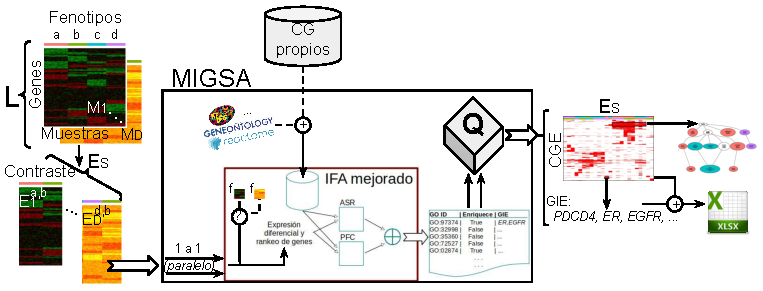
\includegraphics[width=1\linewidth]{images/MIGSA_FIG1_es} 

}

\caption{Flujo de trabajo del Análisis Masivo e Integrador de Conjuntos de Genes (MIGSA). De una lista de matrices de expresión \(L=\{M_1,....,M_D\}\), cada matriz con la identificación del fenotipo (por ejemplo \(a\), \(b\), \(c\), \(d\)) para cada muestra, se realiza la lista de experimentos (Es), donde cada experimento compara un par de fenotipos de una matriz (por ejemplo \(E_{1}^{a,b}\) contrasta los fenotipos \(a\) y \(b\) para la matriz de expresión \(M_1\)). MIGSA toma como entrada esta lista de Es y aplica, individualmente a cada experimento, una versión mejorada del IFA previamente presentado, de manera paralela. Esta versión mejorada del IFA toma una matriz de expresión y, de acuerdo con su tipo de datos, utiliza una función \(f\) diferente para obtener tanto la expresión diferencial como el rankeo de los genes, y luego realiza ambos Análisis de Sobre-Representación (ASR) y de Puntuación Funcional de Clase (FCS). Para este paso, se puede utilizar una colección generada por el usuario de conjuntos de genes ó seleccionar entre más de 130 colecciones proporcionadas por MIGSA. Los resultados de cada experimento se almacenan en un cubo de datos Q. Como salida, MIGSA proporciona diferentes alternativas de exploración y visualización, permitiendo identificar fácilmente los Conjuntos de Genes Enriquecidos (CGE) para cada experimento y, para cada conjunto de genes, los Genes Importantes para su Enriquecimiento (GIE).}\label{fig:migsa1}
\end{figure}


\par

Los resultados de MIGSA se resumen en un cubo de datos tridimensional, \(Q^{Es,CGE,GIE}\), con tres ejes o niveles de abstracción: Experimentos (Es; es decir, contrastes de fenotipos), Conjuntos de Genes Enriquecidos (CGE; CG estadísticamente desregulados para un umbral de significancia), y la lista de Genes Importantes para el Enriquecimiento (GIE; es decir, para cada CG, los genes que fueron los principales responsables de su desregulación en un experimento específico). Así, para el experimento \(E_{d}^{a,b}\), MIGSA proporciona la lista de conjuntos de genes enriquecidos \(CGE_{d}^{a,b}\), y la lista de genes importantes de enriquecimiento \(GIE_{d}^{a,b}\) (ver Figura \ref{fig:migsa1}). Nótese que en el cubo \(Q\) los ejes son: \(Es=\cup_d\cup_{a,b}E_{d}^{a,b}\), \(CGE=\cup_d\cup_{a,b}CGE_{d}^{a,b}\), y \(GIE=\cup_d\cup_{a,b}GIE_{d}^{a,b}\).

\par

Un gen \(G\) será considerado un GIE para un determinado conjunto de genes \(CG\) y experimento \(E_{d}^{a,b}\), si \(G \in CG\), y al menos uno de:
\begin{itemize}
\tightlist
\item
  \(CG\) fue enriquecido por el análisis de sobre-representación, y el gen \(G\) se encontró diferencialmente expresado en \(E_{d}^{a,b}\).
\item
  \(CG\) fue enriquecido por puntuación funcional de clase, y el gen \(G\) conformó el \emph{leading-edge} (Subramanian et al., 2005) de \(CG\), es decir, la posición de \(G\), en el rankeo, se encuentra a la izquierda/derecha de la gráfica positiva/negativa del \emph{Enrichment Score} de \(CG\).
\end{itemize}
\par

MIGSA proporciona varias herramientas gráficas, que permiten a los usuarios explorar y visualizar fácilmente los resultados de sus datos. Por ejemplo, el primer eje del cubo MIGSA (\(Q^{CGE,Es}\)) puede representarse fácilmente mediante un \emph{heatmap}. En este caso, los CG se distribuyen en filas y los experimentos en columnas. En particular, las filas y columnas se encuentran ubicadas de acuerdo a un ordenamiento dado por la distancia Jaccard y enlace promedio. El \emph{heatmap} de MIGSA resume eficazmente los resultados de múltiples IFA y ofrece a los usuarios la capacidad de visualizar patrones de enriquecimiento funcional relacionados con contrastes, fenotipos o incluso con fuentes de datos específicas. El \emph{heatmap} incluye un dendrograma superior que muestra los grupos formados por los resultados de todos los experimentos. Este dendrograma permite una rápida identificación de clusters y sub-clusters de experimentos, y su asociación con los fenotipos estudiados.

\hypertarget{validacion-de-la-herramienta}{%
\section{Validación de la herramienta}\label{validacion-de-la-herramienta}}

\par

Para demostrar la utilidad de MIGSA como herramienta de descubrimiento, se utilizó con el fin de lograr una caracterización funcional de cada subtipo molecular PAM50 de CM. Se aplicó MIGSA para analizar una gran cantidad de bases de datos de CM donde se evaluaron todas las combinaciones posibles de pares de subtipos. La eficiencia de MIGSA se vería reflajada en encontrar genes y patrones funcionales que caractericen los diversos fenotipos analizados. En este sentido, dado que se analizaron experimentos pertenecientes a una misma enfermedad, será esperable encontrar patrones en común compartidos entre todos los contrastes. Pero también, y quizás de mayor interés biológico, resultará fundamental detectar patrones específicos que caractericen cada contraste, y más particularmente, cada subtipo.

\hypertarget{datos-de-entrada-1}{%
\section{Datos de entrada}\label{datos-de-entrada-1}}

\hypertarget{matrices-de-expresion-1}{%
\subsection{Matrices de expresión}\label{matrices-de-expresion-1}}

\par

Se analizaron veinticinco conjuntos de datos de expresión génica de cáncer de mama basados en microarreglos de ADN (4.145 sujetos) previamente reportados por Haibe-Kains et al. (Haibe-Kains et al., 2012) e identificados como \emph{microarreglos comerciales} por Fresno et al. (Fresno et al., 2016), estos conjuntos de datos son los de CM presentes en la Tabla \ref{tab:databases}, excepto por los de TCGA. Para cada sujeto de los datasets de Haibe-Kains (HKds), se tomó la clasificación PAM50 basada en el algoritmo \texttt{pbcmc}, según se detalla en Fresno et al.~El algoritmo \texttt{pbcmc} devuelve un nivel de confianza de que un sujeto efectivamente pertenezca a un subtipo o no, de este modo se evita analizar sujetos que posiblemente estén mal asignados por \texttt{genefu}, y que por ende, provoquen un sesgo en los resultados. Se conservaron aquellos sujetos clasificados efectivamente como Basal, Luminal A, Luminal B y Her2+, mientras que los sujetos clasificados como Normal o No Asignados fueron descartados, lo que resultó en un total de 2.756 sujetos analizados.

\par

Además de los HKds, se analizó una población de 97 sujetos que cuentan tanto con datos transcriptómicos (secuenciación de ARN y microarreglos de ADN) y proteómicos (iTRAQ) de TCGA; se seleccionaron los mismos sujetos para cada una de las bases de datos para evitar posibles sesgos. La clasificación PAM50 para estos sujetos se obtuvo a través de la librería \texttt{pbcmc} utilizando los datos de microarreglos y la opción de estandarización de escala. Mediante \texttt{pbcmc} se obtuvieron 25, 25, 12, 20, 0, y 15 sujetos identificados como Basal, Her2+, Luminal A, Luminal B, Normal, y No Asignados, respectivamente.

\par

Para cada conjunto de datos, se promediaron los genes con múltiples sondas o detecciones. Para cada contraste de dos subtipos, sólo se incluyeron los genes detectados en al menos el 70\% de los sujetos de cada subtipo. Además, para los datos del secuenciación de ARN, sólo se incluyeron los genes con más de 10 conteos en promedio por subtipo. Para un conjunto de datos dado y para cada subtipo dado, si había menos de ocho sujetos presentes, entonces estos sujetos fueron descartados para evitar tener una población no representativa, y en consecuencia no se analizaron los contrastes con ese subtipo para ese conjunto de datos.

\par

Luego de los filtros mencionados, se obtuvieron 118 experimentos que contrastan los subtipos de CM para los HKds y 18 para TCGA. Para el análisis de sobre-representación del IFA de MIGSA, se eligieron parámetros de selección de expresión diferencial que incluyan entre el 4 y 6\% de los genes como diferencialmente expresados.

\hypertarget{conjuntos-de-genes-1}{%
\subsection{Conjuntos de genes}\label{conjuntos-de-genes-1}}

\par

MIGSA permite realizar el IFA analizando más de 130 bases de datos disponibles de CG conocidos (Kuleshov et al., 2016), como así también utilizar cualquier colección de CG especificada por el usuario. En este trabajo se obtuvieron (\texttt{org.Hs.eg.db} \emph{v3.5.0}) y analizaron las tres categorías de CG de GO (Consortium, 2016), alcanzando 15,796, 1,902, y 4,604 CG de las ontologías de Procesos Biológicos (PB), Componentes Celulares (CC), y Funciones Moleculares (FM), respectivamente. Un CG se consideró CGE si obtuvo un p-valor \(\le 0,01\) por el IFA.

\hypertarget{estrategias-para-el-analisis-de-eficiencia}{%
\section{Estrategias para el análisis de eficiencia}\label{estrategias-para-el-analisis-de-eficiencia}}

\par

Como primer instancia, se aplicó MIGSA sobre los experimentos de los HKds. Con el cubo resultante de MIGSA, se combinaron los resultados para definir los conceptos:
\begin{itemize}
\tightlist
\item
  \textbf{Términos Enriquecidos en Consenso por Contraste} (\textbf{TECC}): Para cada contraste, esos CG (y GIE) enriquecidos en al menos \emph{K}\% de los experimentos del contraste (donde \emph{K} es un nivel definido por el usuario, aquí usamos \(K=50\)), es decir, \(\boldsymbol{TECC}^{a,b}=\{CG:\sum_{j=1}^D I(CG \in CGE_j^{a,b}) \ge \frac{K}{100}N^{a,b}\}\) donde \emph{I} es la función indicadora, \emph{D} es el número de datasets (aquí \(D=25\) HKds), y \(N^{a,b}\) el es el número de experimentos que contrastan el subtipo \emph{a} con \emph{b}.
\item
  \textbf{Perfil Transcriptómico Funcional} (\textbf{PTF}): Para cada subtipo, aquellos \textbf{TECC} (y sus respectivos GIE) presentes en común al contrastar un subtipo contra cada uno de los restantes, es decir, \(\boldsymbol{PTF}_a=\cap_{b \neq a} \boldsymbol{TECC}^{a,b}\).
\end{itemize}
\par

Luego, se analizaron los \textbf{TECC} para obtener un perfil funcional para cada contraste de los subtipos de CM. Adicionalmente, se obtuvieron los \textbf{PTF} basados en los experimentos de los HKds y se exploraron conjuntamente con los GIE correspondientes, para obtener una caracterización funcional de cada subtipo de CM.

\par

Posteriormente, para demostrar la capacidad del paquete MIGSA de integrar múltiples conjuntos de datos ómicos, se aplicó MIGSA a los conjuntos de datos de TCGA de CM, y los resultados se compararon con los \textbf{TECC} definidos con los experimentos de los HKds. Para evaluar la concordancia entre los resultados de MIGSA sobre los conjuntos de datos de transcriptómica y proteómica del TCGA, se analizaron los CGE (y los GIE) para definir:
\begin{itemize}
\tightlist
\item
  \textbf{Términos Enriquecidos por Transcriptómica} (\textbf{TET}): Para cada subtipo, aquellos CG enriquecidos consistentemente en experimentos transcriptómicos. Para identificar los \textbf{TET}, primero, para cada contraste, se obtuvo la intersección de CGE tanto en los datos de secuenciación de ARN como en los de microarreglos de TCGA. Luego, para cada subtipo, el conjunto de términos presentes en los tres contrastes del subtipo dado se denominó Términos Enriquecidos por Transcriptómica.
\item
  \textbf{Términos Enriquecidos por Proteómica} (\textbf{TEP}): Para cada subtipo, aquellos CG enriquecidos consistentemente en experimentos proteómicos. Para obtener los \textbf{TEP}, primero, se identificaron los CGE encontrados en los experimentos de iTRAQ del TCGA para cada contraste. Luego, se seleccionó el conjunto de términos presentes en todos los contrastes de un subtipo dado.
\end{itemize}
\par

Finalmente, para cada subtipo, se evaluó la concordancia en la detección de CGE a través de diferentes plataformas y conjuntos de datos ómicos comparando los \textbf{TET} y \textbf{TEP} del TCGA, con los \textbf{PTF} encontrados analizando los experimentos de los HKds. Utilizando MIGSA, se llevo a cabo una inspección de los árboles de GO para encontrar intersecciones entre \textbf{PTF}, \textbf{TET} y \textbf{TEP} para las categorías de PB, FM y CC de cada subtipo.

\hypertarget{resultados-1}{%
\section{Resultados}\label{resultados-1}}

\hypertarget{migsa-sobre-datasets-de-microarreglos}{%
\subsection{MIGSA sobre datasets de microarreglos}\label{migsa-sobre-datasets-de-microarreglos}}

\par

Se analizaron, con MIGSA, los 118 experimentos de HKds. En la Figura \ref{fig:migsa2} se observa el \emph{heatmap} que ilustra el primer eje del cubo de resultados (\(Q^{CGE,Es}\)), donde el dendrograma superior revela los clusters formados por los resultados de todos los experimentos que contrastan los subtipos de CM. Al analizar los dendrogramas se nota la conformación de clusters generados principalmente por los subtipos contrastados (no se encontró efecto de lote o plataforma). En particular, el cluster más grande contiene todos los experimentos que contrastan el subtipo Luminal A (marca LA en la Figura \ref{fig:migsa2}; 63 experimentos/columnas). Dentro de este cluster, se identificaron dos sub-cluster distintos. Uno de estos sub-clusters consiste en 23 de un total de 25 (92\%) experimentos evaluando Luminal A contra Basal (marca LA-Ba). El otro sub-cluster incluyó 18 de 20 (90\%) experimentos contrastando los dos subtipos Luminales (marca LA-LB). Los experimentos que comparan Luminal A contra Her2+ (LA-H) fueron agrupados principalmente en dos clusters que contienen seis y nueve de 18 (83\%) experimentos respectivamente.

\par

El segundo gran cluster divisable en la Figura \ref{fig:migsa2} incluye todos los experimentos que contrastan los subtipos Basal con Luminal B ó Her2+ (marca Ba). En este cluster, se identificaron dos sub-clusters, uno con 15 de 20 (75\%) experimentos contrastando Basal con Luminal B (marca Ba-LB), y otro con 12 de 18 (67\%) experimentos contrastando Basal con Her2+ (marca Ba-H). Además de estos dos grandes sub-clusters, se diferencia uno con experimentos que contrastan Luminal B con Her2+ (marca LB-H), con 14 de 17 (82\%) experimentos. En particular, este último cluster tiene la menor cantidad de términos enriquecidos, lo que sugiere una gran similitud entre estos dos subtipos.
\begin{figure}

{\centering 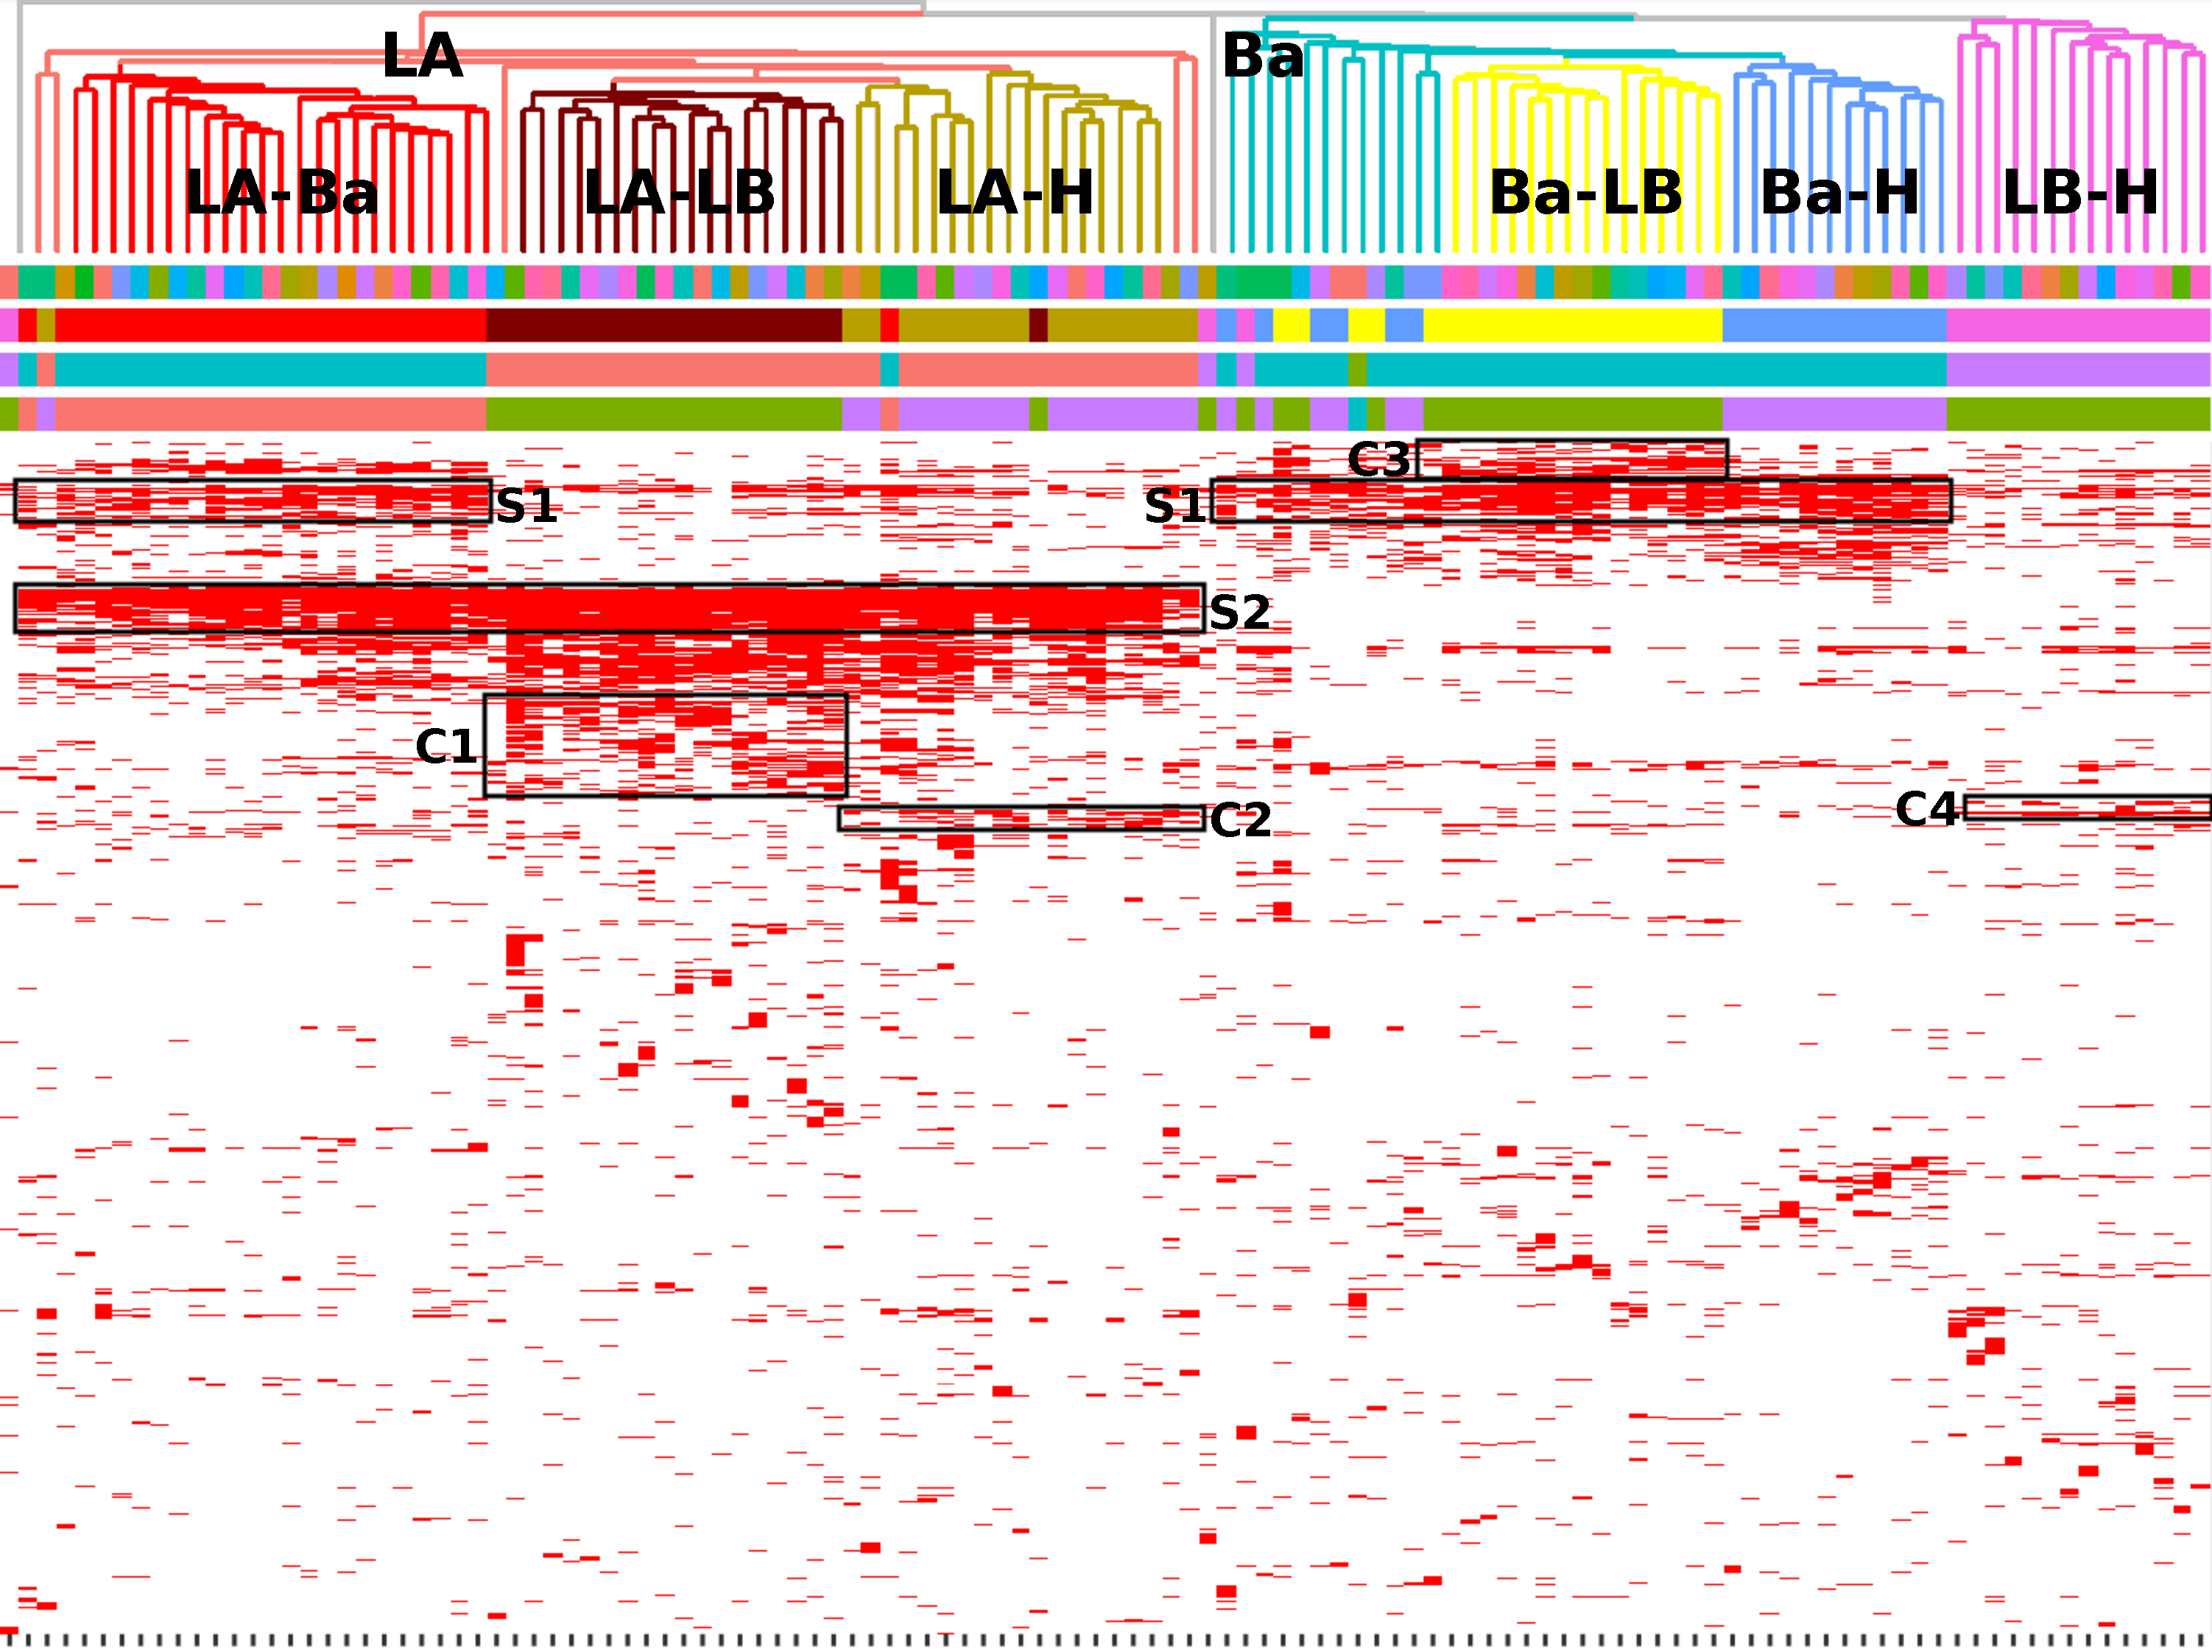
\includegraphics[width=1\linewidth]{images/MIGSA_FIG2} 

}

\caption{Conjuntos de genes enriquecidos por análisis funcional para cada experimento. Heatmap: conjuntos de genes en filas, experimentos en columnas; ordenados por distancia Jaccard y enlace promedio. Conjuntos de genes enriquecidos en rojo. Las casillas S1 y S2 contienen conjuntos de genes enriquecidos en común para subtipos, y las casillas C1, C2, C3 y C4 para contrastes (comparación entre pares de subtipos). Barras de columnas (de arriba abajo): datasets (cada color representa uno de los 25 datasets analizados); contraste; subtipo1 y subtipo2, salmón es Luminal A (LA), turquesa es Basal (Ba), púrpura es Her2+ (H), y el verde es Luminal B (LB). Clusters de dendrogramas: Se demarcan para los subtipos Basal (Ba) y Luminal A (LA), y uno por cada contraste.}\label{fig:migsa2}
\end{figure}


\par

El \emph{heatmap} de la Figura \ref{fig:migsa2} también reveló patrones de enriquecimiento comunes específicos de subtipos para todos los subtipos contrastados. Por ejemplo, las cajas S1 muestran CGE que se encuentran comúnmente en los contrastes con el subtipo Basal, mientras que la caja S2 indica patrones de enriquecimiento de Luminal A. Además, también se observan patrones de enriquecimiento específicos de contrastes, es decir, conjuntos de términos que denotan diferencias entre dos subtipos determinados. Por ejemplo, la caja C1 contiene aquellos CG que diferencian Luminal A de Luminal B, la caja C2 para Luminal A vs.~Her2+, C3 para Basal vs.~Luminal B, y C4 para Luminal B vs.~Her2+.

\par

Las capacidades exploratorias de MIGSA se utilizaron para sub-dividir el \emph{heatmap} mostrado en la Figura \ref{fig:migsa2} en \emph{sub-heatmaps} específicos de cada subtipo (es decir, Basal vs.~todos los demás, Her2+ vs.~todos los demás, Luminal B vs.~todos los demás, y Luminal A vs.~todos los demás). Estos \emph{sub-heatmap} proporcionaron una visión detallada de los patrones de enriquecimiento de cada subtipo, y pueden observarse en (Rodriguez, Merino, Llera, \& Fernández, 2019). En particular, los dendrogramas de estas figuras mostraron una mejor agrupación por contrastes, es decir, clusters para cada contraste que agruparon más experimentos que en la Figura \ref{fig:migsa2}.

\par

El número de \textbf{TECC} y de términos en \textbf{PTF} encontrados se presenta en la Tabla \ref{tab:migsa1}. Como puede observarse, el número más bajo de \textbf{TECC} (184) se encuentra para el contraste Luminal B vs.~Her2+, mientras que el contraste Luminal A vs.~Luminal B muestra el valor más alto, con 983 CG enriquecidos. En términos de los \textbf{PTF}, Luminal B y Her2+ fueron los que presentaron el menor número de términos, mientras que Luminal A alcanzó el mayor número de CG en su \textbf{PTF}, seguido por el subtipo Basal.

Cabe señalar que los \textbf{PTF} no son mutuamente excluyentes, lo cuál era de esperar ya que todos los fenotipos contrastados son subtipos de la misma enfermedad. Veintisiete CG se encontraron presentes, en común, en los \textbf{PTF} de los cuatro subtipos de CM, mientras que 506 CG fueron únicos (exclusivos) para un solo subtipo. El número de CG exclusivos observados para cada \textbf{PTF} fue de 103 para Basal, uno para Luminal B, siete para Her2+ y 395 para Luminal A. Además, se encontraron 33 CG en común entre dos \textbf{PTF} diferentes: diez en \(\boldsymbol{PTF}_{Basal} \cap \boldsymbol{PTF}_{Her2+}\), ocho en \(\boldsymbol{PTF}_{Basal} \cap \boldsymbol{PTF}_{Luminal B}\), siete en \(\boldsymbol{PTF}_{Basal} \cap \boldsymbol{PTF}_{Luminal A}\), y ocho en \(\boldsymbol{PTF}_{Luminal B} \cap \boldsymbol{PTF}_{Luminal A}\).
\begin{longtable}[]{@{}lccccc@{}}
\caption{Conjuntos de genes en consenso. Número de Términos Enriquecidos en Consenso por Contraste (\textbf{TECC}), definidos como aquellos conjuntos de genes enriquecidos en al menos el 50\% de los experimentos evaluados para cada contraste (fila vs.~columna). La columna ``Intersección'' indica el número de conjuntos de genes encontrados en todos los \textbf{TECC} de cada subtipo dado, lo cual define el Perfil Transcriptómico Funcional (\textbf{PTF}) de cada subtipo de cáncer de mama.\label{tab:migsa1}}\tabularnewline
\toprule
Contraste & Basal & Luminal B & Her2+ & Luminal A & Intersección\tabularnewline
\midrule
\endfirsthead
\toprule
Contraste & Basal & Luminal B & Her2+ & Luminal A & Intersección\tabularnewline
\midrule
\endhead
Basal & - & 488 & 437 & 768 & 155\tabularnewline
Luminal B & & - & 184 & 983 & 44\tabularnewline
Her2+ & & & - & 707 & 44\tabularnewline
Luminal A & & & & - & 437\tabularnewline
\bottomrule
\end{longtable}
\hypertarget{exploracion-de-los-ptf-de-los-subtipos-de-cancer-de-mama}{%
\subsection{Exploración de los PTF de los subtipos de cáncer de mama}\label{exploracion-de-los-ptf-de-los-subtipos-de-cancer-de-mama}}

\par

La exploración de los \textbf{PTF} reveló varios CG de GO previamente relacionados con los subtipos de CM. La visualización basada en árboles de la estructura GO, proporcionada por MIGSA, se utilizó para visualizar el \textbf{PTF} de cada subtipo en las categorías PB, CC y FM de GO. Los árboles de GO de los \textbf{PTF} de cada subtipo pueden encontrarse en (Rodriguez et al., 2019), donde cada término fue codificado por colores de acuerdo al \textbf{PTF} al que pertenece. La visualización en árbol nos permitió explorar más a fondo las relaciones entre los \textbf{PTF} de cada subtipo. La exploración de los árboles reveló que los términos no estaban dispersos al azar, sino que se encontraban conformando ramas a diversas profundidades, dominadas principalmente por subtipos particulares. Además, los CG presentes en común en los \textbf{PTF} de todos los subtipos fueron encontrados ubicados en nodos poco profundos que involucran términos generales y comúnmente encontrados, tales como citoplasma, desarrollo de sistemas, muerte y proliferación celular.

\par

El análisis del árbol de PB reveló que las ramas que involucran términos relacionados con la regulación de la vía de señalización de los receptores de estrógeno sólo aparecieron en el \textbf{PTF} del subtipo Basal. Esto está motivado por el hecho de que, genes implicados en estos CG, incluyendo \emph{ESR1}, se han encontrado previamente sobre-expresados en los subtipos Luminales y en algunos tumores Her2+ (Network \& others, 2012), y sub-expresados en los sujetos Basal (Valentin, Da Silva, Privat, Alaoui-Jamali, \& Bignon, 2012). Por esta razon, estos términos no se encontraron entre los \textbf{TECC} de los contrastes que involucran a los subtipos Luminales y HER2+ y, en consecuencia, no estaban presentes en el \textbf{PTF} de estos subtipos. Además, los términos asociados con el filamento de actina, la transición epitelio-mesénquima y el estrés del retículo endoplásmico aparecieron en el árbol de PB como \textbf{PTF} de Basal. Estas ramas son procesos bien conocidos relacionados con los tumores Basales, que los diferencian de otros subtipos (Guen et al., 2017). Los genes \emph{MLPH} y \emph{FOXC1} se encontraron entre los GIE presentes en estas ramas, y fueron consistentemente sub y sobre-expresados, respectivamente, en todos los experimentos en los que se contrastó Basal. Cabe mencionar que estos dos genes están involucrados en una firma molecular recientemente desarrollada para cánceres de mama triple negativos, altamente relacionados con tumores Basales (Santuario-Facio et al., 2017). Además, los GIE presentes en términos relacionados con la diferenciación celular, como \emph{GATA3} y \emph{FOXA1}, se encontraron desregulados en el subtipo Basal para todos los contrastes evaluados, en concordancia con los hallazgos del ``Grupo del Atlas del Genoma del Cáncer'' (Network \& others, 2012). A su vez, \emph{ERBB4}, un oncogén drogable (un gen cuya expresión puede afectarse con drogas), se encontró desregulado en el 95\% de los contrastes con Basal evaluados, lo que sugiere que los sujetos Basales no se verían afectados por los fármacos que ataquen el gen \emph{ERBB4}.

\par

El subtipo Luminal A resultó ser muy diferente de los demás en lo que se refiere a los procesos de regulación del ciclo celular y replicación del ADN, en donde los términos como la transición G1/S del ciclo celular y la unión del origen de la replicación del ADN aparecieron como su \textbf{PTF}. Es bien sabido que los procesos de progresión a través del ciclo celular y la replicación del ADN están profundamente involucrados en la proliferación (Hanahan \& Weinberg, 2000), que es la principal diferencia entre Luminal A y los subtipos más agresivos como Luminal B, Her2+, y Basal (Prat \& Perou, 2011; Yersal \& Barutca, 2014). En particular, estos términos muestran la principal diferencia entre los dos subtipos Luminales, ya que los tumores Luminal B expresan clásicamente niveles más altos de Ki67 (Cheang et al., 2009). Adicionalmente, se encontró que los GIE que provocan la proliferación celular, tales como \emph{AURKA}, \emph{PCNA}, \emph{CHEK2}, y \emph{RAD51}, estaban sub-expresados en Luminal A con respecto a los otros subtipos. Mientras que, genes como \emph{ERBB2}, \emph{GRB7}, y \emph{FGFR4} fueron encontrados sobre-expresados en todos los experimentos en los que Her2+ fue contrastado, en concordancia con lo informado por el ``Grupo del Atlas del Genoma del Cáncer'' (Network \& others, 2012).

\hypertarget{integracion-de-resultados-de-migsa-de-tcga-y-haibe-kains}{%
\subsection{Integración de resultados de MIGSA de TCGA y Haibe-Kains}\label{integracion-de-resultados-de-migsa-de-tcga-y-haibe-kains}}

\par

Los resultados de MIGSA para cada tecnología de expresión del TCGA se combinaron con los resultados de los HKds. La Figura \ref{fig:migsa3} muestra el \emph{heatmap} del eje \(Q^{CGE,Es}\) del cubo de resultados de MIGSA. El análisis del dendrograma superior mostró que los contrastes evaluados a partir de los datos del TCGA se asemejan a los respectivos resultados de HKds.

\par

Como en la Figura \ref{fig:migsa2}, al analizar la Figura \ref{fig:migsa3} se encontró un gran cluster con 11 de 12 experimentos contrastando Luminal A (marca LA), y otro cluster incluyendo los ocho experimentos contrastando el subtipo Basal con Luminal B ó Her2+ (marca Ba). Curiosamente, ambos clusters identificados contienen un cluster más específico, que agrupa únicamente experimentos transcriptómicos (marcas LA\(^T\) y Ba\(^T\)). Además, para cada contraste, se encontró un cluster que agrupaba solamente datos transcriptómicos, es decir, de microarreglos y secuenciación de ARN del TCGA, junto con los \textbf{TECC} de HKds (marcas T). Este resultado se encuentra en acuerdo con lo reportado por el ``Grupo del Atlas del Genoma del Cáncer'' (Network \& others, 2012) para un subgrupo de sujetos Luminal B y Her2+. En concordancia con los resultados del ``Grupo del Atlas del Genoma del Cáncer'' para arrays de proteínas en fase inversa (Network \& others, 2012), los experimentos proteómicos que contrastan Basal con Luminal B ó Her2+ se agruparon cerca de sus contrapartes transcriptómicas. Por otro lado, para los demás contrastes, la expresión de proteínas parece proporcionar información funcional complementaria a su contraparte transcriptómica.

\par

Para cada subtipo, se obtuvieron los \textbf{TET} y los \textbf{TEP}, y los correspondientes GIE, y se analizaron en conjunto con los correspondientes \textbf{PTF} encontrados previamente. En la Tabla \ref{tab:migsa2}, para cada subtipo, se presenta el número de términos que se encuentran exclusivamente en \textbf{PTF}, \textbf{TET} y \textbf{TEP}, y los que se encuentran exclusivamente en cada intersección. Analizando estos los resultados, encontramos que la concordancia entre los \textbf{PTF} y su contraparte del TCGA es notable. Por ejemplo, de los 680 términos que pertenecen a los \textbf{PTF} (suma de celdas de la fila Total para columnas que involucran los \textbf{PTF}), el 38\% también se encontró en \textbf{TEP} o \textbf{TET} de los datos del TCGA. En particular, los subtipos Basal y Luminal A fueron los únicos que exhibieron términos en común entre transcriptómica (\textbf{PTF} y \textbf{TET}) y proteómica (\textbf{TEP}). También se encontró que casi el 80\% de esos términos en los \textbf{TET} también se encontraron en los \textbf{PTF}, evidenciando la alta consistencia de MIGSA para analizar los conjuntos de datos de transcriptómica de los HKds y TCGA. Por el contrario, y para todos los subtipos de CM, esos términos enriquecidos con datos proteómicos no se encontraron frecuentemente entre los \textbf{TET}. Este hallazgo sugiere que los \textbf{TEP} proporcionan información complementaria a la contraparte transcriptómica, como se reportó previamente (Meng et al., 2014). Sin embargo, será necesaria una investigación más profunda que incluya un mayor número de datasets proteómicos para poder definir un Perfil \textbf{Proteómico} Funcional.
\begin{figure}

{\centering 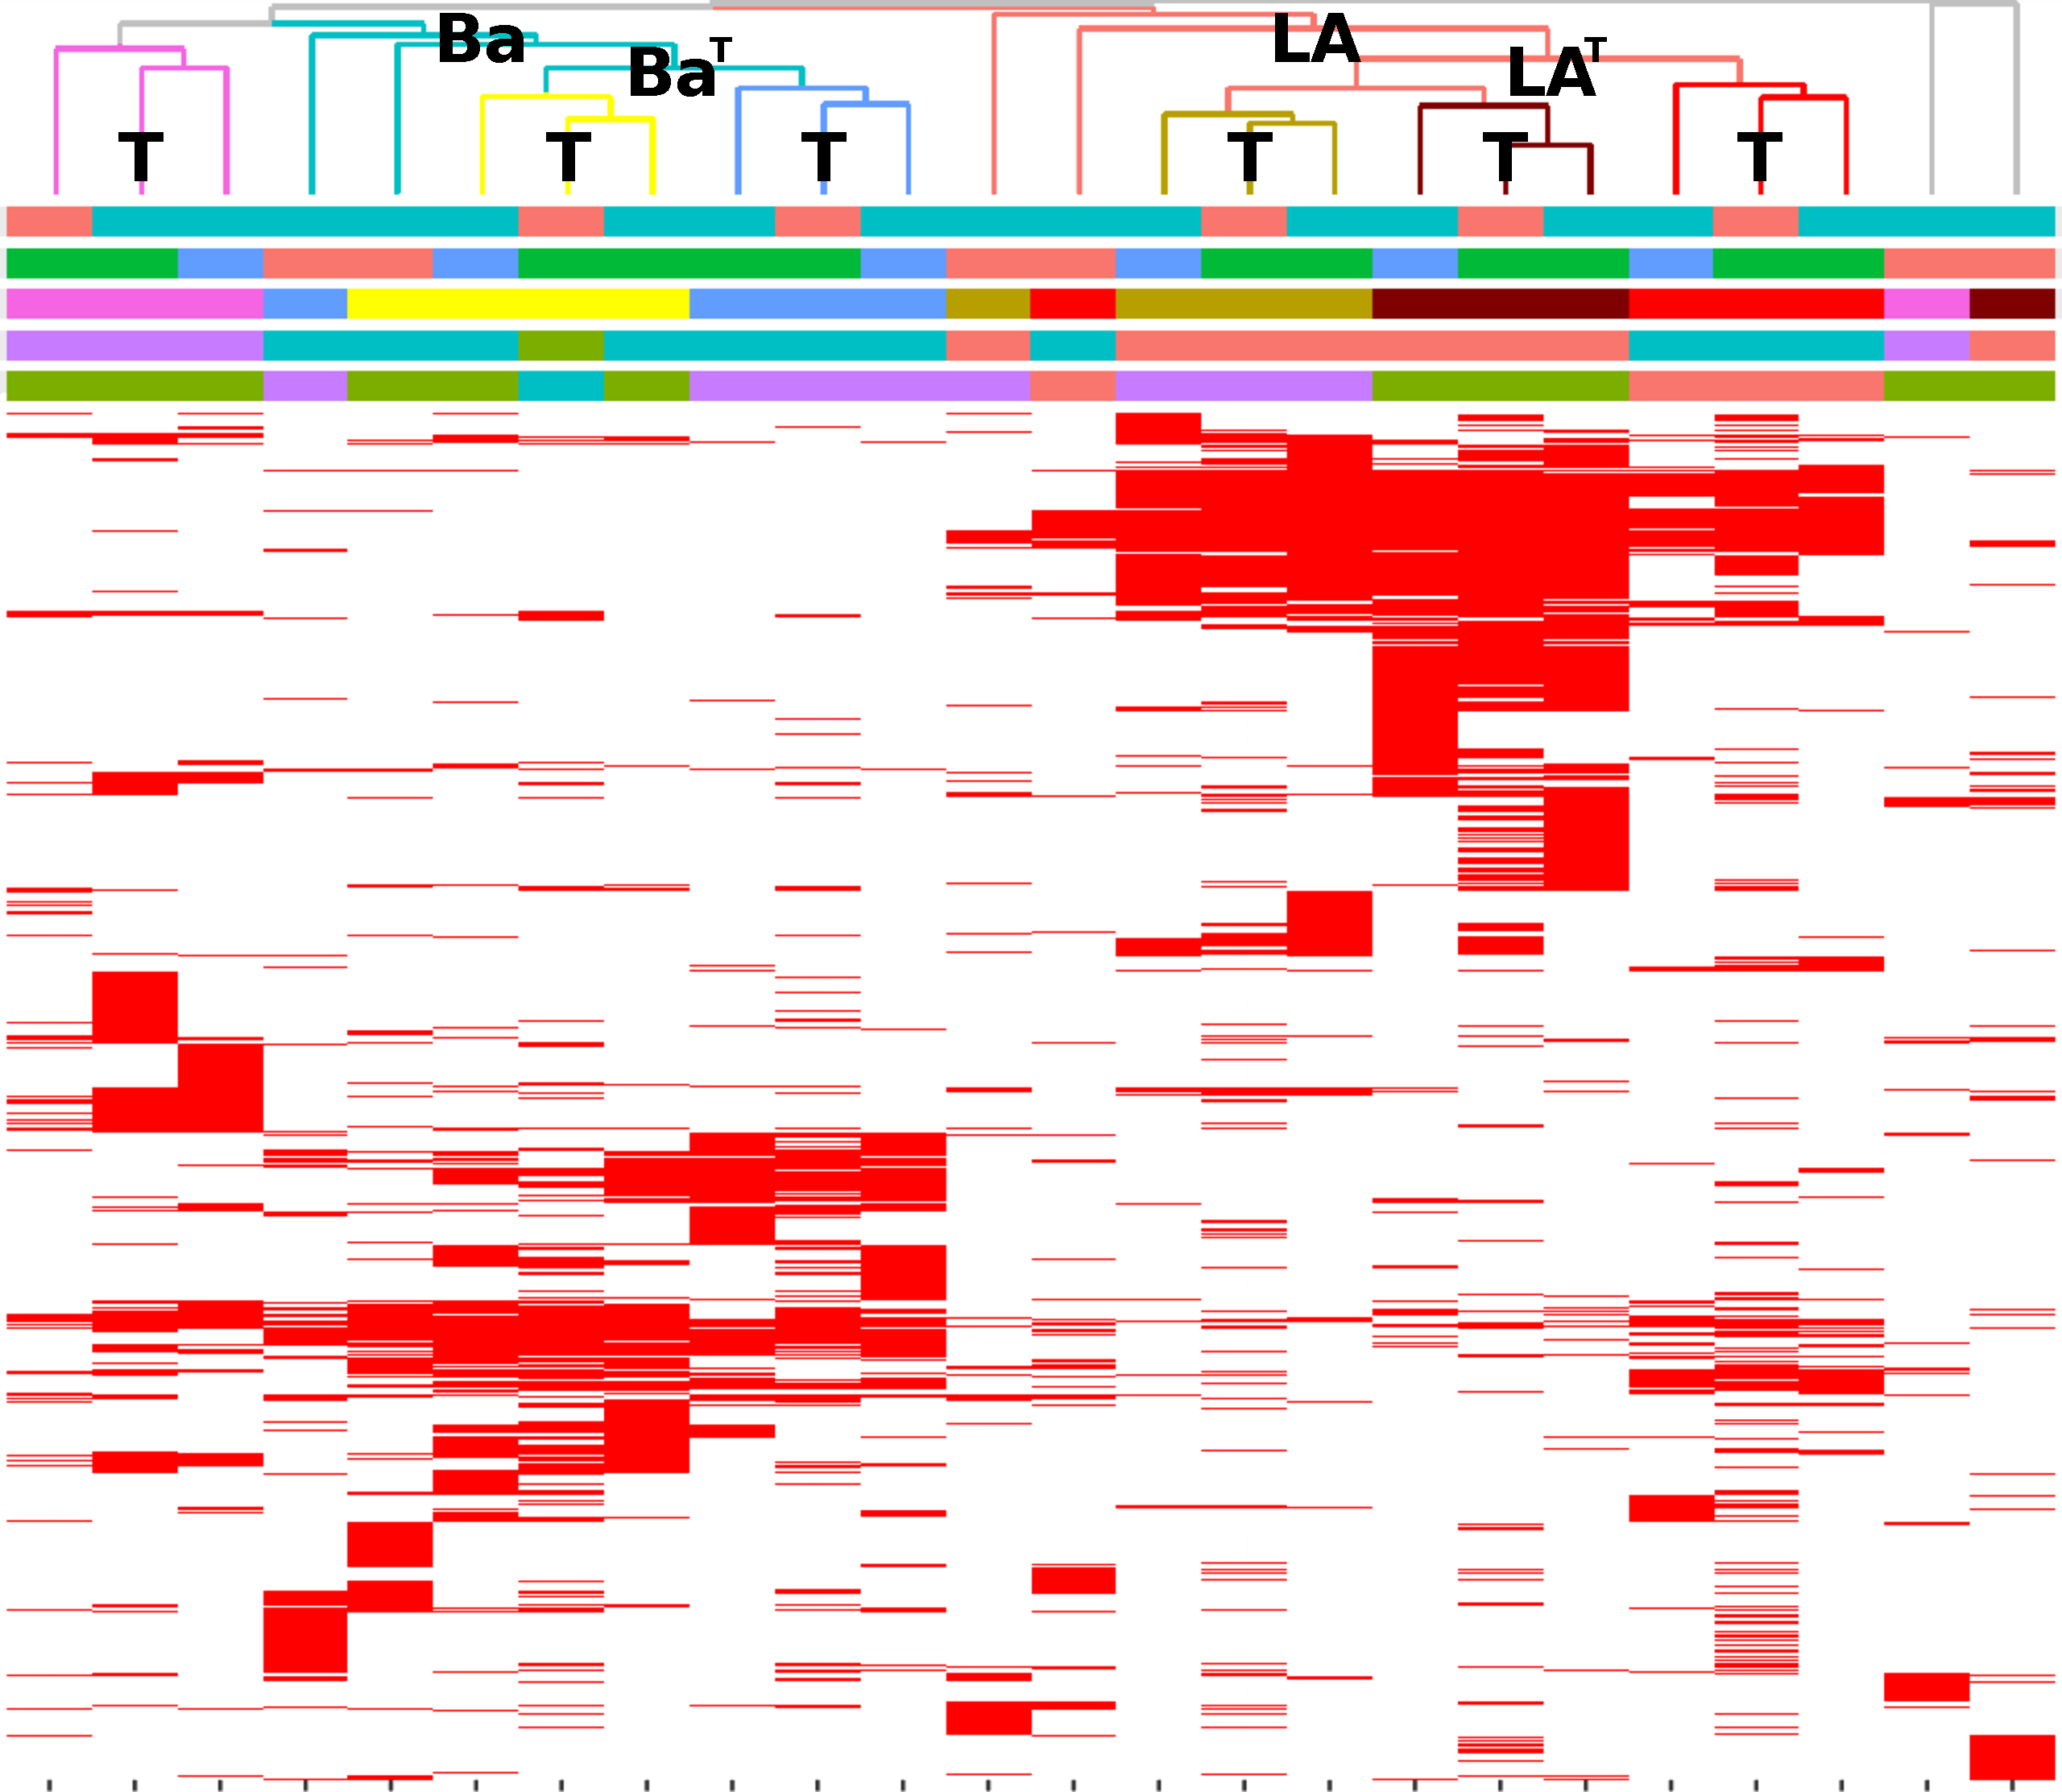
\includegraphics[width=1\linewidth]{images/MIGSA_FIG3} 

}

\caption{Conjuntos de genes enriquecidos por análisis funcional para TCGA. Heatmap: conjuntos de genes en filas, experimentos en columnas; ordenados por distancia Jaccard y enlace promedio. Conjuntos de genes enriquecidos en rojo. Barras de columnas (de arriba abajo): salmón es ``términos enriquecidos por consenso para los conjuntos de datos de Haibe-Kains'', en turquesa datos de TCGA; azul datos de secuenciación de ARN, verde de microarreglos, en salmón de iTRAQ; contraste (comparación entre pares de subtipos); subtipo1 y subtipo2, salmón es Luminal A, turquesa es Basal, púrpura es Her2+, y el verde es Luminal B. Clusters de dendrogramas: Se demarcan para los subtipos Basal (Ba) y Luminal A (LA), para experimentos transcriptómicos de Basal (Ba\(^T\)) y de Luminal A (LA\(^T\)), y para experimentos transcriptómicos específicos por contraste (T).}\label{fig:migsa3}
\end{figure}

\begin{table}[!h]
  \caption{Número de términos enriquecidos compartidos entre plataformas y múltiples ómicas para cada subtipo.}
  \resizebox{\textwidth}{!}{
  \begin{tabular}{lccccccccc}
    \textbf{Subtipo} & \textbf{PTF\textsuperscript{E}} & \textbf{TEP\textsuperscript{E}} & \textbf{TET\textsuperscript{E}} & \textbf{(PTF} & \textbf{(PTF} & \textbf{(TEP} & \textbf{PTF$\cap$} & \textbf{Total} \\
    & & & & \textbf{$\cap$} & \textbf{$\cap$} & \textbf{$\cap$} & \textbf{TEP$\cap$} & \\
    & & & & \textbf{TEP)\textsuperscript{E}} & \textbf{TET)\textsuperscript{E}} & \textbf{TET)\textsuperscript{E}} & \textbf{TET} & \\ \hline
    Basal & 109 & 46 & 21 & 12 & 19  & 0 & 15 & 222 \\
    Luminal B  & 37  & 7  & 25 & 0  & 7   & 0 & 0  & 76  \\
    Her2+      & 42  & 20 & 1  & 0  & 2   & 0 & 0  & 65  \\
    Luminal A  & 234 & 2  & 15 & 3  & 186 & 0 & 14 & 454 \\
    Total      & 422 & 75 & 62 & 15 & 214 & 0 & 29 & 817 \\ \hline
  \end{tabular}
  }
  \label{tab:migsa2}
  \\ \textbf{PTF}: Perfil Transcriptómico Funcional obtenido para cada subtipo a partir de 25 conjuntos de datos basados en microarreglos. \textbf{TEP}: Términos Enriquecidos por Proteómica a partir de datos del TCGA. \textbf{TET}: Términos Enriquecidos por Transcriptómica a partir de datos del TCGA. (X)$^E$ denota los términos en X pero no en las intersecciones de X con los otros conjuntos. (X$\cap$Y)$^E$ denota los términos en X y en Y pero no en las intersecciones de X ó Y con los otros conjuntos.
\end{table}
\hypertarget{exploracion-de-los-resultados-de-tcga-en-conjunto-con-los-ptf}{%
\subsection{Exploración de los resultados de TCGA en conjunto con los PTF}\label{exploracion-de-los-resultados-de-tcga-en-conjunto-con-los-ptf}}

\par

Para cada subtipo, se analizaron los árboles de GO incluyendo los términos enriquecidos por cada categoría presente en las columnas de la Tabla \ref{tab:migsa2}. Como se señaló anteriormente, los términos enriquecidos únicamente en datos proteómicos se encontraron principalmente en los subtipos Basal y Her2+. Por otra parte, para Luminal A y Luminal B los árboles están dominados principalmente por ramas enriquecidas en transcriptómica.

\par

Un hallazgo interesante al analizar los \textbf{TEP} fue la identificación del gen \emph{INPP4B} como un GIE al contrastar los subtipos Basal y Her2+ con los Luminales. En particular, la sobre-expresión de \emph{INPP4B} detectada en los tumores Luminales es consistente con su perfil de expresión reportado por el ``Grupo del Atlas del Genoma del Cáncer'' (Network \& others, 2012) para datos de arrays de proteínas en fase inversa.

\par

Para los sujetos Basales, los GIE tales como \emph{DHRS3}, \emph{LDHB}, \emph{HSD17B8}, \emph{CBR4}, \emph{CYB5A}, y \emph{PHGDH} fueron encontrados en ramas relacionadas con la actividad de la oxidoreductasa. De estos, los GIE de deshidrogenasa, \emph{DHRS3}, \emph{LDHB}, y el \emph{PHGDH} fueron encontrados sobre-expresados en experimentos proteómicos en los cuales el subtipo Basal fue contrastado. Apoyando este hallazgo, la sobre-expresión de la proteína \emph{PHGDH} ha sido previamente relacionada con tumores Basales (Gromova et al., 2015). Además, este gen se ha asociado con la proliferación celular, la migración y los procesos de invasión, y recientemente se ha identificado como un biomarcador inmunohistoquímico de cáncer (Song, Feng, Lu, Lin, \& Dong, 2018).

\par

El análisis de los árboles de Luminal B incluye una rama de \textbf{TEP} relacionada con la secreción hormonal. En esta rama, se encontraron genes tales como \emph{GATA3}, \emph{IRS1}, \emph{BAD}, \emph{SYTL4}, \emph{NDUFAF2}, \emph{GPLD1}, \emph{EGFR}, \emph{FGB}, \emph{FGG}, y \emph{LYN}. En particular, para el contraste proteómico Luminal B vs.~Her2+, \emph{EGFR} se encontró des-regulado para Luminal B, mientras que \emph{GATA3} estaba sobre-expresado, tal como se informa para arrays de proteínas en fase inversa por el ``Grupo del Atlas del Genoma del Cáncer'' (Network \& others, 2012). Otra rama, relacionada con los ribosomas, fue encontrada para Luminal B, en la cual varios genes ribosómicos mitocondriales fueron encontrados como GIE: \emph{MRPL18}, \emph{MRPL28}, \emph{MRPL37}, \emph{MRPL45}, \emph{MRPL48}, \emph{MRPL50}, \emph{MRPL53}, y \emph{MRPL54}; todos ellos fueron encontrados sobre-expresados en Luminal B contrastándolo con Luminal A.

\par

Como se muestra en la Tabla \ref{tab:migsa2}, 29 términos previamente identificados en los \textbf{PTF} de los subtipos de CM también fueron detectados en los respectivos \textbf{TEP} y \textbf{TET}. Entre estos, se encontraron términos que diferencian el subtipo Basal, como el término de FM de unión al distroglicano; y el de PB de regulación positiva de la vía de señalización del receptor de estrógeno intracelular. Para el subtipo Luminal A, se detectó una rama de CC relacionada con el cromosoma condensado, y términos de PB asociados a ciclos celulares mitóticos y meióticos. Veintidós GIE fueron encontrados contribuyendo al enriquecimiento de términos para \textbf{PTF}, \textbf{TEP} y \textbf{TET}. De ellos, 11 fueron identificados para el subtipo Basal (por ejemplo, \emph{AR}, \emph{GATA3}, \emph{FOXA1}, \emph{NFIB}, \emph{AGR2}, \emph{CA12}, y \emph{DSC2}) y 11 para los tumores Luminal A (por ejemplo, \emph{TOP2A}, \emph{CCNB1}, \emph{CDC20}, \emph{UBE2C}, \emph{TTK}, y \emph{KIF2C}). Cabe destacar que todos estos genes se comportaron de acuerdo con las observaciones realizadas por el ``Grupo del Atlas del Genoma del Cáncer'' (Network \& others, 2012).

\hypertarget{conclusiones-1}{%
\section{Conclusiones}\label{conclusiones-1}}

\par

En este capítulo se presentó el paquete R \texttt{MIGSA} para el Análisis Masivo e Integrador de Conjuntos de Genes. Esta herramienta realiza un análisis funcional completo/integrador, masivamente sobre varias matrices de expresión de diferentes repositorios y fuentes ómicas. \texttt{MIGSA} facilita la búsqueda de patrones funcionales -que son denotados por conjuntos de genes y que explican fenotipos particulares- por medio de herramientas exploratorias y gráficas. MIGSA también permite a los usuarios indagar en conjuntos de genes particulares para buscar los genes específicos responsables del enriquecimiento funcional. Las capacidades analíticas y exploratorias de \texttt{MIGSA} como herramienta de análisis funcional masivo, en conjunto con el hecho de que a nuestro entender, es la única herramienta existente que permite la comparación de múltiples experimentos desde un punto de vista funcional, la convierten en un enfoque novedoso.

\par

La utilidad de \texttt{MIGSA} quedó demostrada debido a la caracterización funcional de los subtipos de Cáncer de Mama (CM) definidos por Perou et al.~La aplicación de \texttt{MIGSA} sobre 118 experimentos de microarreglos de CM resultó en la identificación de Perfiles Transcriptómicos Funcionales (\textbf{PTF}) y Genes Importantes de Enriquecimiento (GIE) para cada subtipo. La fiabilidad de nuestros hallazgos fue confirmada usando resultados previamente reportados en la literatura. La identificación de GIE con un comportamiento de expresión consistente a través de conjuntos de datos resulta útil para el descubrimiento de genes provocadores de enfermedades, y por ende, buenos blancos a atacar por drogas.

\par

La capacidad de \texttt{MIGSA} de integrar múltiples conjuntos de datos ómicos se demostró aplicándolo a los datasets de CM del TCGA compuestos tanto de datos transcriptómicos (secuenciación de ARN y microarreglos) como proteómicos (iTRAQ). Los resultados obtenidos se utilizaron para identificar, para cada subtipo, el conjunto de Términos Enriquecidos por Transcriptómica (\textbf{TET}) y de Términos Enriquecidos por Proteómica (\textbf{TEP}). Al integrar y comparar estos resultados con los \textbf{PTF} encontrados previamente, se descubrió una alta consistencia de patrones funcionales entre los términos enriquecidos en datos de TCGA y en los \textbf{PTF}. Dado que \texttt{MIGSA} es una herramienta tan flexible, el procedimiento presentado puede ser replicado tanto en otros subtipos de CM como en otras enfermedades con el fin de explorar perfiles funcionales. El paquete \texttt{MIGSA} se encuentra libremente disponible -bajo una licencia GPLv2- en el repositorio Bioconductor \url{https://bioconductor.org/packages/MIGSA/}, y cuenta con más de 3.000 descargas según las estadísticas del repositorio \url{https://bioconductor.org/packages/stats/bioc/MIGSA/} desde su primera versión, en Marzo de 2017.

\hypertarget{cap:desafios}{%
\chapter{Desafíos que surgieron durante el trabajo de tesis}\label{cap:desafios}}

\hypertarget{eficiencia-computacional-del-algoritmo-mgsz}{%
\section{\texorpdfstring{Eficiencia computacional del algoritmo \texttt{mGSZ}}{Eficiencia computacional del algoritmo mGSZ}}\label{eficiencia-computacional-del-algoritmo-mgsz}}

\par

Como se vio en el Capítulo \protect\hyperlink{cap:ifa}{3}, el método \texttt{mGSZ} resultó ser la mejor alternativa para llevar a cabo el análisis funcional del tipo \emph{Puntuación Funcional de Clase}. La función principal de \texttt{mGSZ}, con sus parámetros por defecto -que sugerimos como resultado del Capítulo \protect\hyperlink{cap:ifa}{3}-, realiza un máximo de 200 permutaciones y filtra solo aquellos conjuntos de genes que presentan menos de cinco genes. En este sentido, llevar a cabo el análisis funcional de \texttt{mGSZ} de un experimento ordinario, por ejemplo, Basal vs.~Luminal A de datos de microarreglos del TCGA sobre Gene Ontology, en una computadora estándar, puede tomar alrededor de 2,46 horas, como mostramos a continuación.

\par

Esta demora del algoritmo, puede resultar despreciable si se desea analizar un único experimento. Sin embargo, como objetivo global del presente trabajo de tesis, se propuso una herramienta de exploración, desde un punto de vista funcional, de grandes cantidades de experimentos. Si extrapolamos linealmente la demora del análisis funcional de un experimento a 118 experimentos (el número de experimentos analizados en el Capítulo \protect\hyperlink{cap:migsa}{4}), estaríamos hablando de una espera de 290,28 horas, es decir, 12,09 días. Dada esta situación, resultó fundamental afrontar este desafío, mediante la optimización del algoritmo original de \texttt{mGSZ}, de manera de disminuir el tiempo de ejecución.

\hypertarget{optimizacion-del-algoritmo-mgsz}{%
\subsection{\texorpdfstring{Optimización del algoritmo \texttt{mGSZ}}{Optimización del algoritmo mGSZ}}\label{optimizacion-del-algoritmo-mgsz}}

\par

Para disminuir el tiempo de ejecución de \texttt{mGSZ}, en primer instancia se debió analizar el código del paquete \texttt{mGSZ} de manera de encontrar porciones de código críticas. Mediante los paquetes \texttt{profvis} y \texttt{microbenchmark} se detectaron tanto aquellas porciones de código de más lenta ejecución, como aquellas que más frecuentemente se ejecutaban. Como resultado de este análisis, se obtuvieron unos pocos fragmentos de código que fueron \textbf{objetivos críticos} a optimizar.

\par

La optimización de estos objetivos críticos se llevo a cabo aplicando diversas estrategias de optimización generales (Cooper \& Torczon, 2011; Wolfe, 1996) como también algunas específicas del lenguaje R (Burns, 2011; Gillespie \& Lovelace, 2016; Wickham, 2014). Esta versión optimizada de la función \texttt{mGSZ} se implementó en el paquete \texttt{MIGSA}, y puede utilizarse, independientemente de \texttt{MIGSA}, llamando a la función \texttt{MIGSAmGSZ}.

\par

Con el fin de evaluar las mejoras en tiempo de ejecución de \texttt{MIGSAmGSZ} con respecto a \texttt{mGSZ}, se analizaron ambas funciones dándoles como entrada los mismos input: la matriz de expresión de microarreglos de ADN de cáncer de mama del TCGA (16.207 genes \(\times\) 237 sujetos), donde se contrastaron los subtipos Basal vs.~Luminal A, analizando los conjuntos de genes del Gene Ontology y KEGG (20.425 conjuntos de genes). El análisis se llevó a cabo utilizando un procesador Intel(R) Xeon(R) E5-2620 v3 @ 2.40GHz (24 núcleos), y 128GB de memoria RAM.

\par

Dicha comparación se puede replicar mediante el siguiente código:
\begin{Shaded}
\begin{Highlighting}[]
\KeywordTok{library}\NormalTok{(}\StringTok{"BiocParallel"}\NormalTok{)}
\KeywordTok{library}\NormalTok{(}\StringTok{"mGSZ"}\NormalTok{)}
\KeywordTok{library}\NormalTok{(}\StringTok{"MIGSA"}\NormalTok{)}
\KeywordTok{library}\NormalTok{(}\StringTok{"MIGSAdata"}\NormalTok{)}

\CommentTok{# Cargamos la matriz de expresión del TCGA}
\KeywordTok{data}\NormalTok{(tcgaMAdata)}
\NormalTok{subtipos <-}\StringTok{ }\NormalTok{tcgaMAdata}\OperatorTok{$}\NormalTok{subtypes}
\NormalTok{expresion <-}\StringTok{ }\NormalTok{tcgaMAdata}\OperatorTok{$}\NormalTok{geneExpr}

\KeywordTok{dim}\NormalTok{(expresion) }\CommentTok{# #genes y #sujetos}
\end{Highlighting}
\end{Shaded}
\begin{verbatim}
[1] 16207   237
\end{verbatim}
\begin{Shaded}
\begin{Highlighting}[]
\KeywordTok{table}\NormalTok{(subtipos) }\CommentTok{# #sujetos de cada subtipo}
\end{Highlighting}
\end{Shaded}
\begin{verbatim}
subtipos
Basal  LumA 
   95   142 
\end{verbatim}
\begin{Shaded}
\begin{Highlighting}[]
\CommentTok{# Cargamos los conjuntos de genes de KEGG y Gene Ontology}
\CommentTok{# utilizando funciones de MIGSA}
\NormalTok{conj_genes <-}\StringTok{ }\KeywordTok{list}\NormalTok{(}
  \DataTypeTok{KEGG =} \KeywordTok{downloadEnrichrGeneSets}\NormalTok{(}\StringTok{"KEGG_2015"}\NormalTok{)[[}\DecValTok{1}\NormalTok{]],}
  \DataTypeTok{BP =} \KeywordTok{loadGo}\NormalTok{(}\StringTok{"BP"}\NormalTok{),}
  \DataTypeTok{CC =} \KeywordTok{loadGo}\NormalTok{(}\StringTok{"CC"}\NormalTok{),}
  \DataTypeTok{MF =} \KeywordTok{loadGo}\NormalTok{(}\StringTok{"MF"}\NormalTok{)}
\NormalTok{)}
\NormalTok{conj_genes <-}\StringTok{ }\KeywordTok{do.call}\NormalTok{(c, }\KeywordTok{lapply}\NormalTok{(conj_genes, MIGSA}\OperatorTok{:::}\NormalTok{asList))}
\end{Highlighting}
\end{Shaded}
\begin{Shaded}
\begin{Highlighting}[]
\CommentTok{# Ejecutamos mGSZ original y medimos su tiempo de ejecución}
\KeywordTok{set.seed}\NormalTok{(}\DecValTok{8818}\NormalTok{)}
\NormalTok{mGSZ_tiempo <-}\StringTok{ }\KeywordTok{system.time}\NormalTok{(\{}
\NormalTok{  mGSZ_res <-}\StringTok{ }\KeywordTok{mGSZ}\NormalTok{(expresion, conj_genes, subtipos)}\OperatorTok{$}\NormalTok{mGSZ}
\NormalTok{\})}
\end{Highlighting}
\end{Shaded}
\begin{Shaded}
\begin{Highlighting}[]
\CommentTok{# Ejecutamos MIGSAmGSZ y medimos su tiempo de ejecución}
\KeywordTok{register}\NormalTok{(}\KeywordTok{SerialParam}\NormalTok{()) }\CommentTok{# linea que aclararemos a continuación}
\KeywordTok{set.seed}\NormalTok{(}\DecValTok{8818}\NormalTok{)}
\NormalTok{MIGSAmGSZ_tiempo <-}\StringTok{ }\KeywordTok{system.time}\NormalTok{(\{}
\NormalTok{  MIGSAmGSZ_res <-}\StringTok{ }\KeywordTok{MIGSAmGSZ}\NormalTok{(expresion, conj_genes, subtipos)}
\NormalTok{\})}
\end{Highlighting}
\end{Shaded}
\begin{Shaded}
\begin{Highlighting}[]
\CommentTok{# Vemos el tiempo total ("elapsed") y calculamos Speedup}
\NormalTok{mGSZ_tiempo <-}\StringTok{ }\NormalTok{mGSZ_tiempo[[}\StringTok{"elapsed"}\NormalTok{]]}
\NormalTok{MIGSAmGSZ_tiempo <-}\StringTok{ }\NormalTok{MIGSAmGSZ_tiempo[[}\StringTok{"elapsed"}\NormalTok{]]}
\KeywordTok{c}\NormalTok{(}
  \DataTypeTok{mGSZ =}\NormalTok{ mGSZ_tiempo }\OperatorTok{/}\StringTok{ }\DecValTok{60} \OperatorTok{/}\StringTok{ }\DecValTok{60}\NormalTok{,            }\CommentTok{# en horas}
  \DataTypeTok{MIGSAmGSZ =}\NormalTok{ MIGSAmGSZ_tiempo }\OperatorTok{/}\StringTok{ }\DecValTok{60} \OperatorTok{/}\StringTok{ }\DecValTok{60}\NormalTok{,  }\CommentTok{# en horas}
  \DataTypeTok{Speedup =}\NormalTok{ mGSZ_tiempo }\OperatorTok{/}\StringTok{ }\NormalTok{MIGSAmGSZ_tiempo}
\NormalTok{)}
\end{Highlighting}
\end{Shaded}
\begin{verbatim}
     mGSZ MIGSAmGSZ   Speedup 
 2.461000  1.553534  1.584130 
\end{verbatim}
Como se observa, la versión optimizada, \texttt{MIGSAmGSZ}, presenta un \emph{speedup} de 1,6X sobre el algoritmo original -de demorar 2,46 horas, la nueva versión pasó a demorar 1,55 horas-.

\par

Por otra parte, la implementación original de \texttt{mGSZ} se ejecuta, exclusivamente, de modo secuencial. En la actualidad, siendo tan fácil el acceso a computadores multi-procesador, el algoritmo \texttt{mGSZ} deja de lado una alternativa muy favorable en cuanto a la eficiencia en el tiempo de ejecución.

\par

Como segunda fase de la reimplementación de \texttt{mGSZ}, detectamos cuáles porciones de código de \texttt{MIGSAmGSZ} podrían ejecutarse en paralelo y otorgarían un \emph{speedup} considerable. Utilizando el paquete \texttt{BiocParallel}, se paralelizaron aquellas rutinas que consideramos pertinentes, y se brindó una sencilla interfaz de paralelismo al usuario. El análisis de la ganancia obtenida, gracias al paralelismo de \texttt{MIGSAmGSZ}, se puede replicar mediante el siguiente código:
\begin{Shaded}
\begin{Highlighting}[]
\CommentTok{# Evaluamos MIGSAmGSZ con 1, 2, 4, 8, 10, 12 y 14 núcleos}
\NormalTok{nucleos <-}\StringTok{ }\KeywordTok{c}\NormalTok{(}\DecValTok{1}\NormalTok{, }\DecValTok{2}\NormalTok{, }\DecValTok{4}\NormalTok{, }\DecValTok{8}\NormalTok{, }\DecValTok{10}\NormalTok{, }\DecValTok{12}\NormalTok{, }\DecValTok{14}\NormalTok{)}
\NormalTok{resultados <-}\StringTok{ }\KeywordTok{lapply}\NormalTok{(nucleos, }\ControlFlowTok{function}\NormalTok{(act_nucl) \{}
  \CommentTok{# Mediante las siguientes 4 líneas de código se le indica}
  \CommentTok{# la cantidad de núcleos en las que debe ejecutarse MIGSAmGSZ.}
  \CommentTok{# El parámetro 'workers' indica la cantidad de núcleos a utilizar.}
  \KeywordTok{register}\NormalTok{(}\KeywordTok{MulticoreParam}\NormalTok{(}
    \DataTypeTok{workers =}\NormalTok{ act_nucl, }\DataTypeTok{threshold =} \StringTok{"DEBUG"}\NormalTok{,}
    \DataTypeTok{progressbar =} \OtherTok{TRUE}
\NormalTok{  ))}

  \KeywordTok{set.seed}\NormalTok{(}\DecValTok{8818}\NormalTok{)}
\NormalTok{  MIGSAmGSZ_tiempo <-}\StringTok{ }\KeywordTok{system.time}\NormalTok{(\{}
\NormalTok{    MIGSAmGSZ_res <-}\StringTok{ }\KeywordTok{MIGSAmGSZ}\NormalTok{(expresion, conj_genes, subtipos)}
\NormalTok{  \})}

  \KeywordTok{return}\NormalTok{(}\KeywordTok{list}\NormalTok{(}\DataTypeTok{tiempo =}\NormalTok{ MIGSAmGSZ_tiempo, }\DataTypeTok{res =}\NormalTok{ MIGSAmGSZ_res))}
\NormalTok{\})}
\end{Highlighting}
\end{Shaded}
\begin{Shaded}
\begin{Highlighting}[]
\CommentTok{# Para cada ejecución conservamos el tiempo total ("elapsed") }
\CommentTok{# y calculamos Speedup y Eficiencia sobre mGSZ}
\NormalTok{tiempos_segs <-}\StringTok{ }\KeywordTok{sapply}\NormalTok{(resultados, }\ControlFlowTok{function}\NormalTok{(act_res) \{}
\NormalTok{  act_res}\OperatorTok{$}\NormalTok{tiempo[[}\StringTok{"elapsed"}\NormalTok{]]}
\NormalTok{\})}
\KeywordTok{names}\NormalTok{(tiempos_segs) <-}\StringTok{ }\NormalTok{nucleos}
\NormalTok{metricas <-}\StringTok{ }\KeywordTok{rbind}\NormalTok{(}
  \StringTok{"Demora (mins)"}\NormalTok{ =}\StringTok{ }\NormalTok{tiempos_segs }\OperatorTok{/}\StringTok{ }\DecValTok{60}\NormalTok{, }\CommentTok{# en minutos}
  \DataTypeTok{Speedup =}\NormalTok{ mGSZ_tiempo }\OperatorTok{/}\StringTok{ }\NormalTok{tiempos_segs,}
  \DataTypeTok{Eficiencia =}\NormalTok{ (mGSZ_tiempo }\OperatorTok{/}\StringTok{ }\NormalTok{tiempos_segs) }\OperatorTok{/}\StringTok{ }\NormalTok{nucleos}
\NormalTok{)}
\KeywordTok{round}\NormalTok{(metricas, }\DecValTok{2}\NormalTok{)}
\end{Highlighting}
\end{Shaded}
\begin{verbatim}
                  1     2     4     8    10    12    14
Demora (mins) 93.21 46.50 24.98 15.63 13.67 14.79 28.43
Speedup        1.58  3.18  5.91  9.45 10.81  9.98  5.19
Eficiencia     1.58  1.59  1.48  1.18  1.08  0.83  0.37
\end{verbatim}
\par

Como puede observarse en la tabla superior, sin importar el número de núcleos en los que se haya corrido \texttt{MIGSAmGSZ}, su rendimiento fue superior al de \texttt{mGSZ}. Ejecutándose en un núcleo muestra un \emph{speedup} de 1,6X, alcanzando un máximo de 10,8X con diez núcleos. Gracias a la optimización desarrollada, es posible obtener en 14 minutos los mismos resultados que se obtenían en 2,46 horas de ejecución con el \texttt{mGSZ} original. Extrapolando a 118 experimentos, pasaríamos de una demora de 12,09 días, a tan solo 27,53 horas.

\par

Como se mencionó previamente, la función optimizada y paralelizada \texttt{MIGSAmGSZ} se encuentra incluída en el paquete \texttt{MIGSA}, y se utiliza siguiendo los mismos parámtros que la versión original \texttt{mGSZ}.

\hypertarget{cap:conclusiones}{%
\chapter{Conclusiones y trabajo futuro}\label{cap:conclusiones}}

\par

En esta tesis se presentó la problemática que presenta el Análisis Funcional (AF) frente a grandes cantidades de bases de datos provenientes de diversas fuentes ómicas. Dicha problemática surge debido a la falta de actualización de las metodologías de AF existentes, en contraste con el rápido avance de las tecnologías de obtención de datos de muestras biológicas. Con el surgimiento de tecnologías para obtener datos biológicos de nuevas fuentes, las técnicas de AF quedan obsoletas u otorgan resultados incorrectos. Por otra parte, al disminuir los costos de obtención de datos, la disponibilidad de grandes cantidades de bases de datos es desaprovechada por las metodologías de AF.

\par

En el Capítulo \protect\hyperlink{cap:af}{1} se introdujo al lector en el concepto del análisis funcional. Para ello, en la Sección \ref{sec:ontologias}, se presentó la noción de \emph{Ontología} en el contexto de la biología. Se detallaron varios grupos conocidos de ontologías, como KEGG, BioCarta, Reactome, MSigDB, y Gene Ontology, donde se mostró cómo se estructura su información en conceptos, categorías, términos o vías metabólicas. Luego, en la Sección \ref{sec:af}, se presentaron las distintas metodologías de AF existentes. Se explicó, a grandes rasgos, la idea subyacente a las metodologías de \emph{Análisis de Sobre-Representación} (ASR) y de \emph{Puntuación Funcional de Clase} (PFC) detallando sus ventajas y limitaciones.

\par

El Capítulo \protect\hyperlink{cap:ngs}{2} presentó diversas fuentes de datos biológicas que la tecnología permite cuantificar y que son objeto de análisis. En la Sección \ref{sec:technols} se profundizó en las tecnologías de Microarreglos de ADN, iTRAQ, y Secuenciación de ARN, ya que permiten obtener matrices de expresión, las cuáles son utilizadas como input del AF. Para cada tecnología se especificó la forma en la que obtienen los valores de expresión, y el tipo de dato que devuelven. Luego, en la Sección \ref{sec:repos}, se comentó sobre los diversos repositorios de libre acceso a bases de datos de expresión, la cantidad de sujetos que presenta cada uno y las ómicas que analizan. Finalmente, se mencionaron las condiciones experimentales que resultaban de interés en estos repositorios, para ser inspeccionadas bajo AF.

\par

En el Capítulo \protect\hyperlink{cap:ifa}{3} se llevó a cabo un comparación exhaustiva de diversos algoritmos pertenecientes a las metodologías tanto de ASR como de PFC, junto con combinaciones de sus parámetros. Se mostró que los resultados del AF pueden variar notablemente dependiendo del método y los parámetros utilizados. Lo cual puede influir negativamente en la interpretación biológica si no se aborda adecuadamente. De este capítulo concluimos que tanto el ASR como la PFC proporcionan resultados complementarios que pueden integrarse para obtener una visión biológica más amplia del experimento en estudio. Por ende, presentamos un pipeline de Análisis Funcional Integrador, \texttt{IFA}, que realiza análisis simultáneos de ASR y PFC, proporcionando un marco completo y unificado de AF. Finalmente, se evaluó desde el punto de vista de la biología, los resultados que obtiene este pipeline \texttt{IFA}, lo cual demostró su capacidad de detección de funciones biológicas adecuadas para el fenómeno bajo estudio, además de presentar resultados concordantes entre diversos experimentos.

\par

En el Capítulo \protect\hyperlink{cap:migsa}{4} se presentó el paquete R desarrollado para la presente tesis, \texttt{MIGSA}. Esta herramienta permite realizar un AF completo, integrador, y masivo sobre grandes cantidades de bases de datos. \texttt{MIGSA} posibilita detectar genes y patrones funcionales biológicos, por medio de herramientas exploratorias y gráficas, que caracterizan poblaciones, fenotipos, o grupos de interés. La utilidad de \texttt{MIGSA} quedó demostrada debido a la caracterización funcional de los subtipos de cáncer de mama, donde se logró definir un perfil funcional para cada subtipo. \texttt{MIGSA} efectivamente permitió integrar múltiples bases de datos, y múltiples fuentes de datos (ómicas).

\par

Finalmente, en el Capítulo \protect\hyperlink{cap:desafios}{5} se introdujeron aquellos desafíos que surgieron durante el transcurso de la investigación de la presente tesis, pero que no estaban relacionados directamente con el objetivo bajo estudio. Al notar la lentitud del algoritmo de PFC utilizado por el pipeline \texttt{IFA} y el paquete \texttt{MIGSA}, el desafío principal consistió en disminuir su tiempo de ejecución. En este sentido, luego de un extenso trabajo de optimización y paralelización del algoritmo, se logró un notable \emph{speedup} de 10,8X en el mejor de los casos.

\par

Como propuesta de \textbf{trabajo a futuro}, se desprenden dos líneas de estudio a contemplar. Por una parte, como se mencionó en la Sección \ref{sec:voom}, se debió adaptar el algoritmo \texttt{mGSZ} para que resultara adecuado para analizar datos provenientes de secuenciación de ARN. Para esta adaptación se propuso utilizar la metodología \texttt{voom}, la cuál modela este tipo de datos mediante mínimos cuadrados generalizados (Law et al., 2014). Sin embargo, resulta necesario llevar a cabo una comparación y evaluación extensiva de otras propuestas de manejo de datos de secuenciación de ARN frecuentemente mencionadas por la comunidad científica, entre ellas, \texttt{edgeR} (Robinson, McCarthy, \& Smyth, 2010) y \texttt{DESeq2} (Love, Huber, \& Anders, 2014).

\par

Por otra parte, el paquete \texttt{MIGSA} presenta varios aspectos que pueden ser extendidos, y de los cuales creemos que continuar su desarrollo resultará en notables beneficios para la comunidad científica. Por una parte, con el continuo avance de las tecnologías de obtención de datos ómicos, resulta fundamental actualizar constantemente la herramienta \texttt{MIGSA} de manera que permita el análisis de tipos de datos con diversos supuestos estadísticos subyacentes, como ejemplo de esto, un desafío pendiente es lograr analizar datos de transcriptos de genes. Como segundo objetivo, resultaría interesante poder extender \texttt{MIGSA} al análisis de nuevos diseños experimentales. En la actualidad, \texttt{MIGSA} permite utilizar cualquier diseño experimental, sin embargo no se ha evaluado la correctitud estadística de utilizar otros diseños -aparte de caso vs.~control- en este tipo de AF. Como tercer objetivo a futuro, proponemos idear e implementar nuevas técnicas de exploración y visualización de los resultados de \texttt{MIGSA}, esto permitirá nuevas estrategias para inspeccionar resultados y generar nuevas hipótesis. Finalmente, creemos que extender \texttt{MIGSA} de manera que incluya una interfaz gráfica de usuario, aumentará el público de la herramienta, incorporando aquellos usuarios no tan acostumbrados al ambiente de la programación. Mediante la librería de R \texttt{shiny}, crear interfaces que corren código R resulta sencillo (Rodriguez, Vargas, \& Fernández, 2018) y extremadamente útil.

\hypertarget{bibliografia}{%
\chapter*{Bibliografía}\label{bibliografia}}
\addcontentsline{toc}{chapter}{Bibliografía}

\hypertarget{refs}{}
\leavevmode\hypertarget{ref-ashburner2000gene}{}%
Ashburner, M., Ball, C. A., Blake, J. A., Botstein, D., Butler, H., Cherry, J. M., \ldots{} others. (2000). Gene ontology: Tool for the unification of biology. \emph{Nature Genetics}, \emph{25}(1), 25.

\leavevmode\hypertarget{ref-atchley2008clinical}{}%
Atchley, D. P., Albarracin, C. T., Lopez, A., Valero, V., Amos, C. I., Gonzalez-Angulo, A. M., \ldots{} Arun, B. K. (2008). Clinical and pathologic characteristics of patients with brca-positive and brca-negative breast cancer. \emph{Journal of Clinical Oncology}, \emph{26}(26), 4282--4288.

\leavevmode\hypertarget{ref-aure2017integrative}{}%
Aure, M. R., Vitelli, V., Jernström, S., Kumar, S., Krohn, M., Due, E. U., \ldots{} others. (2017). Integrative clustering reveals a novel split in the luminal a subtype of breast cancer with impact on outcome. \emph{Breast Cancer Research}, \emph{19}(1), 44.

\leavevmode\hypertarget{ref-barrett2012ncbi}{}%
Barrett, T., Wilhite, S. E., Ledoux, P., Evangelista, C., Kim, I. F., Tomashevsky, M., \ldots{} others. (2012). NCBI geo: Archive for functional genomics data sets---update. \emph{Nucleic Acids Research}, \emph{41}(D1), D991--D995.

\leavevmode\hypertarget{ref-bastien2012pam50}{}%
Bastien, R. R., Rodrı'guez-Lescure, Á., Ebbert, M. T., Prat, A., Munárriz, B., Rowe, L., \ldots{} others. (2012). PAM50 breast cancer subtyping by rt-qPCR and concordance with standard clinical molecular markers. \emph{BMC Medical Genomics}, \emph{5}(1), 1.

\leavevmode\hypertarget{ref-berkeley2004linear}{}%
Berkeley, C. (2004). Linear models and empirical bayes methods for assessing differential expression in microarray experiments. \emph{E-Book Available at Http://Www. Bepress. Com/Sagmb/Vol3/Iss1/Art3.{[}PubMed{]}}.

\leavevmode\hypertarget{ref-bittner2005expression}{}%
Bittner, M. (2005). Expression project for oncology (expo). \emph{National Center for Biotechnology Information. Available at: Http://Www. Ncbi. Nlm. Nih. Gov/Geo}.

\leavevmode\hypertarget{ref-bonnefoi2007retracted}{}%
Bonnefoi, H., Potti, A., Delorenzi, M., Mauriac, L., Campone, M., Tubiana-Hulin, M., \ldots{} others. (2007). RETRACTED: Validation of gene signatures that predict the response of breast cancer to neoadjuvant chemotherapy: A substudy of the eortc 10994/big 00-01 clinical trial. Elsevier.

\leavevmode\hypertarget{ref-bos2009genes}{}%
Bos, P. D., Zhang, X. H.-F., Nadal, C., Shu, W., Gomis, R. R., Nguyen, D. X., \ldots{} others. (2009). Genes that mediate breast cancer metastasis to the brain. \emph{Nature}, \emph{459}(7249), 1005.

\leavevmode\hypertarget{ref-burns2011r}{}%
Burns, P. (2011). \emph{The r inferno}. Lulu. com.

\leavevmode\hypertarget{ref-cantor2001bach1}{}%
Cantor, S. B., Bell, D. W., Ganesan, S., Kass, E. M., Drapkin, R., Grossman, S., \ldots{} others. (2001). BACH1, a novel helicase-like protein, interacts directly with brca1 and contributes to its dna repair function. \emph{Cell}, \emph{105}(1), 149--160.

\leavevmode\hypertarget{ref-canuel2014translational}{}%
Canuel, V., Rance, B., Avillach, P., Degoulet, P., \& Burgun, A. (2014). Translational research platforms integrating clinical and omics data: A review of publicly available solutions. \emph{Briefings in Bioinformatics}, \emph{16}(2), 280--290.

\leavevmode\hypertarget{ref-carlson2013org}{}%
Carlson, M., Falcon, S., Pages, H., \& Li, N. (2013). Org. Hs. Eg. Db: Genome wide annotation for human. R package version.

\leavevmode\hypertarget{ref-cheang2009ki67}{}%
Cheang, M. C., Chia, S. K., Voduc, D., Gao, D., Leung, S., Snider, J., \ldots{} others. (2009). Ki67 index, her2 status, and prognosis of patients with luminal b breast cancer. \emph{JNCI: Journal of the National Cancer Institute}, \emph{101}(10), 736--750.

\leavevmode\hypertarget{ref-chen2013promise}{}%
Chen, R., \& Snyder, M. (2013). Promise of personalized omics to precision medicine. \emph{Wiley Interdisciplinary Reviews: Systems Biology and Medicine}, \emph{5}(1), 73--82.

\leavevmode\hypertarget{ref-chin2006genomic}{}%
Chin, K., DeVries, S., Fridlyand, J., Spellman, P. T., Roydasgupta, R., Kuo, W.-L., \ldots{} others. (2006). Genomic and transcriptional aberrations linked to breast cancer pathophysiologies. \emph{Cancer Cell}, \emph{10}(6), 529--541.

\leavevmode\hypertarget{ref-cleveland2001data}{}%
Cleveland, W. S. (2001). Data science: An action plan for expanding the technical areas of the field of statistics. \emph{International Statistical Review}, \emph{69}(1), 21--26.

\leavevmode\hypertarget{ref-gene2016expansion}{}%
Consortium, G. O. (2016). Expansion of the gene ontology knowledgebase and resources. \emph{Nucleic Acids Research}, \emph{45}(D1), D331--D338.

\leavevmode\hypertarget{ref-cooper2011engineering}{}%
Cooper, K., \& Torczon, L. (2011). \emph{Engineering a compiler}. Elsevier.

\leavevmode\hypertarget{ref-creighton2018pan}{}%
Creighton, C. J., Chen, F., Zhang, Y., Gibbons, D. L., Deneen, B., Kwiatkowski, D., \& Ittmann, M. (2018). Pan-cancer molecular classes transcending tumor lineage across 32 cancer types, multiple data platforms, and over 10,000 cases. \emph{Clinical Cancer Research}, clincanres--3378.

\leavevmode\hypertarget{ref-curtis2012genomic}{}%
Curtis, C., Shah, S. P., Chin, S.-F., Turashvili, G., Rueda, O. M., Dunning, M. J., \ldots{} others. (2012). The genomic and transcriptomic architecture of 2,000 breast tumours reveals novel subgroups. \emph{Nature}, \emph{486}(7403), 346.

\leavevmode\hypertarget{ref-dai2015breast}{}%
Dai, X., Li, T., Bai, Z., Yang, Y., Liu, X., Zhan, J., \& Shi, B. (2015). Breast cancer intrinsic subtype classification, clinical use and future trends. \emph{American Journal of Cancer Research}, \emph{5}(10), 2929.

\leavevmode\hypertarget{ref-davis2014comparative}{}%
Davis, A. P., Grondin, C. J., Lennon-Hopkins, K., Saraceni-Richards, C., Sciaky, D., King, B. L., \ldots{} Mattingly, C. J. (2014). The comparative toxicogenomics database's 10th year anniversary: Update 2015. \emph{Nucleic Acids Research}, gku935.

\leavevmode\hypertarget{ref-dedeurwaerder2011dna}{}%
Dedeurwaerder, S., Desmedt, C., Calonne, E., Singhal, S. K., Haibe-Kains, B., Defrance, M., \ldots{} others. (2011). DNA methylation profiling reveals a predominant immune component in breast cancers. \emph{EMBO Molecular Medicine}, \emph{3}(12), 726--741.

\leavevmode\hypertarget{ref-edelman2006analysis}{}%
Edelman, E., Porrello, A., Guinney, J., Balakumaran, B., Bild, A., Febbo, P. G., \& Mukherjee, S. (2006). Analysis of sample set enrichment scores: Assaying the enrichment of sets of genes for individual samples in genome-wide expression profiles. \emph{Bioinformatics}, \emph{22}(14), e108--e116.

\leavevmode\hypertarget{ref-ein2005outcome}{}%
Ein-Dor, L., Kela, I., Getz, G., Givol, D., \& Domany, E. (2005). Outcome signature genes in breast cancer: Is there a unique set? \emph{Bioinformatics}, \emph{21}(2), 171--178.

\leavevmode\hypertarget{ref-ein2006thousands}{}%
Ein-Dor, L., Zuk, O., \& Domany, E. (2006). Thousands of samples are needed to generate a robust gene list for predicting outcome in cancer. \emph{Proceedings of the National Academy of Sciences}, \emph{103}(15), 5923--5928.

\leavevmode\hypertarget{ref-falcon2006using}{}%
Falcon, S., \& Gentleman, R. (2006). Using gostats to test gene lists for go term association. \emph{Bioinformatics}, \emph{23}(2), 257--258.

\leavevmode\hypertarget{ref-falcon2007using}{}%
Falcon, S., \& Gentleman, R. (2007). Using gostats to test gene lists for go term association. \emph{Bioinformatics}, \emph{23}(2), 257--258.

\leavevmode\hypertarget{ref-fang2014thednet}{}%
Fang, H., \& Gough, J. (2014). Thednet'approach promotes emerging research on cancer patient survival. \emph{Genome Medicine}, \emph{6}(8), 64.

\leavevmode\hypertarget{ref-farmer2005identification}{}%
Farmer, P., Bonnefoi, H., Becette, V., Tubiana-Hulin, M., Fumoleau, P., Larsimont, D., \ldots{} others. (2005). Identification of molecular apocrine breast tumours by microarray analysis. \emph{Breast Cancer Research}, \emph{7}(2), P2--11.

\leavevmode\hypertarget{ref-fernandez2018current}{}%
Fernandez, E. A., \& Casares, F. M. (2018). Current challenges for big omics data analytics and precision medicine. \emph{Med Sci Tech}, \emph{59}, 1--3.

\leavevmode\hypertarget{ref-fernandez2007genomica}{}%
Fernández, E., Alvarez, M., Podhajcer, O., \& Stolovitzky, G. (2007). Genomica funcional: En busca de la función de los genes. \emph{National Academy of Science, Argentine}, \emph{13}, 63--76.

\leavevmode\hypertarget{ref-fresno2013rdavidwebservice}{}%
Fresno, C., \& Fernández, E. A. (2013). RDAVIDWebService: A versatile r interface to david. \emph{Bioinformatics}, \emph{29}(21), 2810--2811.

\leavevmode\hypertarget{ref-fresno2016novel}{}%
Fresno, C., González, G. A., Merino, G. A., Flesia, A. G., Podhajcer, O. L., Llera, A. S., \& Fernández, E. A. (2016). A novel non-parametric method for uncertainty evaluation of correlation-based molecular signatures: Its application on pam50 algorithm. \emph{Bioinformatics}, \emph{33}(5), 693--700.

\leavevmode\hypertarget{ref-fresnocontrol}{}%
Fresno, C., González, G. A., Merino, G. A., Rodriguez, J. C., Balzarini, M. G., \& Fernández, E. A. (2014). Control de calidad de microarreglos de adn mediante descomposición anova-pca/pls. \emph{XIX Reunión Científica Del Grupo Argentino de Biometría}.

\leavevmode\hypertarget{ref-fresno2012multi}{}%
Fresno, C., Llera, A. S., Girotti, M. R., Valacco, M. P., López, J. A., Podhajcer, O. L., \ldots{} Fernández, E. A. (2012). The multi-reference contrast method: Facilitating set enrichment analysis. \emph{Computers in Biology and Medicine}, \emph{42}(2), 188--194.

\leavevmode\hypertarget{ref-gendoo2015genefu}{}%
Gendoo, D. M., Ratanasirigulchai, N., Schröder, M. S., Paré, L., Parker, J. S., Prat, A., \& Haibe-Kains, B. (2015). Genefu: An r/bioconductor package for computation of gene expression-based signatures in breast cancer. \emph{Bioinformatics}, \emph{32}(7), 1097--1099.

\leavevmode\hypertarget{ref-gillespie2016efficient}{}%
Gillespie, C., \& Lovelace, R. (2016). \emph{Efficient r programming: A practical guide to smarter programming}. " O'Reilly Media, Inc.".

\leavevmode\hypertarget{ref-goeman2007analyzing}{}%
Goeman, J. J., \& Bühlmann, P. (2007). Analyzing gene expression data in terms of gene sets: Methodological issues. \emph{Bioinformatics}, \emph{23}(8), 980--987.

\leavevmode\hypertarget{ref-goldhirsch2013personalizing}{}%
Goldhirsch, A., Winer, E. P., Coates, A., Gelber, R., Piccart-Gebhart, M., Thürlimann, B., \ldots{} others. (2013). Personalizing the treatment of women with early breast cancer: Highlights of the st gallen international expert consensus on the primary therapy of early breast cancer 2013. \emph{Annals of Oncology}, \emph{24}(9), 2206--2223.

\leavevmode\hypertarget{ref-grasso2012mutational}{}%
Grasso, C. S., Wu, Y.-M., Robinson, D. R., Cao, X., Dhanasekaran, S. M., Khan, A. P., \ldots{} others. (2012). The mutational landscape of lethal castration-resistant prostate cancer. \emph{Nature}, \emph{487}(7406), 239.

\leavevmode\hypertarget{ref-gromova2015high}{}%
Gromova, I., Gromov, P., Honma, N., Kumar, S., Rimm, D., Talman, M.-L. M., \ldots{} Moreira, J. (2015). High level phgdh expression in breast is predominantly associated with keratin 5-positive cell lineage independently of malignancy. \emph{Molecular Oncology}, \emph{9}(8), 1636--1654.

\leavevmode\hypertarget{ref-guen2017emt}{}%
Guen, V. J., Chavarria, T. E., Kröger, C., Ye, X., Weinberg, R. A., \& Lees, J. A. (2017). EMT programs promote basal mammary stem cell and tumor-initiating cell stemness by inducing primary ciliogenesis and hedgehog signaling. \emph{Proceedings of the National Academy of Sciences}, 201711534.

\leavevmode\hypertarget{ref-haibe2012three}{}%
Haibe-Kains, B., Desmedt, C., Loi, S., Culhane, A. C., Bontempi, G., Quackenbush, J., \& Sotiriou, C. (2012). A three-gene model to robustly identify breast cancer molecular subtypes. \emph{Journal of the National Cancer Institute}, \emph{104}(4), 311--325.

\leavevmode\hypertarget{ref-hanahan2000hallmarks}{}%
Hanahan, D., \& Weinberg, R. A. (2000). The hallmarks of cancer. \emph{Cell}, \emph{100}(1), 57--70.

\leavevmode\hypertarget{ref-hess2006pharmacogenomic}{}%
Hess, K. R., Anderson, K., Symmans, W. F., Valero, V., Ibrahim, N., Mejia, J. A., \ldots{} others. (2006). Pharmacogenomic predictor of sensitivity to preoperative chemotherapy with paclitaxel and fluorouracil, doxorubicin, and cyclophosphamide in breast cancer. \emph{Journal of Clinical Oncology}, \emph{24}(26), 4236--4244.

\leavevmode\hypertarget{ref-hoadley2014multiplatform}{}%
Hoadley, K. A., Yau, C., Wolf, D. M., Cherniack, A. D., Tamborero, D., Ng, S., \ldots{} others. (2014). Multiplatform analysis of 12 cancer types reveals molecular classification within and across tissues of origin. \emph{Cell}, \emph{158}(4), 929--944.

\leavevmode\hypertarget{ref-huang2008bioinformatics}{}%
Huang, D. W., Sherman, B. T., \& Lempicki, R. A. (2008a). Bioinformatics enrichment tools: Paths toward the comprehensive functional analysis of large gene lists. \emph{Nucleic Acids Research}, \emph{37}(1), 1--13.

\leavevmode\hypertarget{ref-huang2008systematic}{}%
Huang, D. W., Sherman, B. T., \& Lempicki, R. A. (2008b). Systematic and integrative analysis of large gene lists using david bioinformatics resources. \emph{Nature Protocols}, \emph{4}(1), 44.

\leavevmode\hypertarget{ref-huang2009systematic}{}%
Huang, D. W., Sherman, B. T., \& Lempicki, R. A. (2009). Systematic and integrative analysis of large gene lists using david bioinformatics resources. \emph{Nature Protocols}, \emph{4}(1), 44--57.

\leavevmode\hypertarget{ref-joshi2005reactome}{}%
Joshi-Tope, G., Gillespie, M., Vastrik, I., D'Eustachio, P., Schmidt, E., Bono, B. de, \ldots{} others. (2005). Reactome: A knowledgebase of biological pathways. \emph{Nucleic Acids Research}, \emph{33}(suppl\_1), D428--D432.

\leavevmode\hypertarget{ref-kanehisa2000kegg}{}%
Kanehisa, M., \& Goto, S. (2000). KEGG: Kyoto encyclopedia of genes and genomes. \emph{Nucleic Acids Research}, \emph{28}(1), 27--30.

\leavevmode\hypertarget{ref-kedaigle2018turning}{}%
Kedaigle, A., \& Fraenkel, E. (2018). Turning omics data into therapeutic insights. \emph{Current Opinion in Pharmacology}, \emph{42}, 95--101.

\leavevmode\hypertarget{ref-khatri2012ten}{}%
Khatri, P., Sirota, M., \& Butte, A. J. (2012). Ten years of pathway analysis: Current approaches and outstanding challenges. \emph{PLoS Computational Biology}, \emph{8}(2), e1002375.

\leavevmode\hypertarget{ref-kolesnikov2014arrayexpress}{}%
Kolesnikov, N., Hastings, E., Keays, M., Melnichuk, O., Tang, Y. A., Williams, E., \ldots{} others. (2014). ArrayExpress update---simplifying data submissions. \emph{Nucleic Acids Research}, \emph{43}(D1), D1113--D1116.

\leavevmode\hypertarget{ref-korkola2007identification}{}%
Korkola, J. E., Blaveri, E., DeVries, S., Moore, D. H., Hwang, E. S., Chen, Y.-Y., \ldots{} Waldman, F. M. (2007). Identification of a robust gene signature that predicts breast cancer outcome in independent data sets. \emph{BMC Cancer}, \emph{7}(1), 61.

\leavevmode\hypertarget{ref-kuleshov2016enrichr}{}%
Kuleshov, M. V., Jones, M. R., Rouillard, A. D., Fernandez, N. F., Duan, Q., Wang, Z., \ldots{} others. (2016). Enrichr: A comprehensive gene set enrichment analysis web server 2016 update. \emph{Nucleic Acids Research}, \emph{44}(W1), W90--W97.

\leavevmode\hypertarget{ref-kwa2017clinical}{}%
Kwa, M., Makris, A., \& Esteva, F. J. (2017). Clinical utility of gene-expression signatures in early stage breast cancer. \emph{Nature Reviews Clinical Oncology}, \emph{14}(10), 595.

\leavevmode\hypertarget{ref-law2014voom}{}%
Law, C. W., Chen, Y., Shi, W., \& Smyth, G. K. (2014). Voom: Precision weights unlock linear model analysis tools for rna-seq read counts. \emph{Genome Biology}, \emph{15}(2), R29.

\leavevmode\hypertarget{ref-li2010minimising}{}%
Li, Q., Eklund, A. C., Juul, N., Haibe-Kains, B., Workman, C. T., Richardson, A. L., \ldots{} Swanton, C. (2010). Minimising immunohistochemical false negative er classification using a complementary 23 gene expression signature of er status. \emph{PloS One}, \emph{5}(12), e15031.

\leavevmode\hypertarget{ref-liberzon2011molecular}{}%
Liberzon, A., Subramanian, A., Pinchback, R., Thorvaldsdóttir, H., Tamayo, P., \& Mesirov, J. P. (2011). Molecular signatures database (msigdb) 3.0. \emph{Bioinformatics}, \emph{27}(12), 1739--1740.

\leavevmode\hypertarget{ref-liedtke2008response}{}%
Liedtke, C., Mazouni, C., Hess, K. R., André, F., Tordai, A., Mejia, J. A., \ldots{} others. (2008). Response to neoadjuvant therapy and long-term survival in patients with triple-negative breast cancer. \emph{Journal of Clinical Oncology}, \emph{26}(8), 1275--1281.

\leavevmode\hypertarget{ref-liu2016integrative}{}%
Liu, B., Shen, X., \& Pan, W. (2016). Integrative and regularized principal component analysis of multiple sources of data. \emph{Statistics in Medicine}, \emph{35}(13), 2235--2250.

\leavevmode\hypertarget{ref-llera2015translational}{}%
Llera, A. S., Podhajcer, O. L., Breitenbach, M., Santini, L., Muller, B., Daneri Navarro, A., \ldots{} others. (2015). Translational cancer research comes of age in latin america. In \emph{American sci transl med} (Vol. 7, p. 319). American Association for the Advancement of Science.

\leavevmode\hypertarget{ref-love2014moderated}{}%
Love, M. I., Huber, W., \& Anders, S. (2014). Moderated estimation of fold change and dispersion for rna-seq data with deseq2. \emph{Genome Biology}, \emph{15}(12), 550.

\leavevmode\hypertarget{ref-lu2008predicting}{}%
Lu, X., Lu, X., Wang, Z. C., Iglehart, J. D., Zhang, X., \& Richardson, A. L. (2008). Predicting features of breast cancer with gene expression patterns. \emph{Breast Cancer Research and Treatment}, \emph{108}(2), 191.

\leavevmode\hypertarget{ref-manoli2006group}{}%
Manoli, T., Gretz, N., Gröne, H.-J., Kenzelmann, M., Eils, R., \& Brors, B. (2006). Group testing for pathway analysis improves comparability of different microarray datasets. \emph{Bioinformatics}, \emph{22}(20), 2500--2506.

\leavevmode\hypertarget{ref-mccarthy2009testing}{}%
McCarthy, D. J., \& Smyth, G. K. (2009). Testing significance relative to a fold-change threshold is a treat. \emph{Bioinformatics}, \emph{25}(6), 765--771.

\leavevmode\hypertarget{ref-meng2014multivariate}{}%
Meng, C., Kuster, B., Culhane, A. C., \& Gholami, A. M. (2014). A multivariate approach to the integration of multi-omics datasets. \emph{BMC Bioinformatics}, \emph{15}(1), 162.

\leavevmode\hypertarget{ref-metzger2011genomic}{}%
Metzger Filho, O., Ignatiadis, M., \& Sotiriou, C. (2011). Genomic grade index: An important tool for assessing breast cancer tumor grade and prognosis. \emph{Critical Reviews in Oncology/Hematology}, \emph{77}(1), 20--29.

\leavevmode\hypertarget{ref-miller2005expression}{}%
Miller, L. D., Smeds, J., George, J., Vega, V. B., Vergara, L., Ploner, A., \ldots{} others. (2005). An expression signature for p53 status in human breast cancer predicts mutation status, transcriptional effects, and patient survival. \emph{Proceedings of the National Academy of Sciences}, \emph{102}(38), 13550--13555.

\leavevmode\hypertarget{ref-minn2007lung}{}%
Minn, A. J., Gupta, G. P., Padua, D., Bos, P., Nguyen, D. X., Nuyten, D., \ldots{} others. (2007). Lung metastasis genes couple breast tumor size and metastatic spread. \emph{Proceedings of the National Academy of Sciences}, \emph{104}(16), 6740--6745.

\leavevmode\hypertarget{ref-minn2005genes}{}%
Minn, A. J., Gupta, G. P., Siegel, P. M., Bos, P. D., Shu, W., Giri, D. D., \ldots{} Massagué, J. (2005). Genes that mediate breast cancer metastasis to lung. \emph{Nature}, \emph{436}(7050), 518.

\leavevmode\hypertarget{ref-mishra2014gene}{}%
Mishra, P., Törönen, P., Leino, Y., \& Holm, L. (2014). Gene set analysis: Limitations in popular existing methods and proposed improvements. \emph{Bioinformatics}, \emph{30}(19), 2747--2756.

\leavevmode\hypertarget{ref-natrajan2010integrative}{}%
Natrajan, R., Weigelt, B., Mackay, A., Geyer, F. C., Grigoriadis, A., Tan, D. S., \ldots{} others. (2010). An integrative genomic and transcriptomic analysis reveals molecular pathways and networks regulated by copy number aberrations in basal-like, her2 and luminal cancers. \emph{Breast Cancer Research and Treatment}, \emph{121}(3), 575--589.

\leavevmode\hypertarget{ref-cancer2012comprehensive}{}%
Network, C. G. A., \& others. (2012). Comprehensive molecular portraits of human breast tumours. \emph{Nature}, \emph{490}(7418), 61.

\leavevmode\hypertarget{ref-nishimura2001biocarta}{}%
Nishimura, D. (2001). BioCarta. \emph{Biotech Software \& Internet Report: The Computer Software Journal for Scient}, \emph{2}(3), 117--120.

\leavevmode\hypertarget{ref-parker2009supervised}{}%
Parker, J. S., Mullins, M., Cheang, M. C., Leung, S., Voduc, D., Vickery, T., \ldots{} others. (2009). Supervised risk predictor of breast cancer based on intrinsic subtypes. \emph{Journal of Clinical Oncology}, \emph{27}(8), 1160.

\leavevmode\hypertarget{ref-pavlidis2004using}{}%
Pavlidis, P., Qin, J., Arango, V., Mann, J. J., \& Sibille, E. (2004). Using the gene ontology for microarray data mining: A comparison of methods and application to age effects in human prefrontal cortex. \emph{Neurochemical Research}, \emph{29}(6), 1213--1222.

\leavevmode\hypertarget{ref-pawitan2005gene}{}%
Pawitan, Y., Bjöhle, J., Amler, L., Borg, A.-L., Egyhazi, S., Hall, P., \ldots{} others. (2005). Gene expression profiling spares early breast cancer patients from adjuvant therapy: Derived and validated in two population-based cohorts. \emph{Breast Cancer Research}, \emph{7}(6), R953.

\leavevmode\hypertarget{ref-perou2000molecular}{}%
Perou, C. M., Sørlie, T., Eisen, M. B., Van De Rijn, M., Jeffrey, S. S., Rees, C. A., \ldots{} others. (2000). Molecular portraits of human breast tumours. \emph{Nature}, \emph{406}(6797), 747.

\leavevmode\hypertarget{ref-prat2010phenotypic}{}%
Prat, A., Parker, J. S., Karginova, O., Fan, C., Livasy, C., Herschkowitz, J. I., \ldots{} Perou, C. M. (2010). Phenotypic and molecular characterization of the claudin-low intrinsic subtype of breast cancer. \emph{Breast Cancer Research}, \emph{12}(5), R68.

\leavevmode\hypertarget{ref-prat2011deconstructing}{}%
Prat, A., \& Perou, C. M. (2011). Deconstructing the molecular portraits of breast cancer. \emph{Molecular Oncology}, \emph{5}(1), 5--23.

\leavevmode\hypertarget{ref-reis2011gene}{}%
Reis-Filho, J. S., \& Pusztai, L. (2011). Gene expression profiling in breast cancer: Classification, prognostication, and prediction. \emph{The Lancet}, \emph{378}(9805), 1812--1823.

\leavevmode\hypertarget{ref-richardson2006x}{}%
Richardson, A. L., Wang, Z. C., De Nicolo, A., Lu, X., Brown, M., Miron, A., \ldots{} Ganesan, S. (2006). X chromosomal abnormalities in basal-like human breast cancer. \emph{Cancer Cell}, \emph{9}(2), 121--132.

\leavevmode\hypertarget{ref-rivals2006enrichment}{}%
Rivals, I., Personnaz, L., Taing, L., \& Potier, M.-C. (2006). Enrichment or depletion of a go category within a class of genes: Which test? \emph{Bioinformatics}, \emph{23}(4), 401--407.

\leavevmode\hypertarget{ref-rivals2007enrichment}{}%
Rivals, I., Personnaz, L., Taing, L., \& Potier, M.-C. (2007). Enrichment or depletion of a go category within a class of genes: Which test? \emph{Bioinformatics}, \emph{23}(4), 401--407.

\leavevmode\hypertarget{ref-robinson2010edger}{}%
Robinson, M. D., McCarthy, D. J., \& Smyth, G. K. (2010). EdgeR: A bioconductor package for differential expression analysis of digital gene expression data. \emph{Bioinformatics}, \emph{26}(1), 139--140.

\leavevmode\hypertarget{ref-rodriguezciarp}{}%
Rodriguez, J. C., González, G. A., Fresno, C., \& Fernández, E. A. (2015). Integrative functional analysis improves information retrieval in breast cancer. \emph{Iberoamerican Congress on Pattern Recognition}.

\leavevmode\hypertarget{ref-rodriguez2016improving}{}%
Rodriguez, J. C., González, G. A., Fresno, C., Llera, A. S., \& Fernández, E. A. (2016a). Improving information retrieval in functional analysis. \emph{Computers in Biology and Medicine}, \emph{79}, 10--20.

\leavevmode\hypertarget{ref-rodriguez2019massive}{}%
Rodriguez, J. C., Merino, G. A., Llera, A. S., \& Fernández, E. A. (2019). Massive integrative gene set analysis enables functional characterization of breast cancer subtypes. \emph{Journal of Biomedical Informatics}, 103157.

\leavevmode\hypertarget{ref-rodrigueziscb}{}%
Rodriguez, J. C., Merino, G. A., Prato, L., Llera, A. S., \& Fernández, E. A. (2016b). The impact of rna-seq differential expression algorithms on over-representation analysis of gene sets. \emph{ISCB Latin America 2016}.

\leavevmode\hypertarget{ref-rodriguezsabi}{}%
Rodriguez, J. C., Prato, L., Llera, A. S., \& Fernández, E. A. (2017). Effects of rna-seq genes analysis on the over-representation analysis of gene sets. \emph{XXI Congreso Argentino de Bioingeniería - SABI 2017}.

\leavevmode\hypertarget{ref-rodriguezlatinr}{}%
Rodriguez, J. C., Vargas, C., \& Fernández, E. A. (2018). ShinyWYSIWYG: A shiny what you see is what you get editor. \emph{Latinamerican Conference About the Use of R in R\&D 2018}.

\leavevmode\hypertarget{ref-ross2015integration}{}%
Ross-Adams, H., Lamb, A., Dunning, M., Halim, S., Lindberg, J., Massie, C., \ldots{} others. (2015). Integration of copy number and transcriptomics provides risk stratification in prostate cancer: A discovery and validation cohort study. \emph{EBioMedicine}, \emph{2}(9), 1133--1144.

\leavevmode\hypertarget{ref-saal2007poor}{}%
Saal, L. H., Johansson, P., Holm, K., Gruvberger-Saal, S. K., She, Q.-B., Maurer, M., \ldots{} others. (2007). Poor prognosis in carcinoma is associated with a gene expression signature of aberrant pten tumor suppressor pathway activity. \emph{Proceedings of the National Academy of Sciences}, \emph{104}(18), 7564--7569.

\leavevmode\hypertarget{ref-santuario2017new}{}%
Santuario-Facio, S. K., Cardona-Huerta, S., Perez-Paramo, Y. X., Trevino, V., Hernandez-Cabrera, F., Rojas-Martinez, A., \ldots{} others. (2017). A new gene expression signature for triple-negative breast cancer using frozen fresh tissue before neoadjuvant chemotherapy. \emph{Molecular Medicine}, \emph{23}, 101.

\leavevmode\hypertarget{ref-scaltriti2016molecular}{}%
Scaltriti, M., Elkabets, M., \& Baselga, J. (2016). Molecular pathways: AXL, a membrane receptor mediator of resistance to therapy. \emph{Clinical Cancer Research}, clincanres--1458.

\leavevmode\hypertarget{ref-schmidt2008humoral}{}%
Schmidt, M., Böhm, D., Von Törne, C., Steiner, E., Puhl, A., Pilch, H., \ldots{} Gehrmann, M. (2008). The humoral immune system has a key prognostic impact in node-negative breast cancer. \emph{Cancer Research}, \emph{68}(13), 5405--5413.

\leavevmode\hypertarget{ref-sharma2005release}{}%
Sharma, D., Blum, J., Yang, X., Beaulieu, N., Macleod, A. R., \& Davidson, N. E. (2005). Release of methyl cpg binding proteins and histone deacetylase 1 from the estrogen receptor \(\alpha\) (er) promoter upon reactivation in er-negative human breast cancer cells. \emph{Molecular Endocrinology}, \emph{19}(7), 1740--1751.

\leavevmode\hypertarget{ref-shen2009integrative}{}%
Shen, R., Olshen, A. B., \& Ladanyi, M. (2009). Integrative clustering of multiple genomic data types using a joint latent variable model with application to breast and lung cancer subtype analysis. \emph{Bioinformatics}, \emph{25}(22), 2906--2912.

\leavevmode\hypertarget{ref-shi2006microarray}{}%
Shi, L., Reid, L. H., Jones, W. D., Shippy, R., Warrington, J. A., Baker, S. C., \ldots{} others. (2006). The microarray quality control (maqc) project shows inter-and intraplatform reproducibility of gene expression measurements. \emph{Nature Biotechnology}, \emph{24}(9), 1151.

\leavevmode\hypertarget{ref-shi2017pattern}{}%
Shi, Q., Zhang, C., Peng, M., Yu, X., Zeng, T., Liu, J., \& Chen, L. (2017). Pattern fusion analysis by adaptive alignment of multiple heterogeneous omics data. \emph{Bioinformatics}, \emph{33}(17), 2706--2714.

\leavevmode\hypertarget{ref-silver2010efficacy}{}%
Silver, D. P., Richardson, A. L., Eklund, A. C., Wang, Z. C., Szallasi, Z., Li, Q., \ldots{} others. (2010). Efficacy of neoadjuvant cisplatin in triple-negative breast cancer. \emph{Journal of Clinical Oncology}, \emph{28}(7), 1145.

\leavevmode\hypertarget{ref-song2018phgdh}{}%
Song, Z., Feng, C., Lu, Y., Lin, Y., \& Dong, C. (2018). PHGDH is an independent prognosis marker and contributes cell proliferation, migration and invasion in human pancreatic cancer. \emph{Gene}, \emph{642}, 43--50.

\leavevmode\hypertarget{ref-sotiriou2006gene}{}%
Sotiriou, C., Wirapati, P., Loi, S., Harris, A., Fox, S., Smeds, J., \ldots{} others. (2006). Gene expression profiling in breast cancer: Understanding the molecular basis of histologic grade to improve prognosis. \emph{Journal of the National Cancer Institute}, \emph{98}(4), 262--272.

\leavevmode\hypertarget{ref-subramanian2005gene}{}%
Subramanian, A., Tamayo, P., Mootha, V. K., Mukherjee, S., Ebert, B. L., Gillette, M. A., \ldots{} others. (2005). Gene set enrichment analysis: A knowledge-based approach for interpreting genome-wide expression profiles. \emph{Proceedings of the National Academy of Sciences}, \emph{102}(43), 15545--15550.

\leavevmode\hypertarget{ref-sorlie2010importance}{}%
Sørlie, T., Borgan, E., Myhre, S., Vollan, H. K., Russnes, H., Zhao, X., \ldots{} Rødland, E. (2010). The importance of gene-centring microarray data. \emph{The Lancet Oncology}, \emph{11}(8), 719--720.

\leavevmode\hypertarget{ref-taylor2010integrative}{}%
Taylor, B. S., Schultz, N., Hieronymus, H., Gopalan, A., Xiao, Y., Carver, B. S., \ldots{} others. (2010). Integrative genomic profiling of human prostate cancer. \emph{Cancer Cell}, \emph{18}(1), 11--22.

\leavevmode\hypertarget{ref-tian2005discovering}{}%
Tian, L., Greenberg, S. A., Kong, S. W., Altschuler, J., Kohane, I. S., \& Park, P. J. (2005). Discovering statistically significant pathways in expression profiling studies. \emph{Proceedings of the National Academy of Sciences}, \emph{102}(38), 13544--13549.

\leavevmode\hypertarget{ref-valentin2012molecular}{}%
Valentin, M. D., Da Silva, S. D., Privat, M., Alaoui-Jamali, M., \& Bignon, Y.-J. (2012). Molecular insights on basal-like breast cancer. \emph{Breast Cancer Research and Treatment}, \emph{134}(1), 21--30.

\leavevmode\hypertarget{ref-van2002gene}{}%
Van't Veer, L. J., Dai, H., Van De Vijver, M. J., He, Y. D., Hart, A. A., Mao, M., \ldots{} others. (2002). Gene expression profiling predicts clinical outcome of breast cancer. \emph{Nature}, \emph{415}(6871), 530.

\leavevmode\hypertarget{ref-varambally2005integrative}{}%
Varambally, S., Yu, J., Laxman, B., Rhodes, D. R., Mehra, R., Tomlins, S. A., \ldots{} others. (2005). Integrative genomic and proteomic analysis of prostate cancer reveals signatures of metastatic progression. \emph{Cancer Cell}, \emph{8}(5), 393--406.

\leavevmode\hypertarget{ref-vaske2010inference}{}%
Vaske, C. J., Benz, S. C., Sanborn, J. Z., Earl, D., Szeto, C., Zhu, J., \ldots{} Stuart, J. M. (2010). Inference of patient-specific pathway activities from multi-dimensional cancer genomics data using paradigm. \emph{Bioinformatics}, \emph{26}(12), i237--i245.

\leavevmode\hypertarget{ref-verhaak2010integrated}{}%
Verhaak, R. G., Hoadley, K. A., Purdom, E., Wang, V., Qi, Y., Wilkerson, M. D., \ldots{} others. (2010). Integrated genomic analysis identifies clinically relevant subtypes of glioblastoma characterized by abnormalities in pdgfra, idh1, egfr, and nf1. \emph{Cancer Cell}, \emph{17}(1), 98--110.

\leavevmode\hypertarget{ref-waddell2010subtypes}{}%
Waddell, N., Arnold, J., Cocciardi, S., Da Silva, L., Marsh, A., Riley, J., \ldots{} others. (2010). Subtypes of familial breast tumours revealed by expression and copy number profiling. \emph{Breast Cancer Research and Treatment}, \emph{123}(3), 661--677.

\leavevmode\hypertarget{ref-wang2014similarity}{}%
Wang, B., Mezlini, A. M., Demir, F., Fiume, M., Tu, Z., Brudno, M., \ldots{} Goldenberg, A. (2014). Similarity network fusion for aggregating data types on a genomic scale. \emph{Nature Methods}, \emph{11}(3), 333.

\leavevmode\hypertarget{ref-wang2005gene}{}%
Wang, Y., Klijn, J. G., Zhang, Y., Sieuwerts, A. M., Look, M. P., Yang, F., \ldots{} others. (2005). Gene-expression profiles to predict distant metastasis of lymph-node-negative primary breast cancer. \emph{The Lancet}, \emph{365}(9460), 671--679.

\leavevmode\hypertarget{ref-weinstein2013cancer}{}%
Weinstein, J. N., Collisson, E. A., Mills, G. B., Shaw, K. R. M., Ozenberger, B. A., Ellrott, K., \ldots{} others. (2013). The cancer genome atlas pan-cancer analysis project. \emph{Nature Genetics}, \emph{45}(10), 1113.

\leavevmode\hypertarget{ref-wickham2014advanced}{}%
Wickham, H. (2014). \emph{Advanced r}. Chapman; Hall/CRC.

\leavevmode\hypertarget{ref-wolfe1996high}{}%
Wolfe, M. J. (1996). \emph{High performance compilers for parallel computing}. Addison-Wesley.

\leavevmode\hypertarget{ref-yersal2014biological}{}%
Yersal, O., \& Barutca, S. (2014). Biological subtypes of breast cancer: Prognostic and therapeutic implications. \emph{World Journal of Clinical Oncology}, \emph{5}(3), 412.

\leavevmode\hypertarget{ref-yu2008precisely}{}%
Yu, K., Ganesan, K., Tan, L. K., Laban, M., Wu, J., Zhao, X. D., \ldots{} others. (2008). A precisely regulated gene expression cassette potently modulates metastasis and survival in multiple solid cancers. \emph{PLoS Genetics}, \emph{4}(7), e1000129.


% Index?

\end{document}
